\documentclass[dvipsnames,hyperref={pdfpagelabels=false}]{beamer}
% beamer already loads hyperref; do NOT load \usepackage{hyperref} again.

\usepackage{ragged2e} % 文字向兩邊對齊
\renewcommand{\raggedright}{\leftskip=0pt \rightskip=0pt plus 0cm}

\usepackage{listings}
\usepackage{lmodern}
\usepackage{fontspec}
\usepackage{xeCJK}
\setCJKmainfont{Noto Sans CJK TC}
%（可選）若你會用到無襯線中文或等寬中文，建議補上：
\setCJKsansfont{Noto Sans CJK TC}
\setCJKmonofont{Noto Sans Mono CJK TC}

\usepackage[english]{babel}
\usepackage{amsmath,amssymb,amsfonts,amsthm}

% hyperref settings (since beamer already loads hyperref)
\hypersetup{
  colorlinks=true,
  urlcolor=blue,
  citecolor=blue,
  pdfborder={0 0 0}
}

\usepackage{accsupp}% http://ctan.org/pkg/accsupp
\newcommand{\emptyaccsupp}[1]{\BeginAccSupp{ActualText={}}#1\EndAccSupp{}}

\usepackage{tikz}
\usetikzlibrary{arrows,decorations.pathmorphing,backgrounds,fit,positioning,shapes.symbols,chains}

\usepackage{booktabs}
\usepackage{threeparttable}
\usepackage{colortbl} 
\usepackage{xcolor}
\usetikzlibrary{tikzmark}

\newcommand{\indep}{\perp\!\!\!\perp}
\newcommand{\nindep}{\not\!\perp\!\!\!\perp}

\beamertemplatefootpagenumber


\usepackage{listings}
%%%%%%%%%%%%%%%%%%%%%%%%%%%%%%%%%%%%%%%%%%%%%%%%%%%%%%%%%%%%%%%%%%%%%%%%%%%%%%
% LaTeX snippet: language and style definition of Stata for listings package.
%                [listings](http://www.ctan.org/pkg/listings) 
%                [Stata](http://www.stata.com/)
%
% Usage:
%     Copy the code into your preamble, or import it by `\include` .
%     then in your doc:
%     \lstinputlisting[style=numbers]{DO-SCRIPT}
%     \lstinputlisting[style=numbers, style=stata-editor]{DO-SCRIPT}
%     \lstinputlisting[style=nonumbers, frame=none]{DO-SCRIPT}
% How it works:
%     - The language is defined by `\lstdefinelanguage{Stata}`
%     - Four styles is defined by `\lstdefinestyle{STYLE-NAME}`, 
%       they are: numbers and no numbers, plain(black and white) and colorful
%       (colored roughly like stata editor.)
% Tips:
%     - Generally you only need to set your default in the last part,
%       that is, code inside of `\lstset`.
%     - Add more keywords(I can not list all of them) in the `\lstset` part.
%     - Do NOT leave any blank lines in commands
%       (`\lstddefinelanguage', `\lstdefinestyle` and `\lstset`)
%
% update: 2014-04-16
% version: 0.1
% author: kongs
% licence: MIT
% url: https://gist.github.com/kongs-sublime/10862838
%
% TODO: 
%       - finish keyword list.
%       - precise colors that match stata editor?
%       - make it flexible(fonts and style)
%
%%%%%%%%%%%%%%%%%%%%%%%%%%%%%%%%%%%%%%%%%%%%%%%%%%%%%%%%%%%%%%%%%%%%%%%%%%%%%%


% langugae defination
\lstdefinelanguage{Stata}{
	% Left for users to add missing commands,
	% with possibility of choosing different style.
	morekeywords=,
	% Popular add-on commands
	morekeywords=[2]{cntrade, chinafin, 
		wbopendata, spmap,
	},
	% System commands
	morekeywords=[3]{regress, summarize, 
		display,
	},
	% Keywords
	morekeywords=[4]{forvalues, if, foreach, set},
	% Built-in functions
	morekeywords=[5]{rnormal, runiform},
	morecomment=[l]{//},
	% morecomment=[l]{*},  // `*` maybe used as multiply operator. So use `//` as line comment.
	morecomment=[s]{/*}{*/},
	% morecomment=[s]{,}{//},
	% The following is used by macros, like `lags'.
	morecomment=[n][keywordstyle9]{`}{'},
	morestring=[b]",
	sensitive=true,
}

\lstdefinestyle{numbers}{
	numbers=left, 
	stepnumber=1, 
	numberstyle=\tiny\emptyaccsupp,
	xleftmargin=2em,
}

\lstdefinestyle{nonumbers}{
	numbers=none,
}

\lstdefinestyle{stata-plain}{
	language=Stata,
	basicstyle=\footnotesize\ttfamily,
}

\lstdefinestyle{stata-editor}{
	language=Stata,
	basicstyle=\footnotesize\ttfamily,  
	keywordstyle={\color{NavyBlue}},  
	keywordstyle=[2]{\color{NavyBlue}},
	keywordstyle=[3]{\color{NavyBlue}},
	keywordstyle=[4]{\color{NavyBlue}},
	keywordstyle=[5]{\color{Blue}},
	keywordstyle=[9]{\color{TealBlue}},
	stringstyle=\color{Maroon},
	commentstyle=\color{OliveGreen},
}

\lstset{
	language=Stata,
	style=stata-plain,
	% style=stata-editor,
	style=numbers,
	showstringspaces=false,
	breaklines,
	frame=single,
	% To add missing commands
	% morekeywords={xtreg, xtunitroot},
}




\title[]  
{Regression Discontinuity Design}

%\subtitle
%{免除部分負擔對幼兒醫療利用與健康的影響:斷點迴歸分析}

%\author 
%{Tzu-Ting Yang\inst{1} \and Hsing-Wen Han\inst{2} \and Hsien-Ming Lien\inst{3}}

%\institute[short]{\inst{1} Academia Sinica \and \inst{2} Tamkang University \and \inst{3} National Chengchi University}




\author 
{Prof. Tzu-Ting Yang  \\ 楊子霆}

%\institute{Institute of Economics, Academia Sinica  \\ Econ, NTU}
\institute{Institute of Economics, Academia Sinica  \\ 中央研究院經濟研究所}
%\institute{Institute of Economics, Academia Sinica  \\ Econ, NTU}
%\institute{Institute of Economics, Academia Sinica  \\ IMES/IDAS, NTU}


%\author 
%{楊子霆 \\ 中研院經濟所}

%\institute 
%{中正大學國際經濟專題研討}




\date
{\today}

\usetheme{CambridgeUS}
%\usecolortheme{seahorse}
\setbeamertemplate{footline}{%
	\hfill\usebeamercolor[fg]{page number in head/foot}%
	\usebeamerfont{page number in head/foot}%
	\insertframenumber\,/\,\inserttotalframenumber\hspace{1em}\vspace{2pt}%
}

% \usetheme{Boadilla}
% %\useinnertheme{rectangles}

% %\usetheme{CambridgeUS}
% \usecolortheme{seahorse}
% \setbeamertemplate{footline}{%
% 	\hfill\usebeamercolor[fg]{page number in head/foot}%
% 	\usebeamerfont{page number in head/foot}%
% 	\insertframenumber\,/\,\inserttotalframenumber\hspace{1em}\vspace{2pt}%
% }


% \usepackage{beamerthemeshadow}
% %\usecolortheme{seahorse}
% \setbeamertemplate{footline}{%
% 	\hfill\usebeamercolor[fg]{page number in head/foot}%
% 	\usebeamerfont{page number in head/foot}%
% 	\insertframenumber\,/\,\inserttotalframenumber\hspace{1em}\vspace{2pt}%
% }


%\usepackage{beamerthemeshadow}

\beamersetuncovermixins{\opaqueness<1>{25}}{\opaqueness<2->{15}}

\begin{document}
	
	
	\begin{frame}{}
		\titlepage
	\end{frame}
	
	





\title[]  
{Main Idea}


\author 
{}

%\institute{Institute of Economics, Academia Sinica  \\ Econ, NTU}
%\institute{Institute of Economics, Academia Sinica  \\ IMES/IDAS, NTU}
\institute{}

%\author 
%{楊子霆 \\ 中研院經濟所}

%\institute 
%{中正大學國際經濟專題研討}




\date
{}


\begin{frame}{}
\titlepage
\end{frame}


	
	
	
	\begin{frame}{Introduction}{Selection Bias and RCT}
		\begin{itemize}
			\item A major problem of estimating causal effect of treatment is the threat of \textbf{selection bias}
			\vspace{0.2cm}
			\item In many situations, individuals can \textbf{select into treatment} so those who get treatment could be very different from those who are untreated	
			\vspace{0.2cm}	
			\item The best to deal with this problem is conducting a randomized controlled trial (RCT)
			
			
			
			
			
			
		\end{itemize}
	\end{frame}
	
	
	
	\begin{frame}{Main Idea of Regression Discontinuity Design}{}
		\begin{itemize}
			
			\item In an RCT, researchers can eliminate selection bias by \textbf{controlling treatment assignment process}
			\vspace{0.2cm}
					\begin{itemize}
			
			\item An RCT randomizes who receives a treatment – the treatment group - and who does not – the control group
			\vspace{0.2cm}

			\item Since we randomly assign treatment, the probability of getting treatment is unrelated to other confounding factors 
								\end{itemize}	
			\vspace{0.2cm}	
			\item But conducting an RCT is very expensive and may have ethical issue
			
			
			
		\end{itemize}
	\end{frame}
	
	
	
	
	
	\begin{frame}{Main Idea of Regression Discontinuity Design}{}
		\begin{itemize}
			\item Instead of controlling treatment assignment process, if researchers have \textbf{detailed institutional knowledge of treatment assignment process}
			\vspace{0.2cm}
			\item Then we could use this information to create an ``experiment"
			
			%adjust for differences in selection to obtain an unbiased estimate of treatment effect
			
			
		\end{itemize}
	\end{frame}
	
	
	
	
	
	\begin{frame}{Main Idea of Regression Discontinuity Design}{}
	\begin{itemize}
		\item Regression Discontinuity Design (RDD) exploits the facts that:
		\vspace{0.2cm}
		\begin{itemize}	
			\item Some rules can generate a discontinuity in treatment assignment
			\vspace{0.2cm}
			\begin{itemize}	
				\item The treatment assignment is determined based on whether a unit exceeds some threshold on a variable. 
				\vspace{0.2cm}
				\item Such variable is called \textbf{assignment variable}, \textbf{running variable} or \textbf{forcing variable}
			\end{itemize}
			\vspace{0.2cm}
			\item Assume other factors do NOT change abruptly at threshold
			\vspace{0.2cm}
			\item Then any change in outcome of interest can be attributed to the assigned treatment
		\end{itemize}
		
	\end{itemize}
\end{frame}

	
	
	
	
	
	
	\begin{frame}{Main Idea of Regression Discontinuity Design}{A Motivating Example}
		\begin{itemize}
			\item A large number of studies have shown that graduates from more
			selective programs or schools earn more than others
			\vspace{0.2cm}
			\begin{itemize}
				\item In Taiwan, many students want to enter elite schools
				\vspace{0.2cm}
				\item Students graduated from NTU earn more than those graduated from other schools
			\end{itemize}
			%\item Lead to sometimes extreme competition in many countries
			
		\end{itemize}
	\end{frame}
	
	
	
	
	\begin{frame}{Main Idea of Regression Discontinuity Design}{A Motivating Example}
		\begin{itemize}
			
			\item But it is difficult to know whether the positive earnings premium is
			due to
			\vspace{0.2cm}
			\begin{itemize}
				
				\item true ``causal" impact of human capital acquired in the academic program
				\vspace{0.2cm}
				\item a spurious correlation linked to the fact that good students selected in these
				programs would have earned more no matter what
				\vspace{0.2cm}
			\end{itemize}
			\item The latter point reflects \textbf{selection bias}
			\vspace{0.2cm}
			\item We need to untangle the \textbf{causal effect} and \textbf{selection bias}
			
		\end{itemize}
	\end{frame}
	
	
	\begin{frame}{Main Idea of Regression Discontinuity Design}{A Motivating Example}
		\begin{itemize}
			
			%\item Untangling the causal and selection effects is a difficult challenge
			
			\item A great way to answer that question would be to run an experiment:
			\vspace{0.2cm}
			\begin{itemize}
				\item Take students applying both to NTU and other schools
				\vspace{0.2cm}
				\item Instead of admitting them the regular way, just flip a coin to decide whether they
				get into NTU or other schools
				\vspace{0.2cm}
				\item Follow them up 10 years later to see whether those admitted to NTU earn more than those admitted to other schools
				\vspace{0.2cm}
			\end{itemize}
			
			\item Great idea, but nobody will let me run that experiment...
			
			
		\end{itemize}
	\end{frame}
	
	
	\begin{frame}{Main Idea of Regression Discontinuity Design}{A Motivating Example}
		\begin{itemize}
			
			\item But say that the entry cutoff for a score of entrance exam is 400 at NTU
			\vspace{0.2cm}
			\item They would perhaps let me flip a coin for those with scores of 399 or 400
			\vspace{0.2cm}
			
			\item Since the those get 399 and those get 400 are essentially identical
			\vspace{0.2cm}
			\item They get different scores due to some random events
			\vspace{0.2cm}
			\item \textbf{RD strategy}: I can do ``as well" as in a randomized experiment by tracking down the long term outcomes for the 400 (admitted to NTU) and the 399 (admitted at other schools)
			
			
		\end{itemize}
	\end{frame}
	
	

\begin{frame}{Test Score and Earnings}



	\begin{center}
	\begin{figure}[p]
		\centering
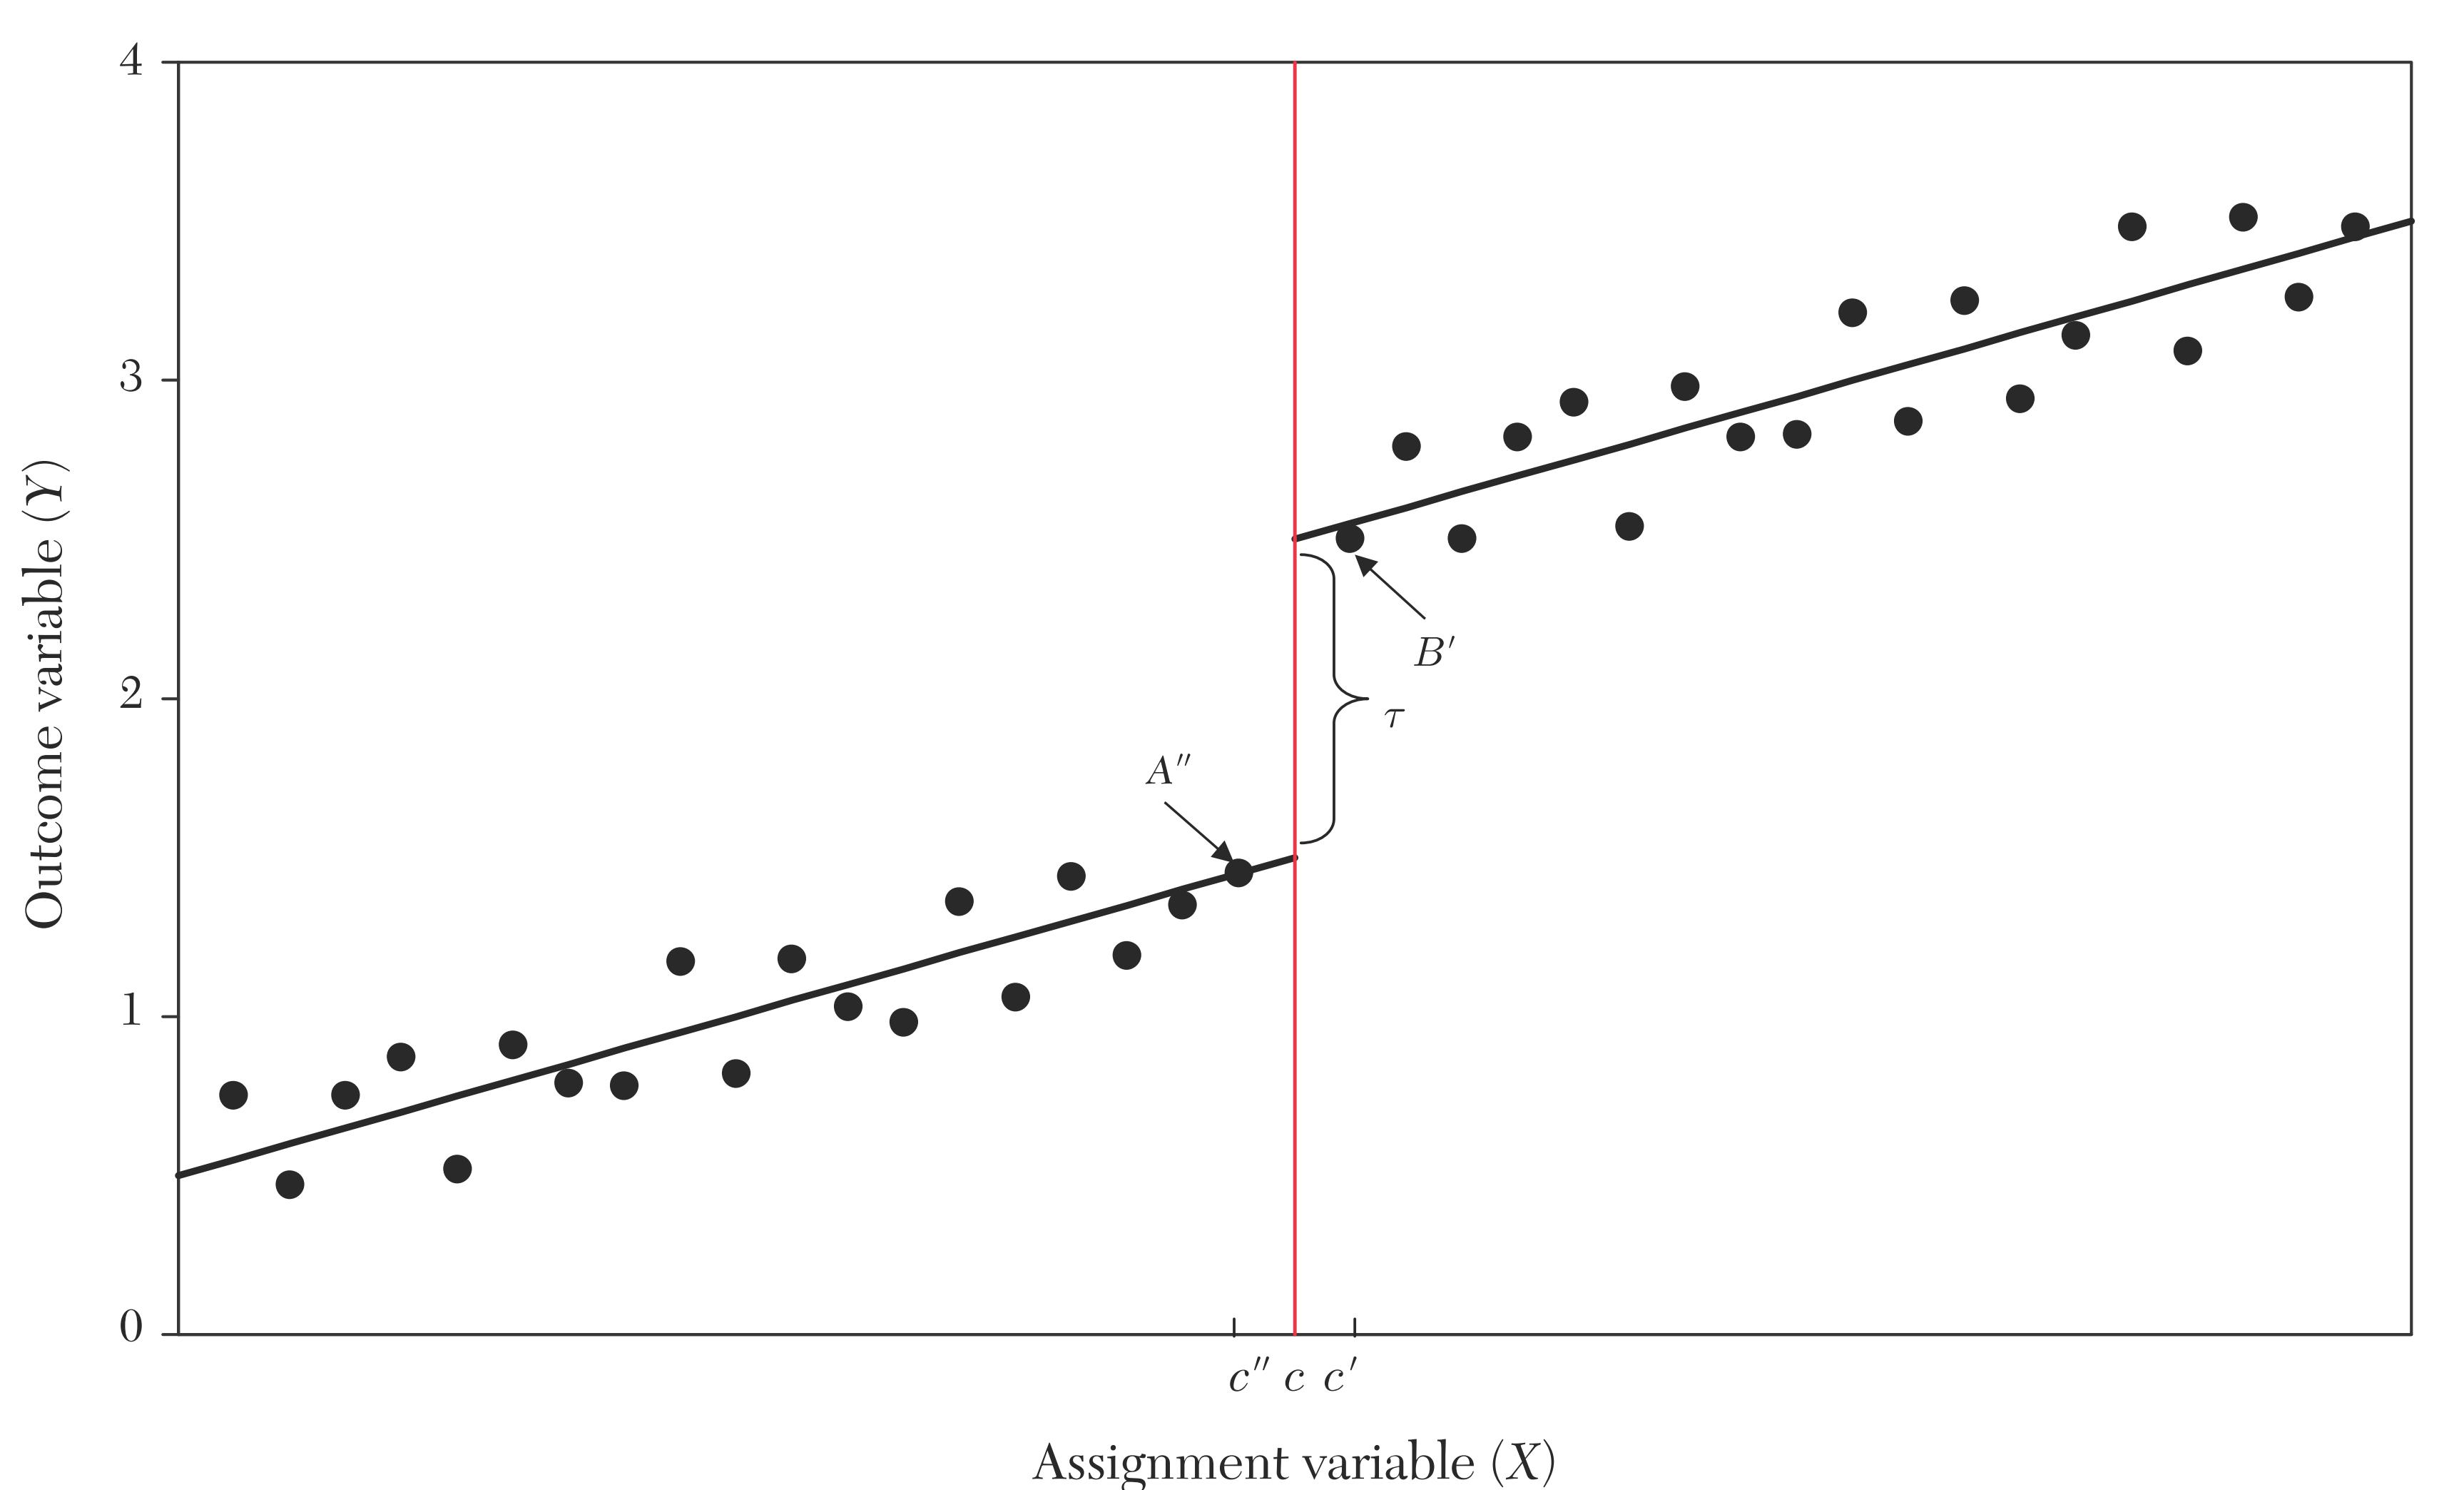
\includegraphics[width=1.0\textwidth]{figure/RD_score_f1.jpg}
	\end{figure}
	\begin{minipage}{0.9\linewidth}
		\fontsize{8}{8pt}\selectfont
		\emph{Source:} Lee and Lemieux (2010)
	\end{minipage}
\end{center}


\end{frame}







\begin{frame}{Main Idea of Regression Discontinuity Design}{A Motivating Example}

Mark Hoekstra (2009) ``\textbf{The Effect of Attending the Flagship State University on Earnings: A Discontinuity-Based Approach}" Review of Economics and Statistics

\begin{itemize}

%\item ``Where there is a cutoff there is a RD"
%\vspace{0.2cm}
%\item Fortunately, it is typical for selective schools and programs to use fairly strict grade cutoffs for admission
\item This paper demonstrates the above RD idea by examining the economic return of attending the most selective public state
university

\vspace{0.2cm}
\item In the United States, most schools used SAT (or ACT) scores in
their admission process
\vspace{0.2cm}
\item For example, the flagship state university considered here uses a strict cutoff based on SAT score and high school GPA

\end{itemize}
\end{frame}

\begin{frame}{Main Idea of Regression Discontinuity Design}{A Motivating Example}
\begin{itemize}

\item For the sake of simplicity, Hoekstra just focuses on the SAT score (adjusted depending on GPA)
\vspace{0.2cm}
\item The author is then able to match (using social security numbers) students applying to the flagship university in 1986-89 to their
administrative earnings data for 1998 to 2005
\vspace{0.2cm}
\item As in any good RD study, pictures tell it all, so let's just focus on
those

\end{itemize}
\end{frame}



\begin{frame}{SAT Score and Enrollment}

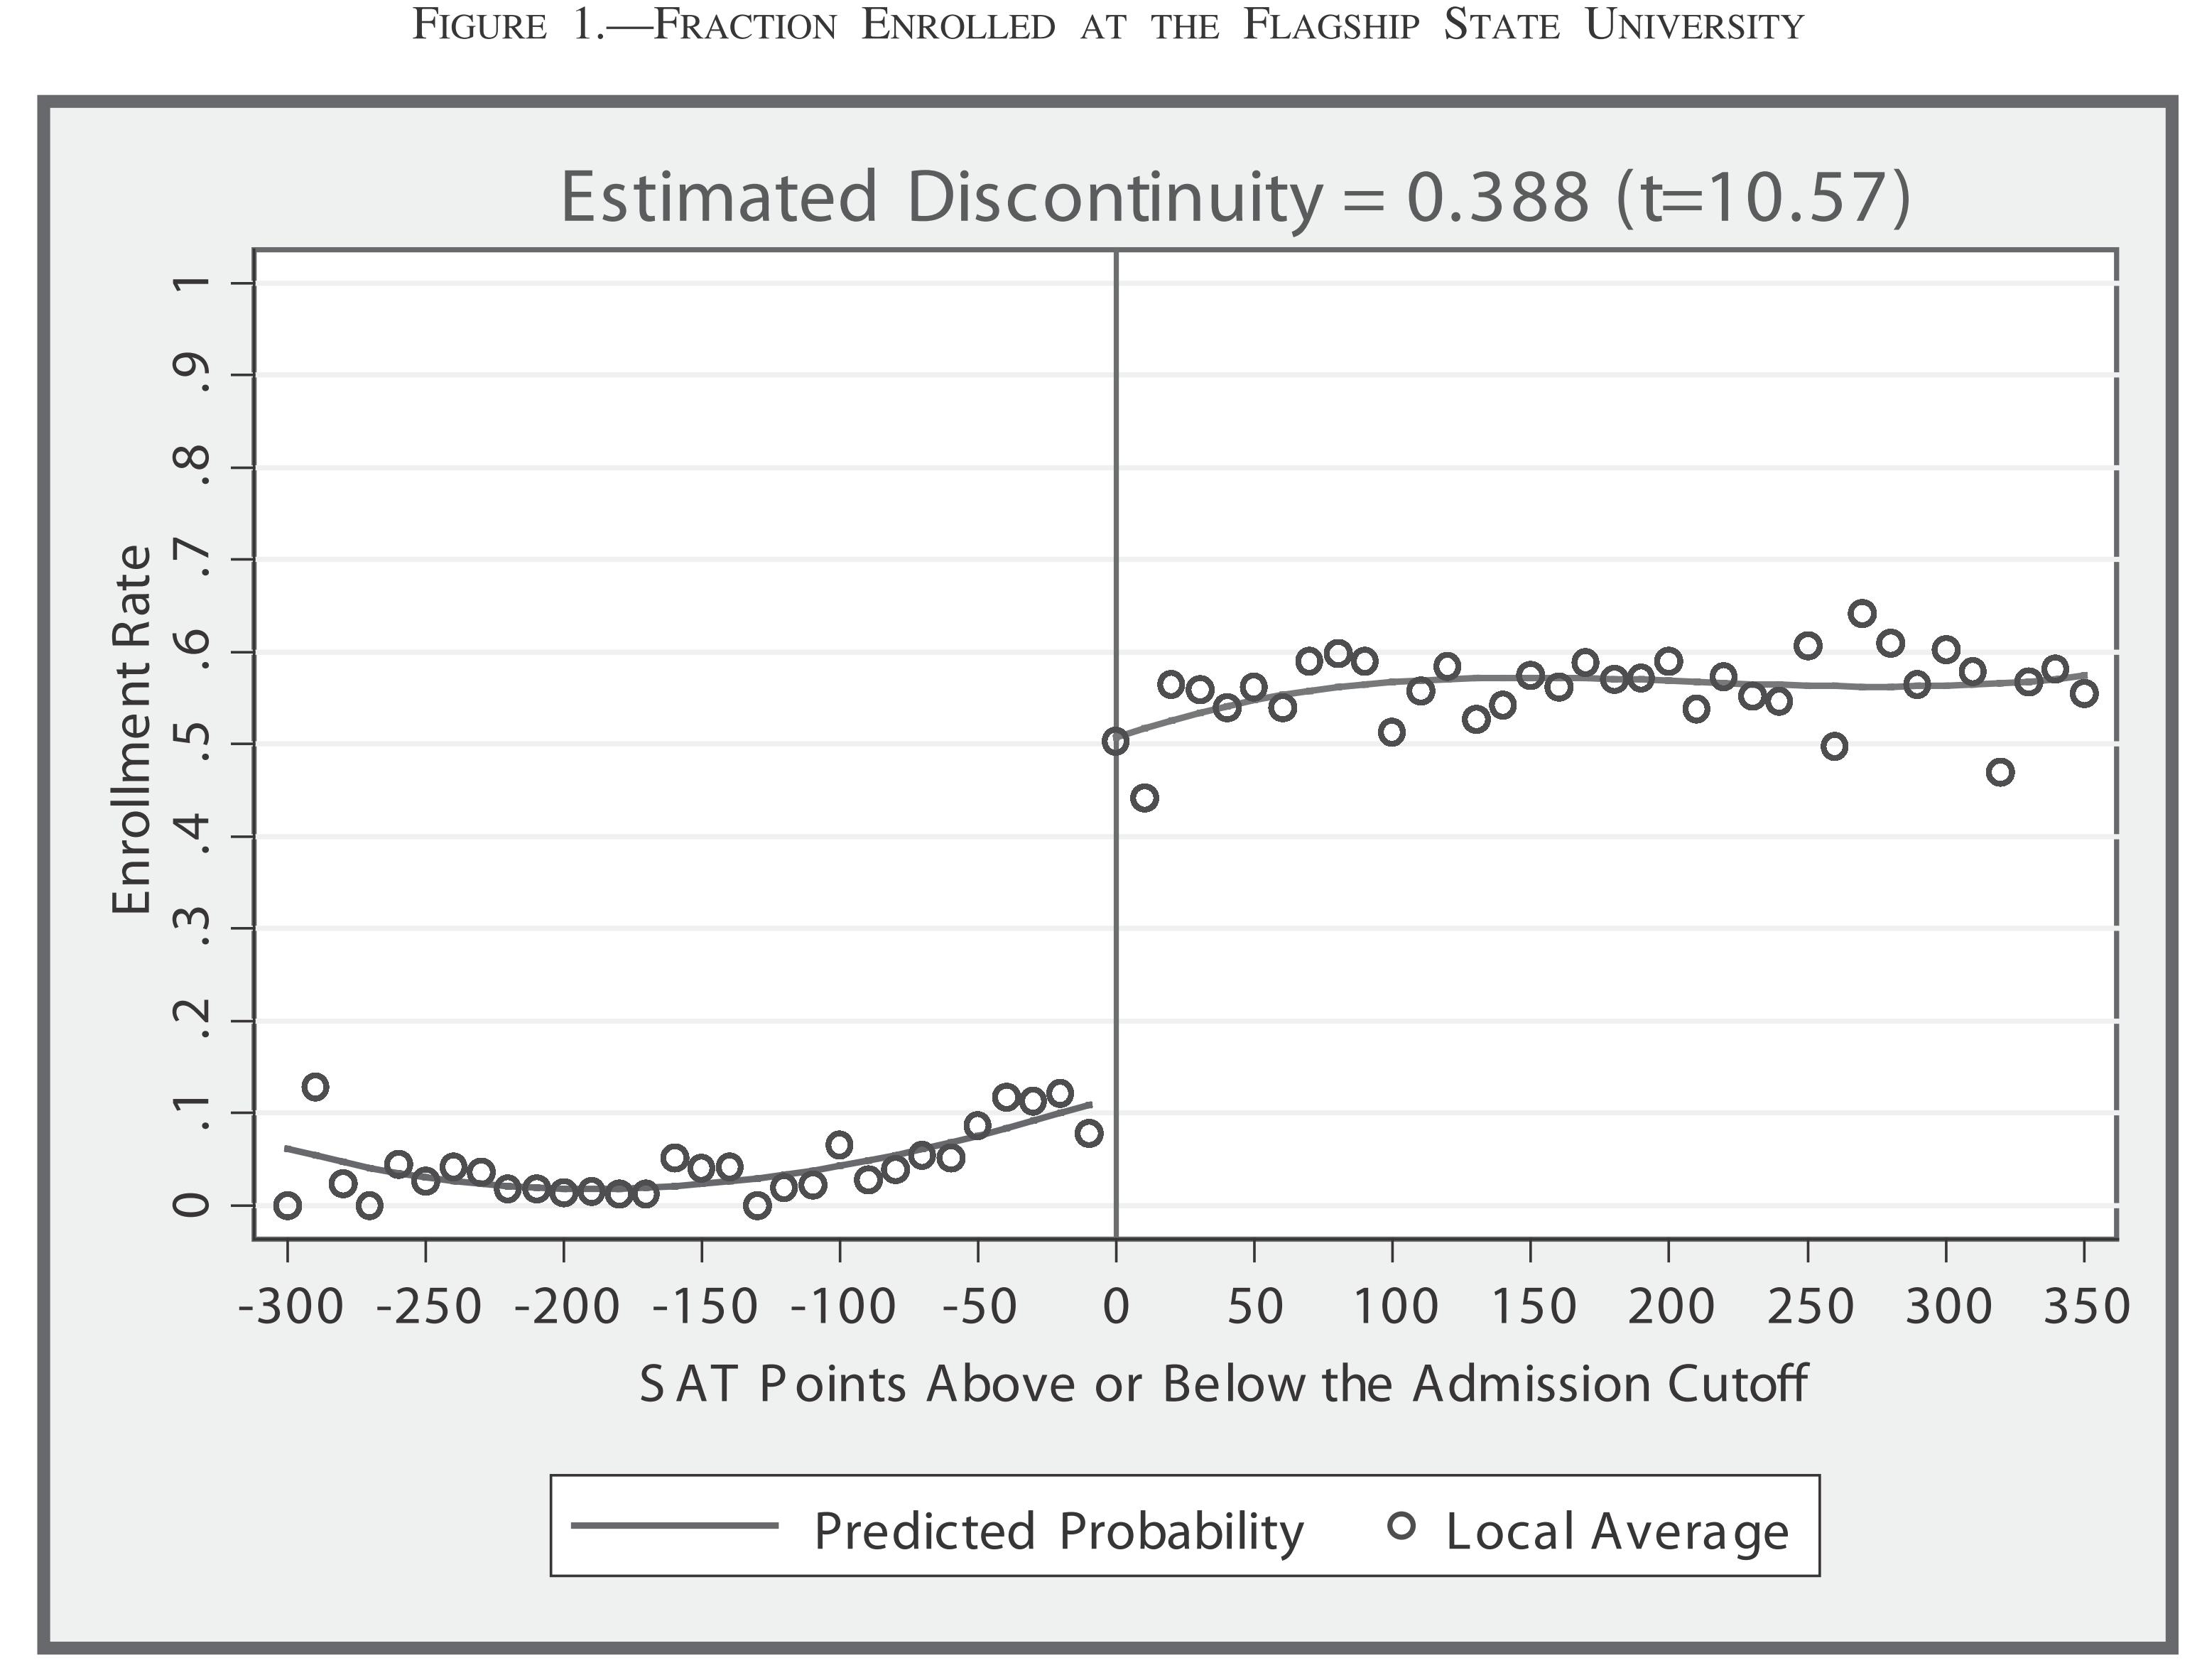
\includegraphics[width=1.0\textwidth]{figure/college_f1.jpg}


\end{frame}



\begin{frame}{SAT Score and Earnings}

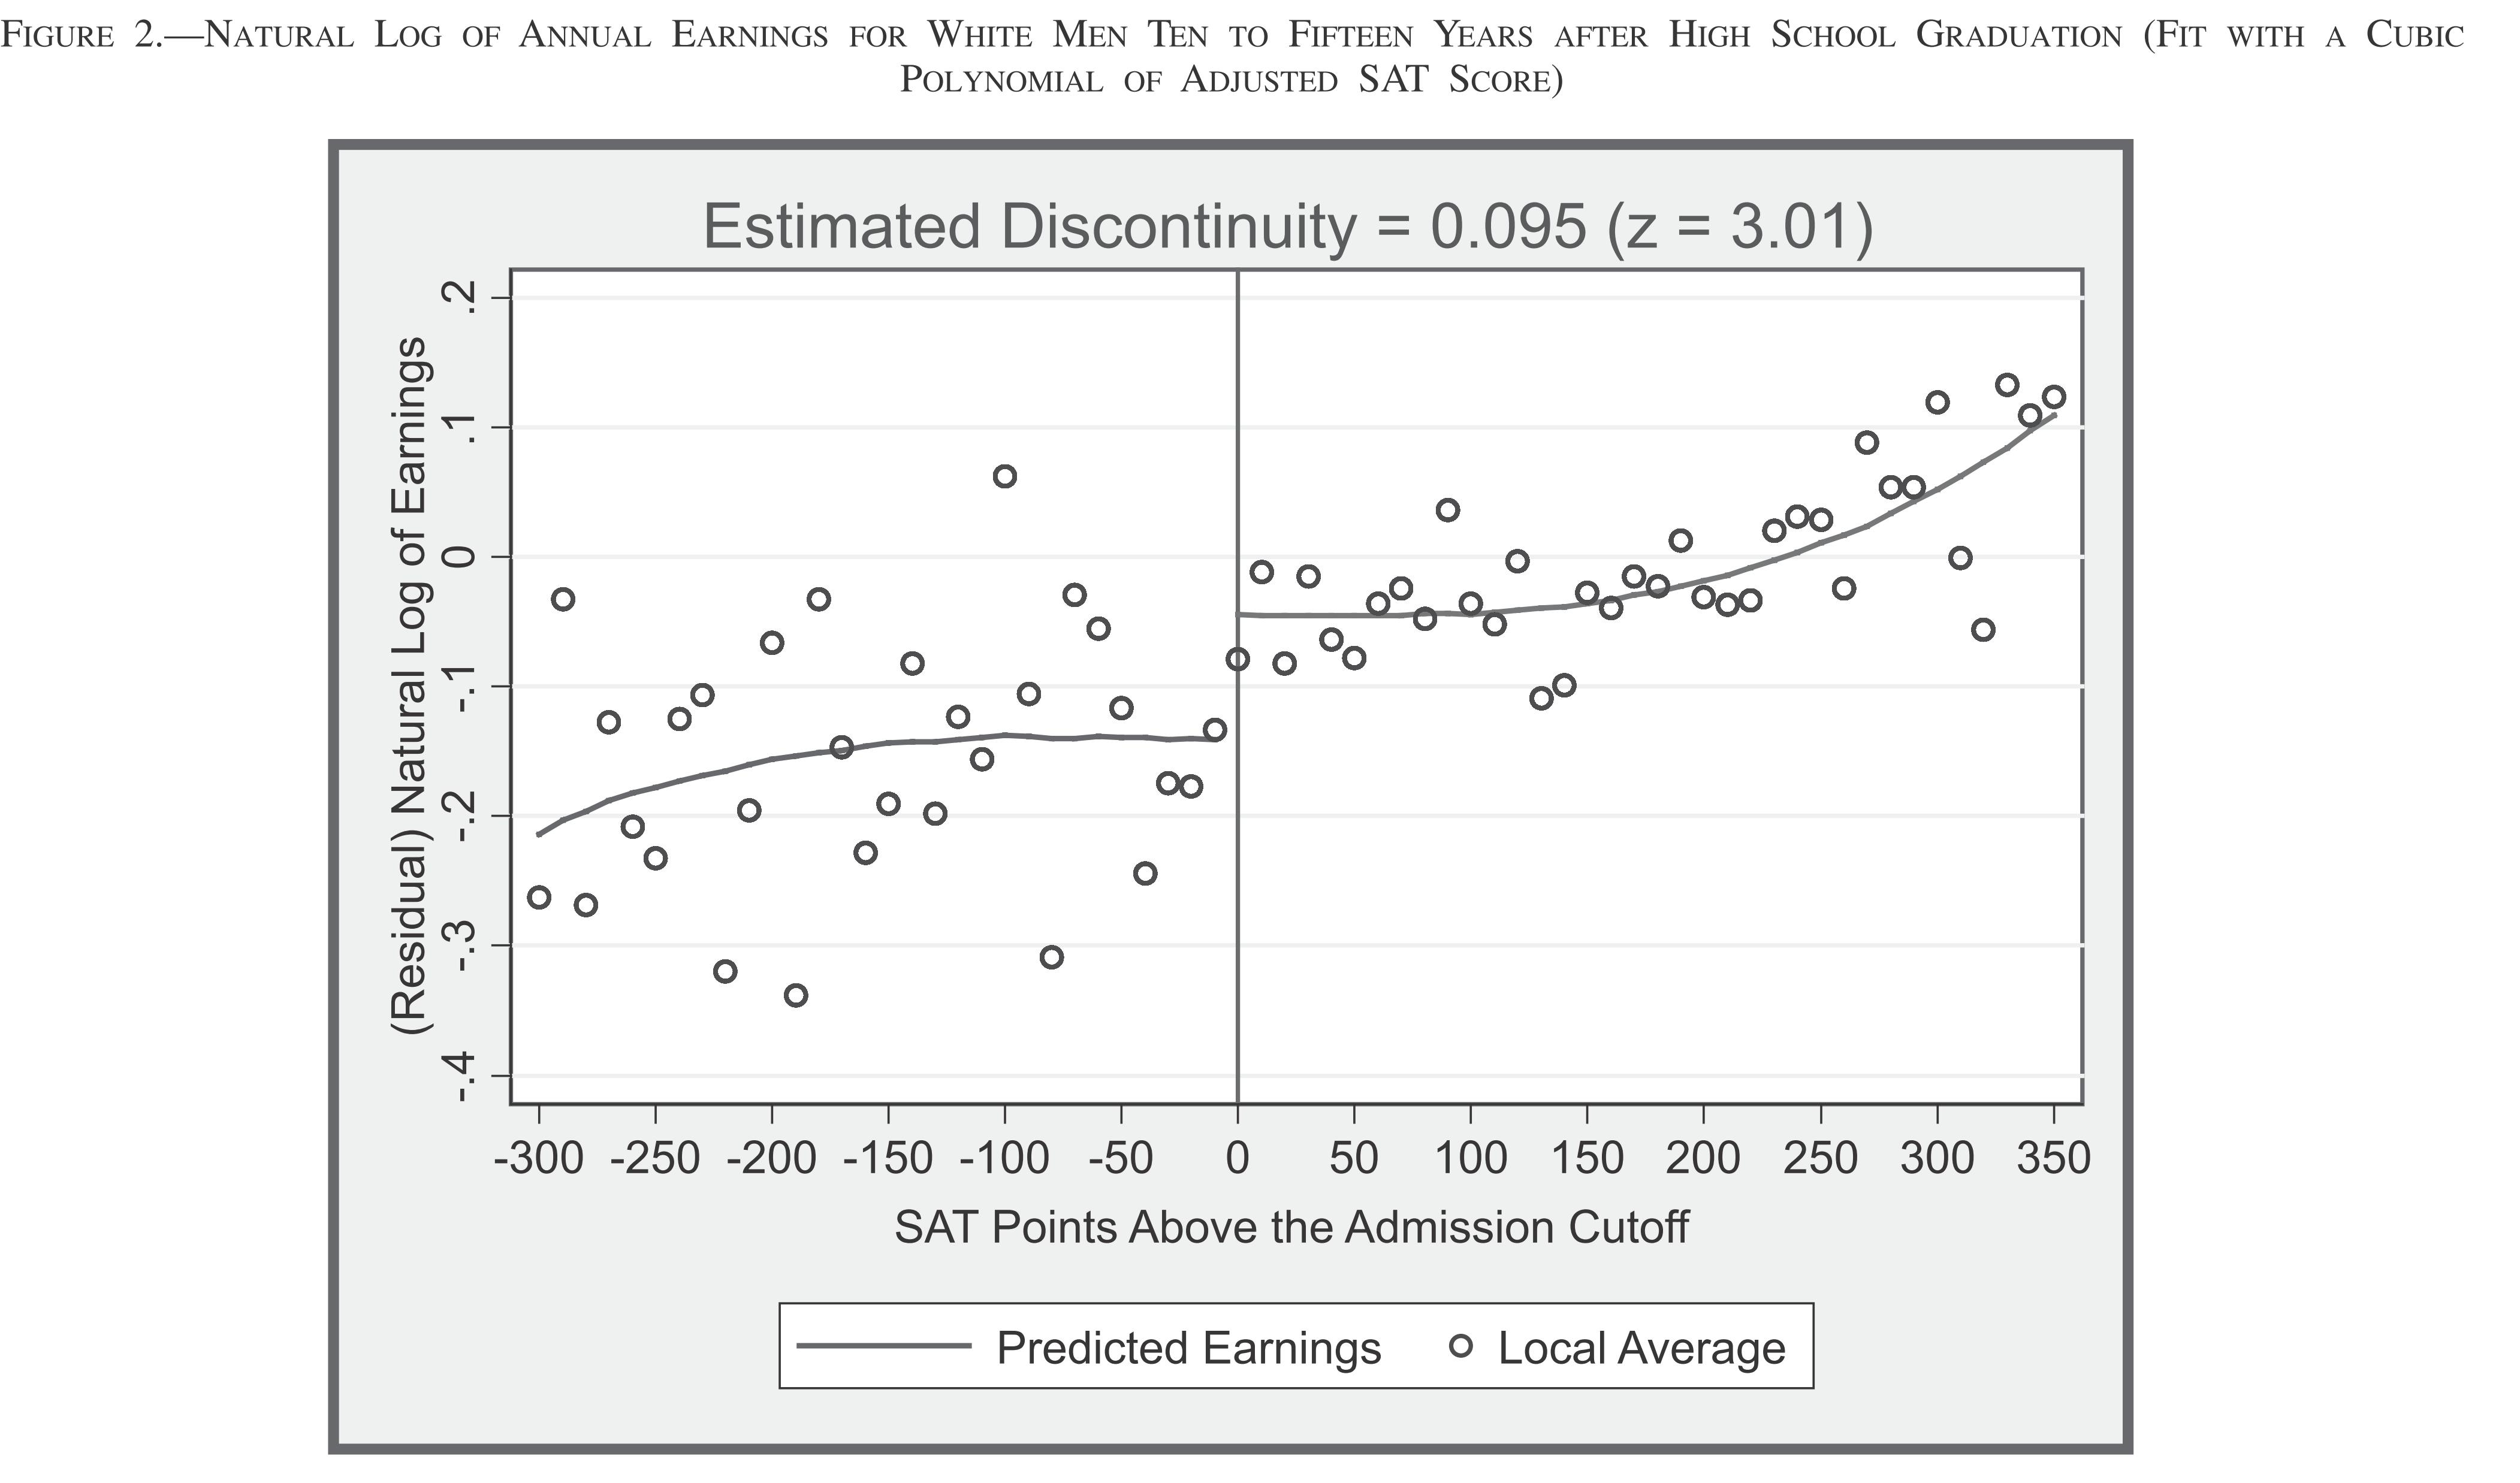
\includegraphics[width=1.0\textwidth]{figure/college_f2.jpg}


\end{frame}



\begin{frame}{More Examples}{}
\begin{itemize}

\item \textbf{Where there is a cutoff there is a RD}

\end{itemize}
\end{frame}




\begin{frame}{Public Health}{The Effect of Health Intervention}

Prashant Bharadwaj, Katrine Vellesen Løken, and
Christopher Neilson (2013) ``\textbf{Early Life Health Interventions and Academic Achievement}" AER

\begin{itemize}

\item The effect of \textbf{health intervention} in early childhood on \textbf{later life outcomes}
\vspace{0.2cm}
\item \textbf{Selection bias}: children who need health intervention in early childhood could be very sick and might have bad later life outcome (e.g. low educational attachment)

\end{itemize}
\end{frame}




\begin{frame}{Public Health}{The Effect of Health Intervention}
\begin{itemize}


\item \textbf{RDD solution}: 
\vspace{0.2cm}
\begin{itemize}
\item Infants with a birth weight below \textbf{1500 grams} were eligible for additional healthcare while those with a birth weight just above the cutoff were not eligible
\vspace{0.2cm}
\end{itemize}
\item Compares mortality rates and academic achievement between those infants \textbf{just below and above the cutoff of 1500 grams} 
\end{itemize}
\end{frame}




\begin{frame}{}

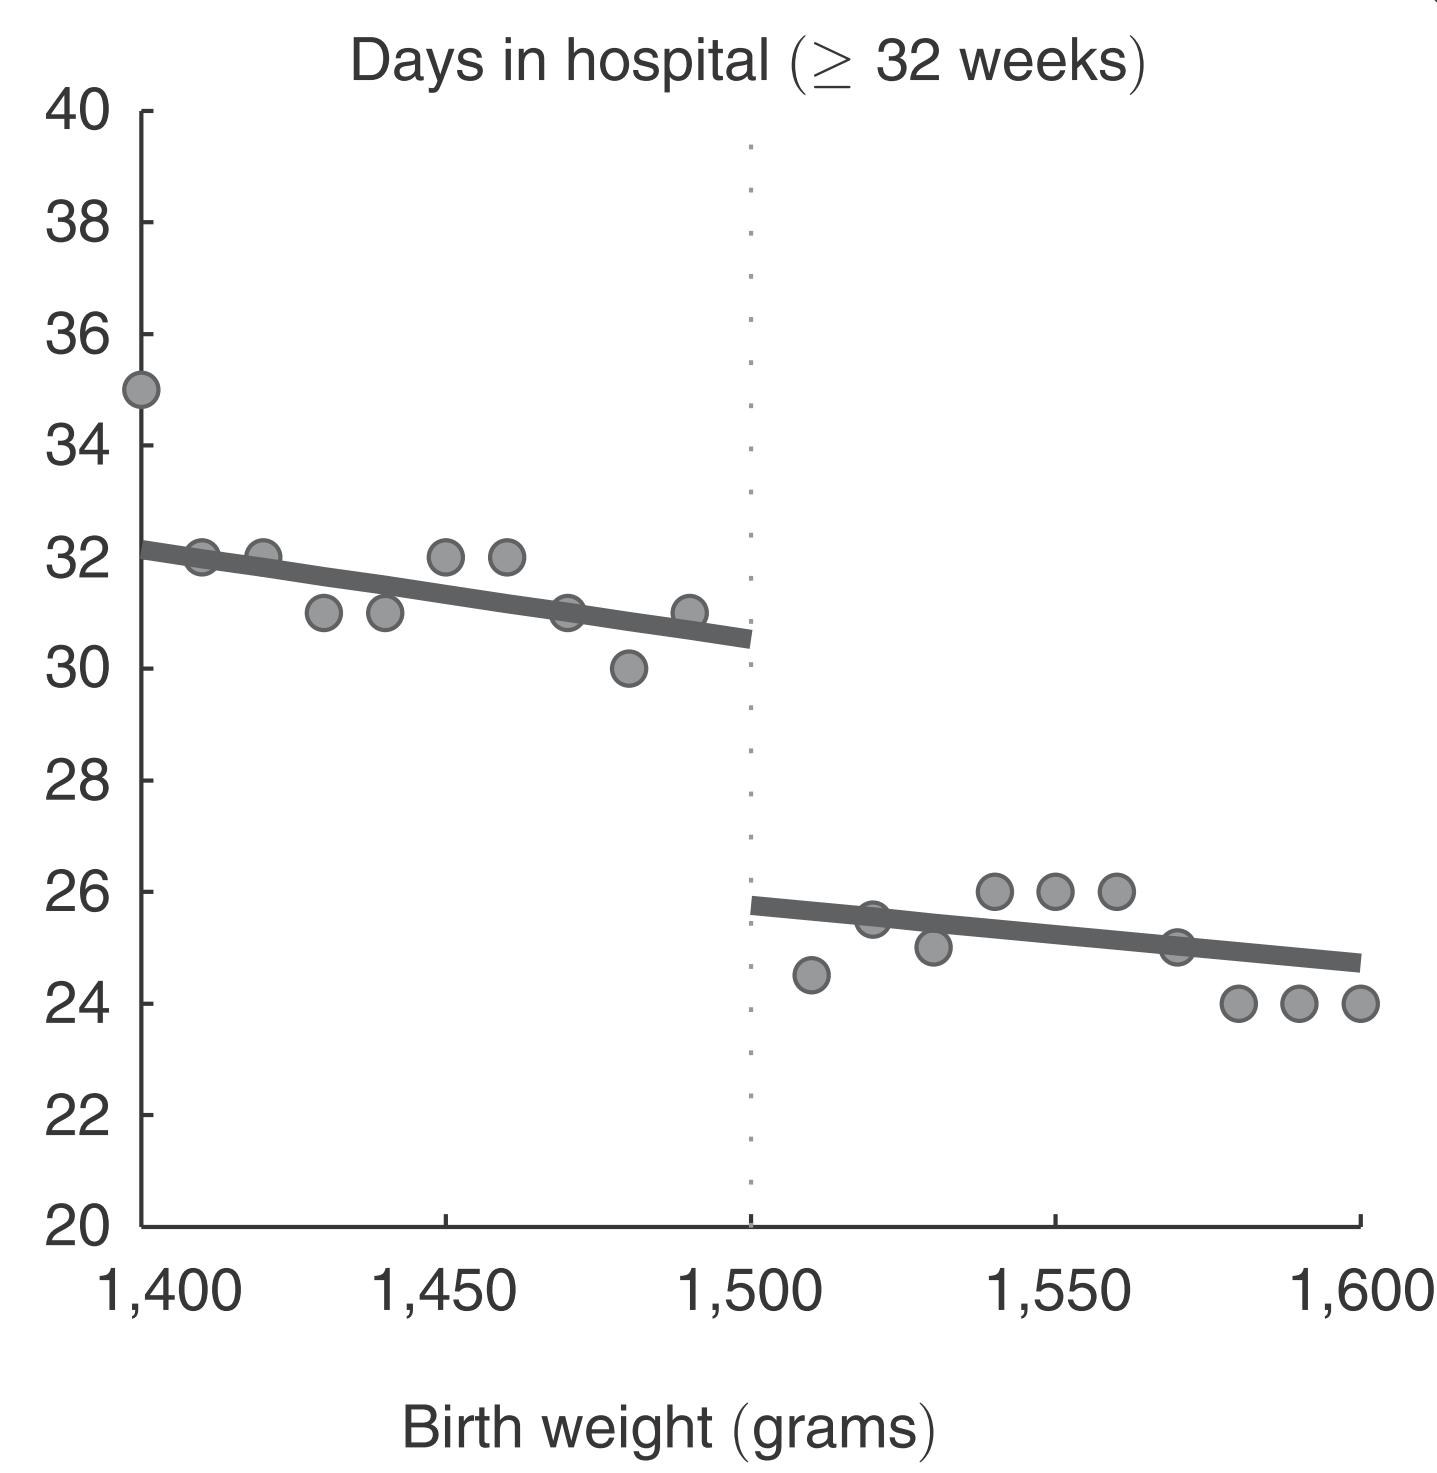
\includegraphics[width=0.7\textwidth]{figure/RD_health_f1.jpg}


\end{frame}


\begin{frame}{}

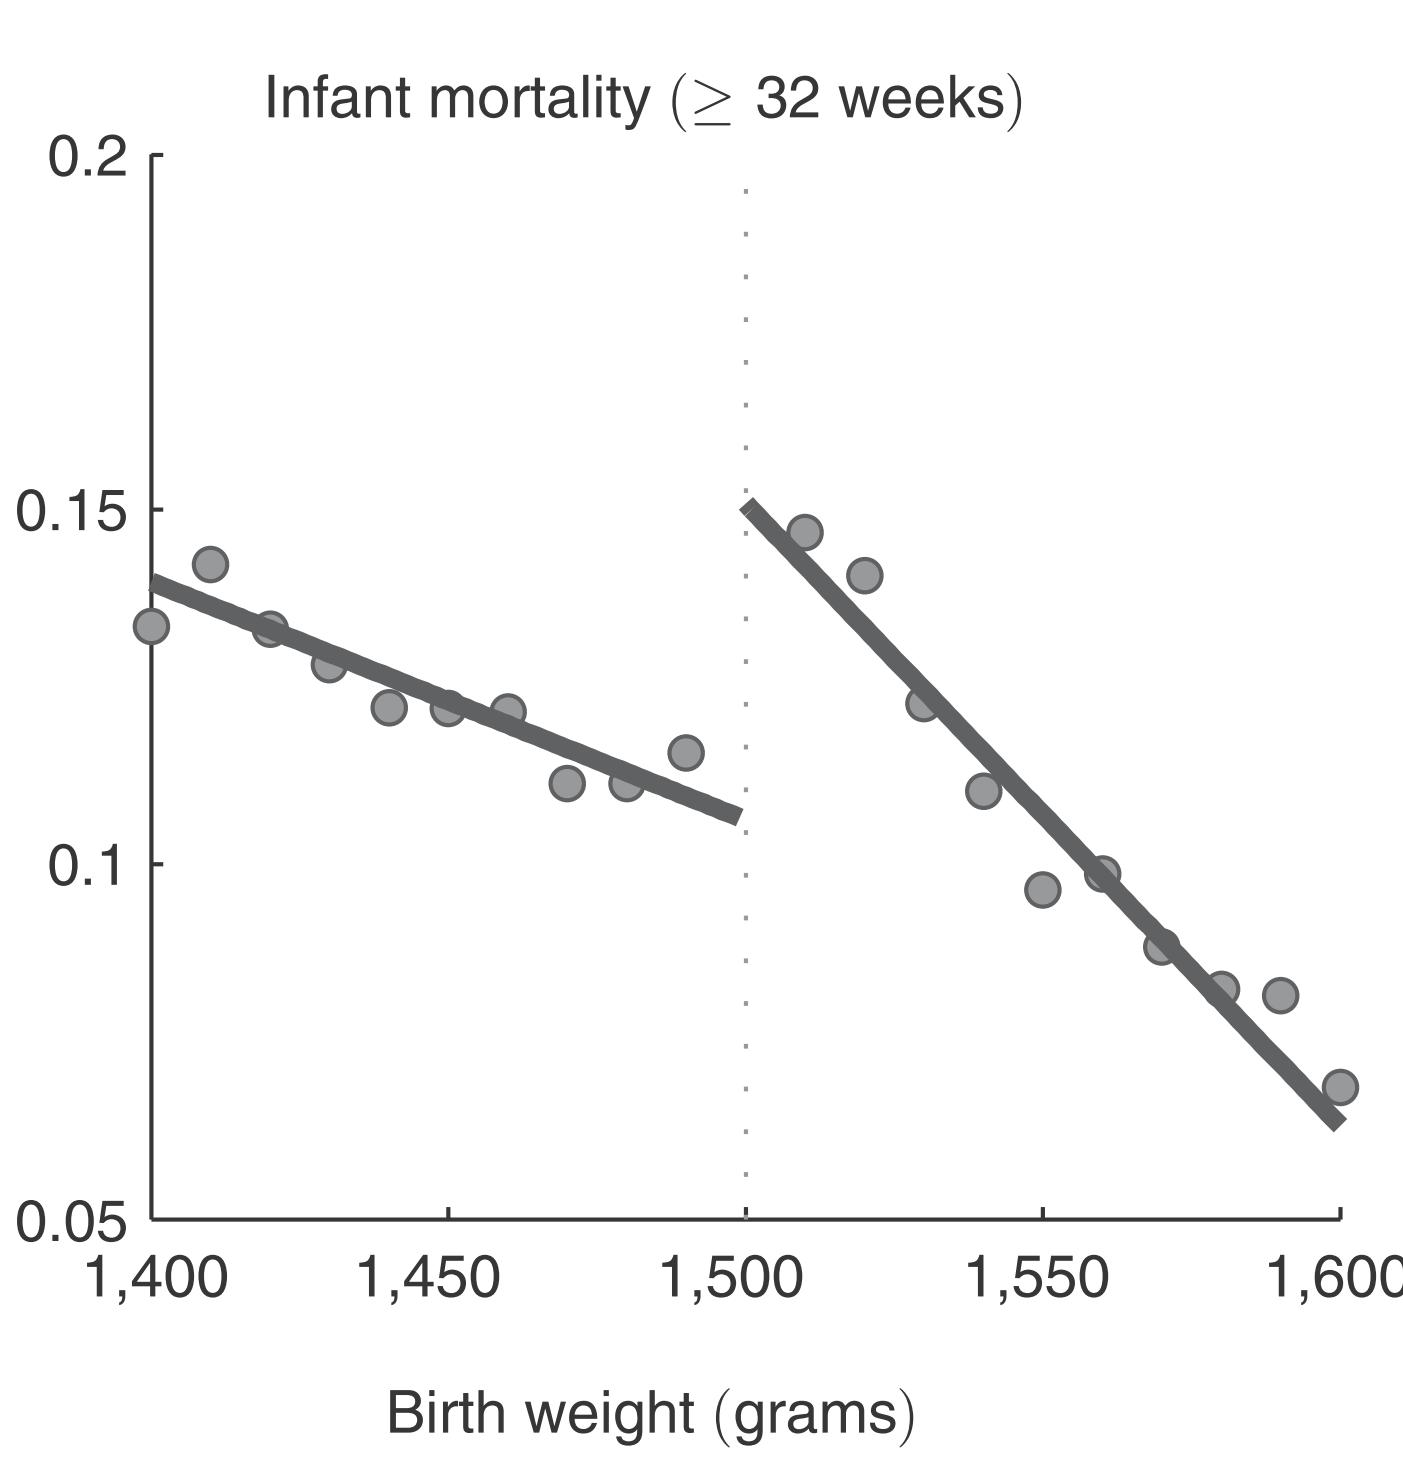
\includegraphics[width=0.7\textwidth]{figure/RD_health_f2.jpg}


\end{frame}


\begin{frame}{}

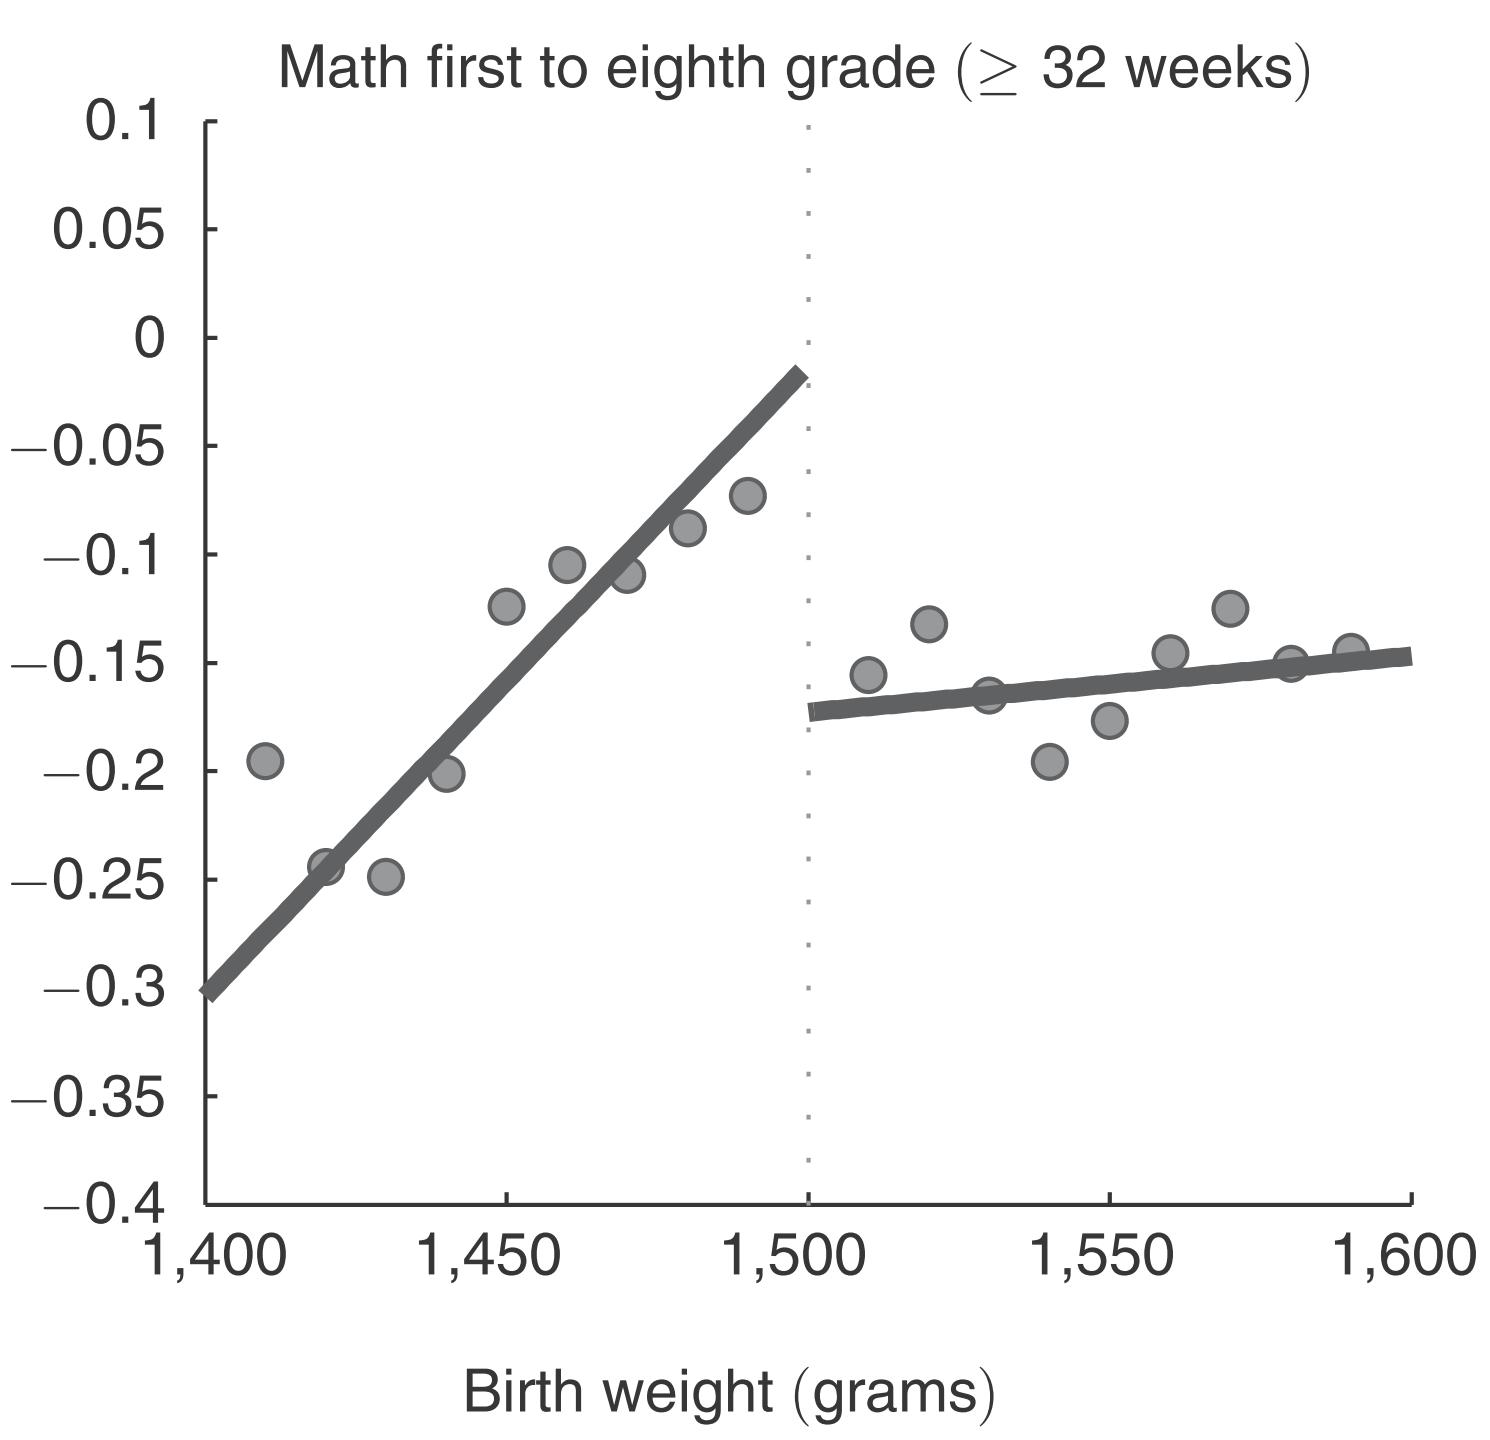
\includegraphics[width=0.7\textwidth]{figure/RD_health_f3.jpg}


\end{frame}


\begin{frame}{Political Science}{The Effect of Incumbency}

David Lee (2007) ``\textbf{Randomized Experiments from Non-random Selection in U.S. House Elections}" Journal of Econometrics

\begin{itemize}

\item  Does \textbf{political incumbency} provide an \textbf{electoral advantage}
\vspace{0.2cm}
\item \textbf{Selection bias}: people who win election (incumbency) should be more popular

\end{itemize}
\end{frame}




\begin{frame}{Political Science}{The Effect of Incumbency}
\begin{itemize}
	
	\item \textbf{RDD solution}: 
	\vspace{0.2cm}
	\begin{itemize}
		\item Candidates who just \textbf{barely won} an election (barely became the incumbent) are likely to be ex ante comparable in all other ways to candidates who \textbf{barely lost}
		\vspace{0.2cm}
		\item So their differential electoral outcomes in the \textbf{next election} should represent a true \textbf{incumbency advantage}
	\end{itemize}
\end{itemize}
\end{frame}



\begin{frame}{}

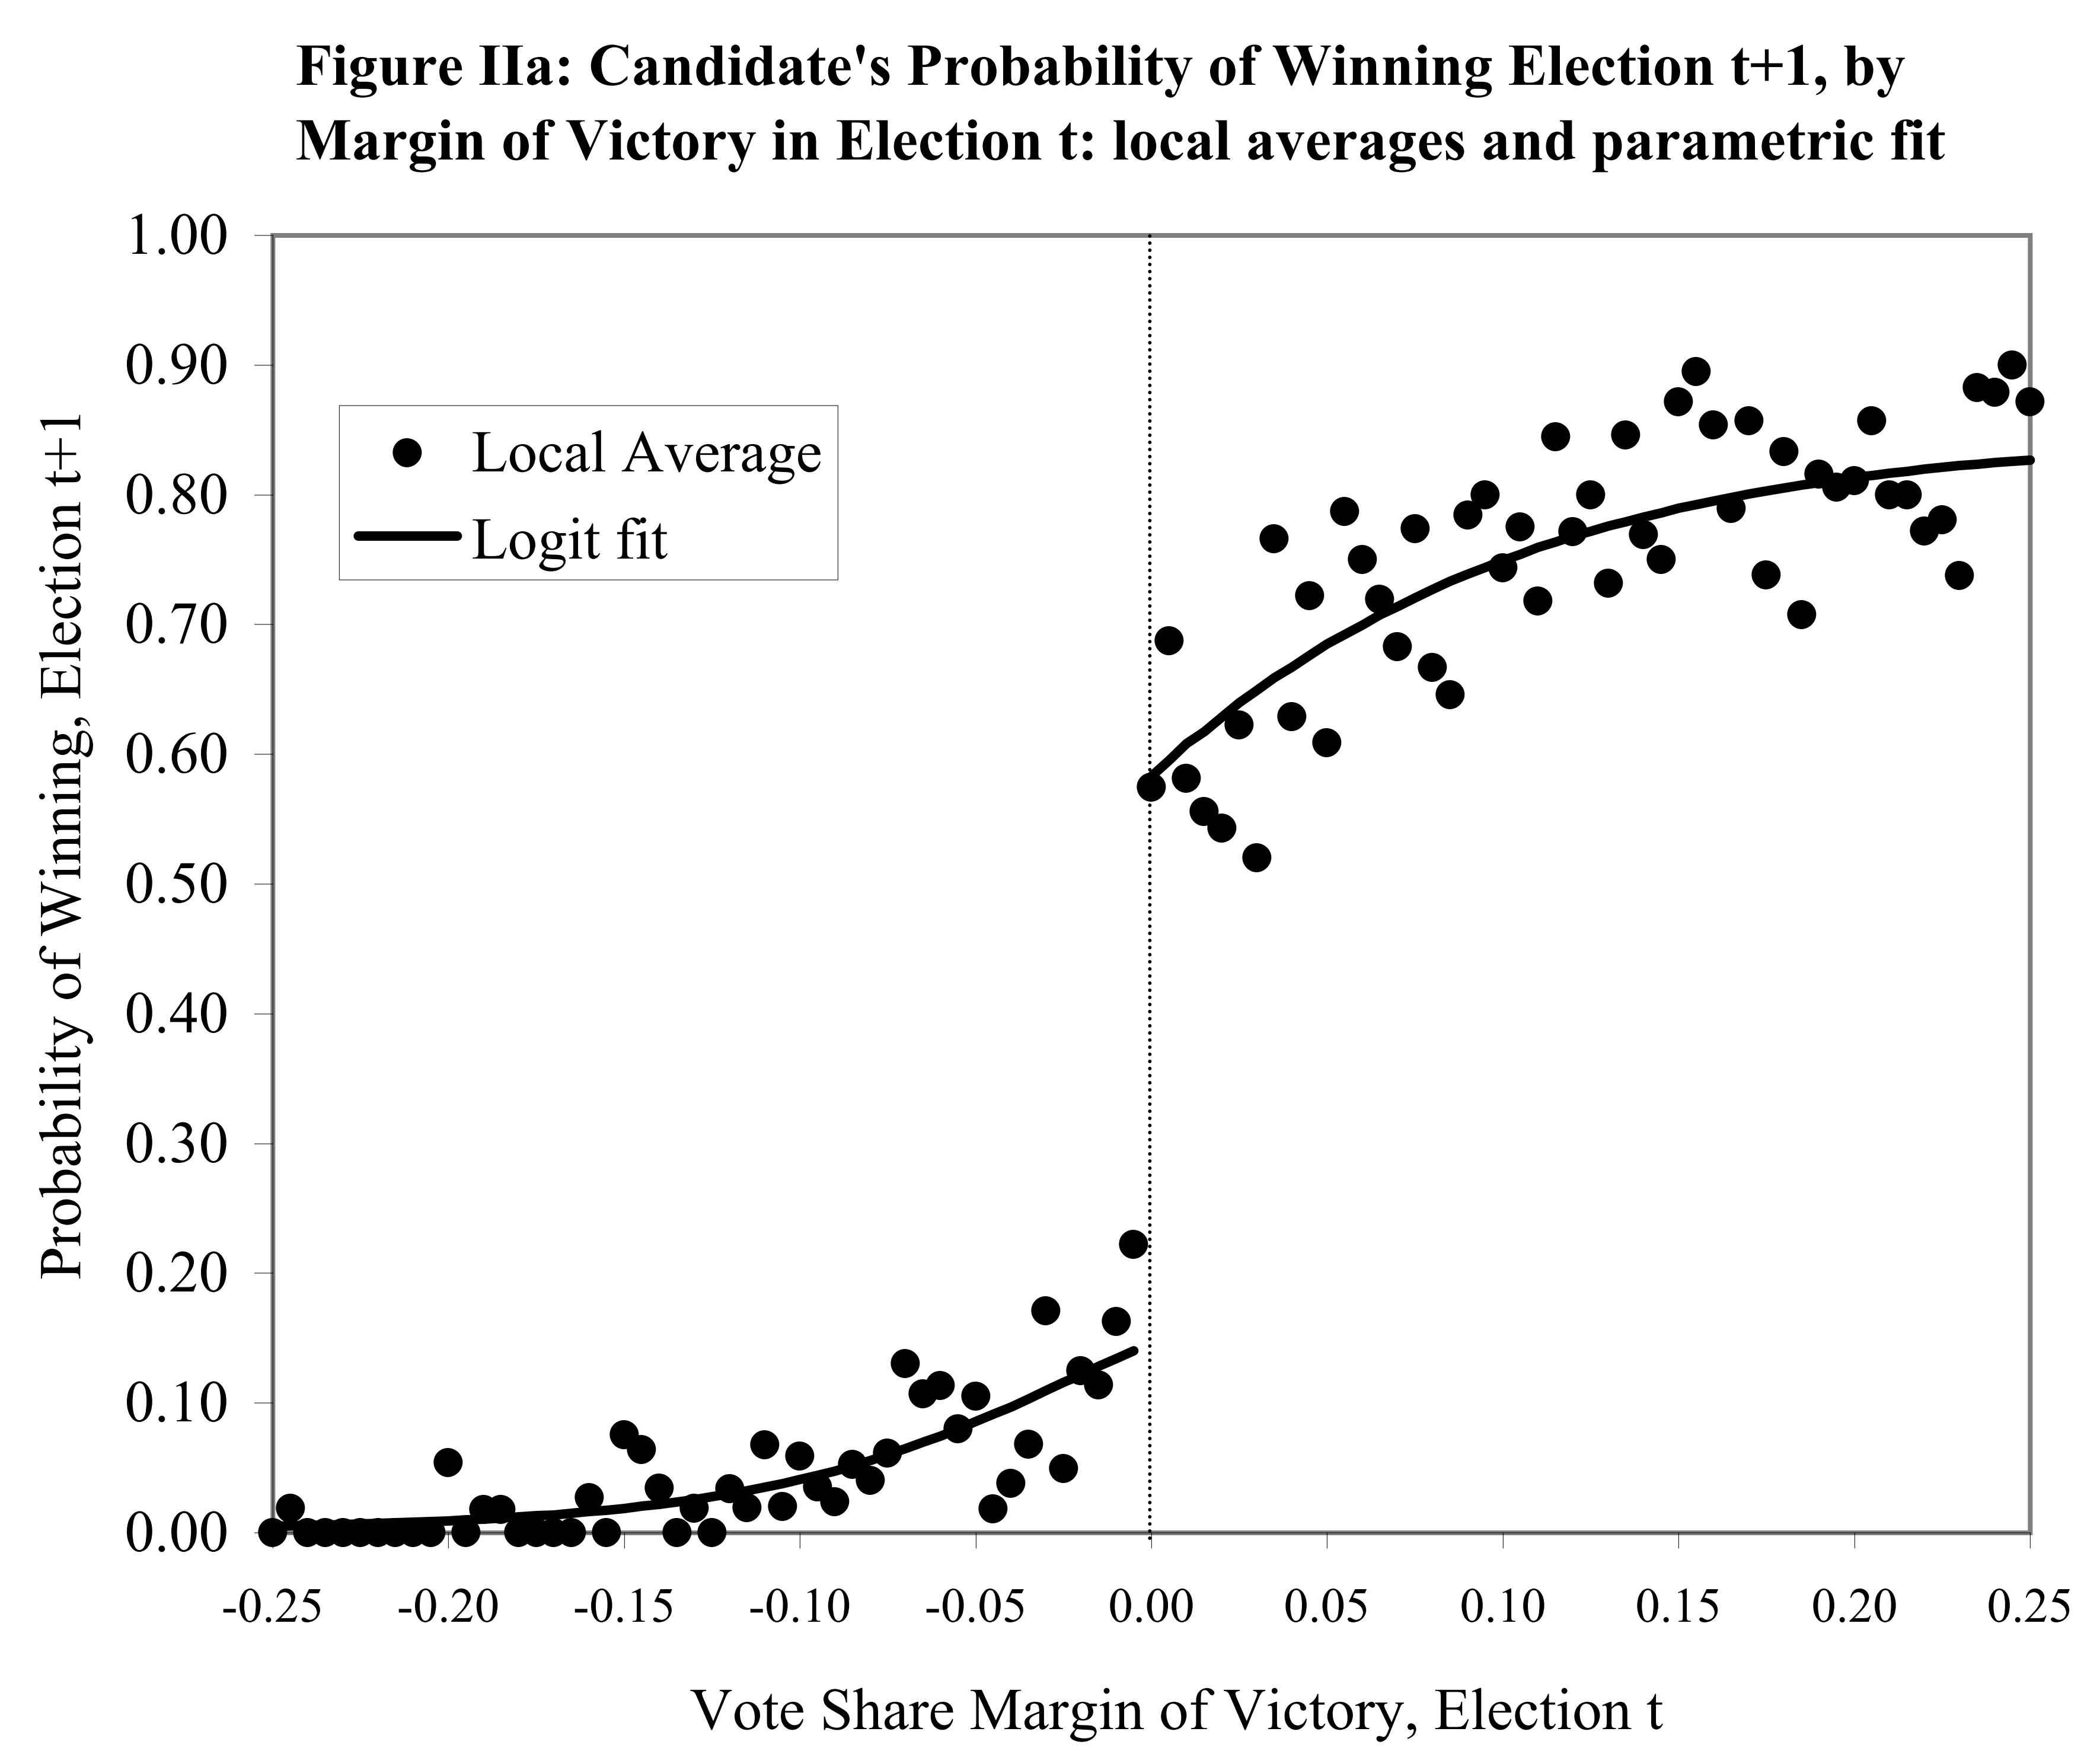
\includegraphics[width=0.9\textwidth]{figure/RD_poli_f1.jpg}


\end{frame}



\begin{frame}{Labor Economics}{Spatial Regression Discontinuity}
	Rafael Lalive (2008), ``\textbf{How do extended benefits affect unemployment duration?
		A regression discontinuity approach}", Journal of Econometrics
	\begin{itemize}
		\vspace{0.2cm}
		\item This paper studies a targeted program that extends the maximum duration of unemployment benefits from 30 weeks to 209 weeks in Austria
		\vspace{0.2cm}
		\item Sharp discontinuities in treatment assignment at age 50 and at the border between eligible regions and control regions identify the effect of \textbf{extended benefits} on \textbf{unemployment duration}
	\end{itemize}
\end{frame}


\begin{frame}{Labor Economics}{Spatial Regression Discontinuity}
	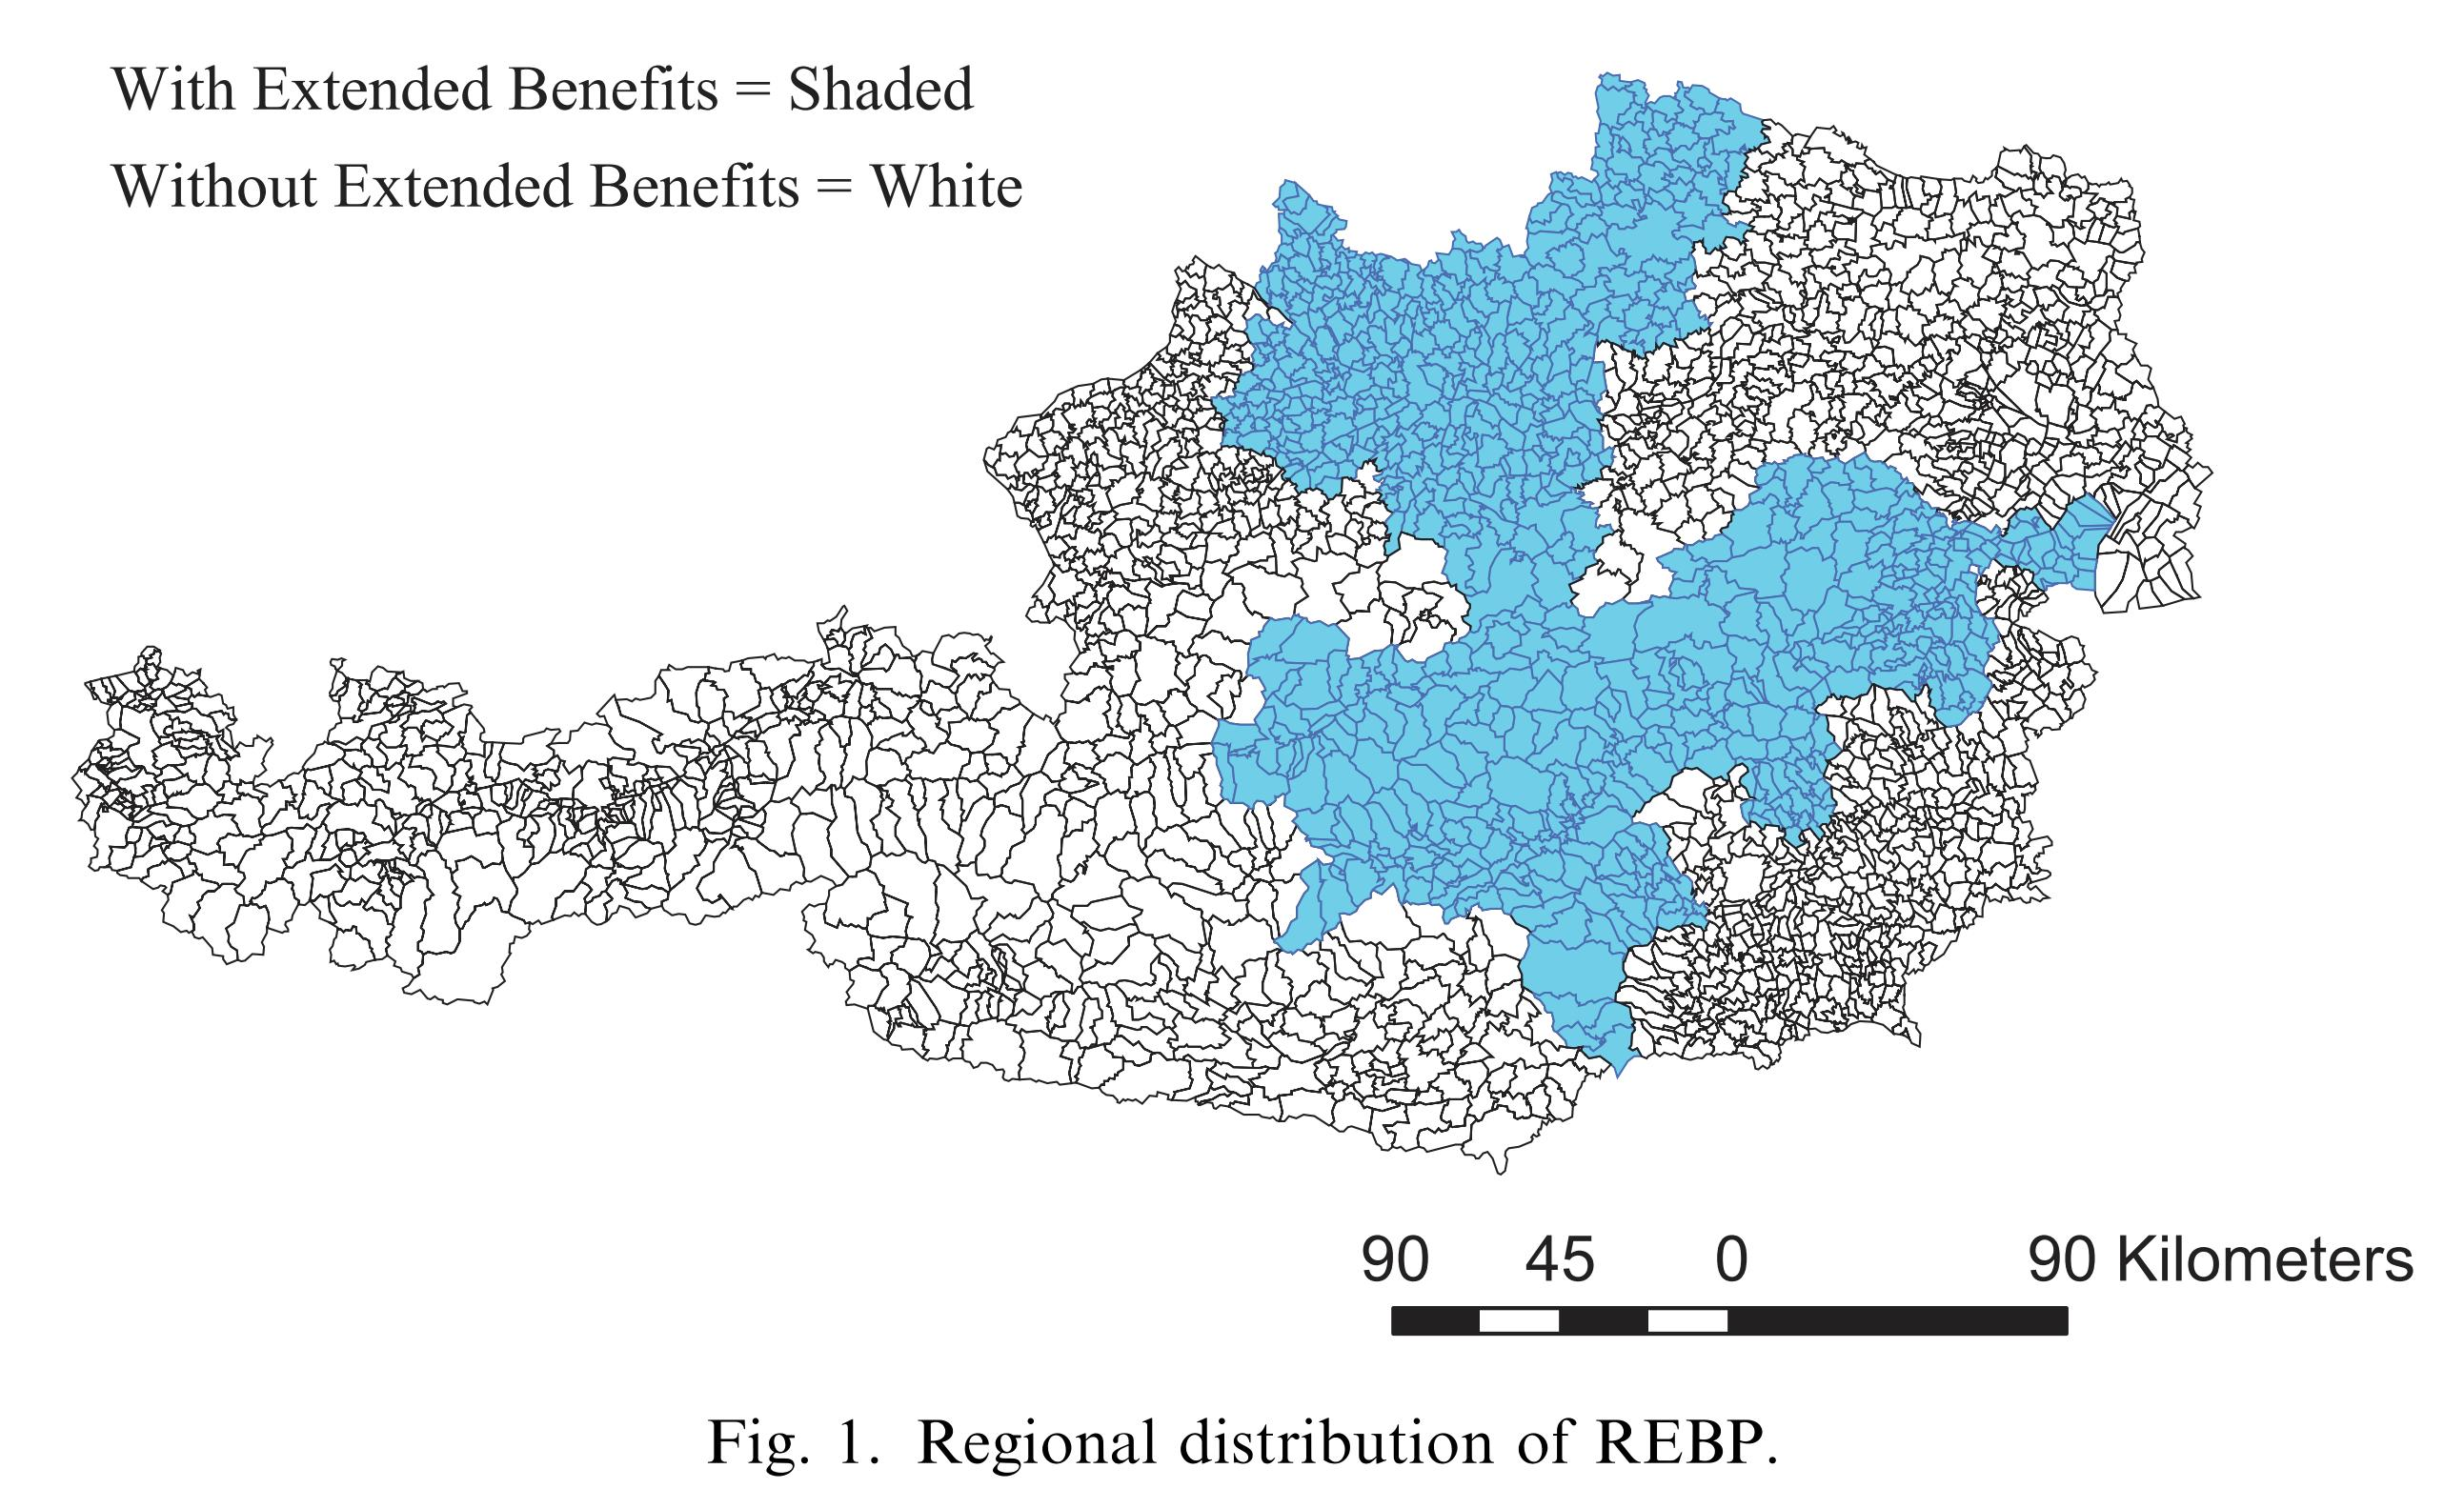
\includegraphics[width=.90\textwidth]{figure/srd_ui_f1.jpg}
	
\end{frame}


\begin{frame}{Labor Economics}{Spatial Regression Discontinuity}
	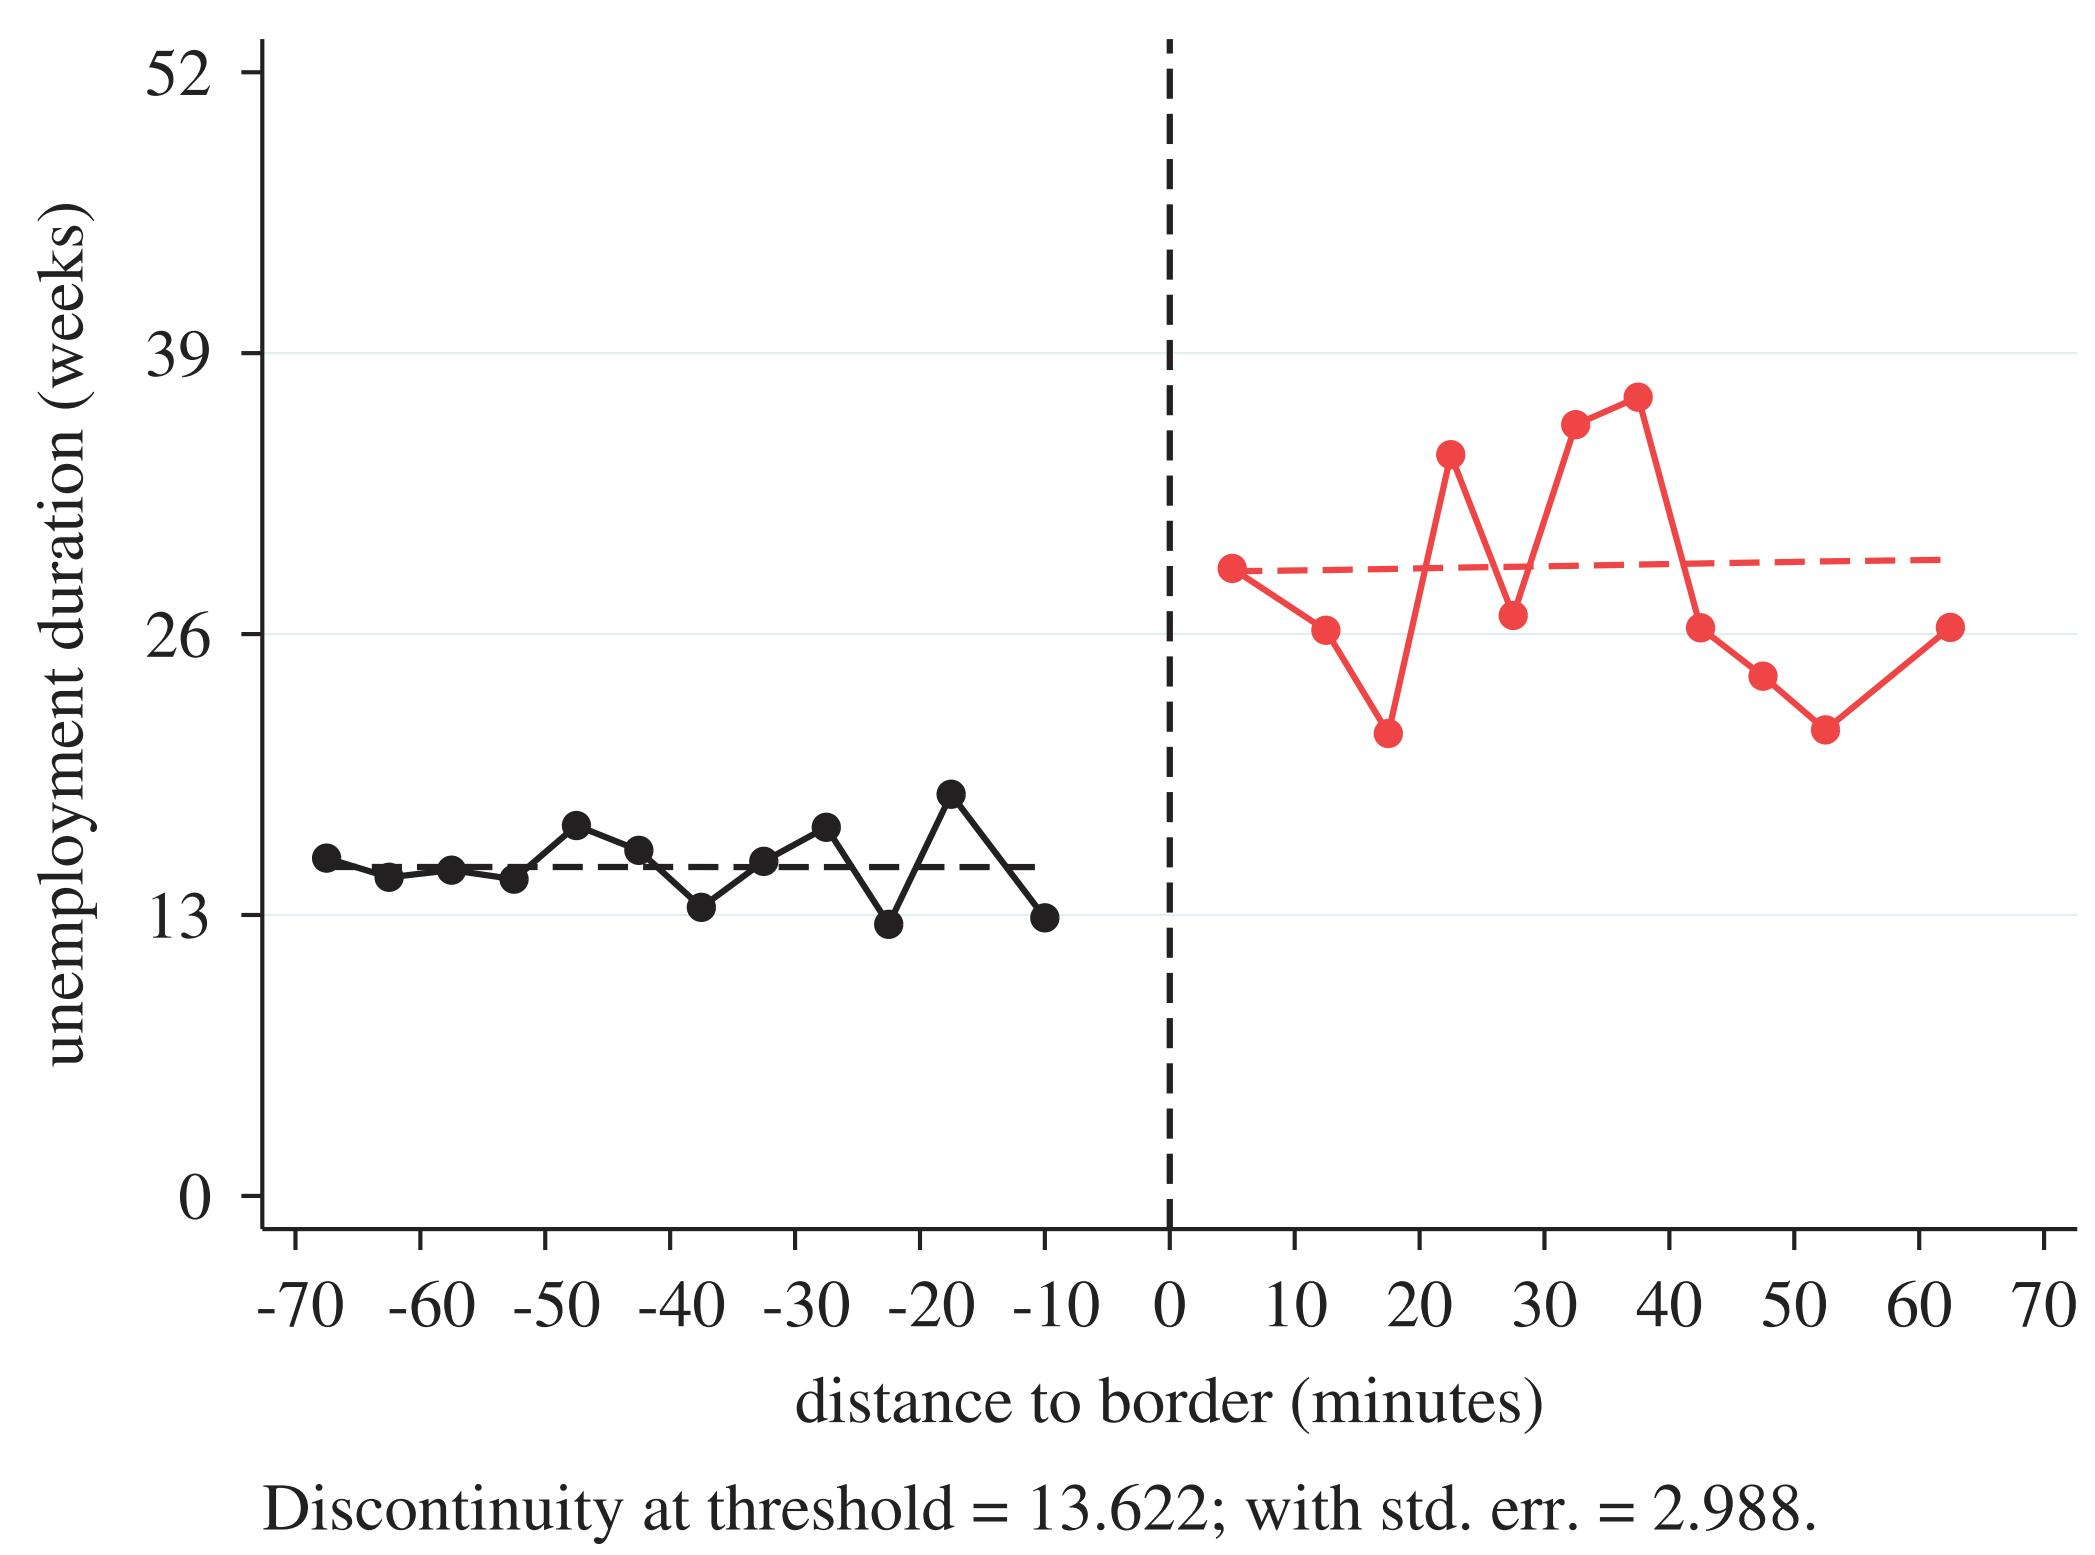
\includegraphics[width=.90\textwidth]{figure/srd_ui_f3.jpg}
	
\end{frame}



\begin{frame}{RDD Became Popular since late 1990s }{}
	
	\begin{itemize}
		\item The first RDD paper is Thistlethwaite and Campbell (1960), ``RD Analysis: An Alternative to Ex Post Fact
		Experiments," Journal of Education Psychology
		\vspace{0.2cm}
		\item RDD was not used much in economics until the late 1990s
		\vspace{0.2cm}
		\item But hundreds of studies since then, starting with Van der Klaauw (2002)
		\vspace{0.2cm}
		\item Two possible explanations:
		\vspace{0.2cm}
		\begin{itemize}
			\item Cutoff rules are very wide spread…
			\vspace{0.2cm}
			\item Much more data available now, especially administrative data sets
		\end{itemize}
		
	\end{itemize}
\end{frame}


\begin{frame}{RDD Became Popular since late 1990s }{}
	
	\begin{itemize}
		\item An important advantage of RD designs is that they are well suited to
		large administrative data sets with
		\vspace{0.2cm}
		\begin{itemize}
			\item Few covariates
			\vspace{0.2cm}
			\item Lots of observations and all the relevant information about cutoffs and assignment variables 
			\vspace{0.2cm}
			\item Since those have to be used in the administration of programs
		\end{itemize}
		
		
	\end{itemize}
\end{frame}



\begin{frame}{Sharp RDD and Fuzzy RDD}{}
	
	\begin{itemize} 
		
		\item In general, depending on enforcement of treatment assignment, RDD can be categorized into two types:
		
				\begin{itemize} 	
		\vspace{0.2cm}
		
				\item[1] {\color{blue}Fuzzy RDD}: the probability of getting the treatment jumps discontinuously at the cutoff 
		\vspace{0.2cm}
		
		\item[2] {\color{blue}Sharp RDD}: the probability of getting the treatment jumps from 0 to 1 at the cutoff 

%		\vspace{0.2cm}
%		\begin{itemize}
%			\item Everyone follows treatment assignment rule (all are compliers) 	
%			\vspace{0.2cm}	 
%			\item Local randomized experiment with perfect compliance around cutoff
%			
%			
%		\end{itemize}
		\vspace{0.2cm}
		

%		\begin{itemize}
%			\item Not everyone follows treatment assignment rule  	
%			\vspace{0.2cm}	 
%			\item Local randomized experiment with partial compliance around cutoff
%			\vspace{0.2cm}	 
%			\item  Using initial assignment as an instrument (IV) for actual treatment
%			
%		\end{itemize}
		
			\end{itemize}
		
	\end{itemize}
\end{frame}



%
%
%\begin{frame}{Fuzzy RDD}{Overview}
%	\begin{itemize}
%		
%		%\item So far, we focus on sharp RDD
%		
%		
%		\item {\color{blue}Fuzzy RDD}: 
%		
%		\begin{itemize}
%			\vspace{0.2cm}
%			\item The probability of getting the treatment is no longer a deterministic function of the assignment variable $A_{i}$
%			\vspace{0.2cm}
%			\item But there is still a discontinuity in the probability of getting treatment at the threshold
%		\end{itemize}
%		
%		
%	\end{itemize}
%\end{frame}









\begin{frame}{Fuzzy RDD}{Overview}
	\begin{itemize}
		
		\begin{block}{Fuzzy RDD}
			\begin{equation*}
				\lim_{\varepsilon\rightarrow 0}\Pr[D_i=1|A_i=c+\varepsilon] - \lim_{\varepsilon\rightarrow 0}\Pr[D_i=1|A_i=c-\varepsilon] \neq 0
			\end{equation*}
		\end{block}
		
	
			\vspace{0.2cm}
			\item The probability of getting the treatment jumps discontinuously at the cutoff 
			\vspace{0.2cm}
			\begin{itemize}
				\item Some individuals above cutoff do NOT get treatment and some individuals below cutoff do receive treatment
			\end{itemize}
		\end{itemize}
		
		
		%\begin{itemize}		
		%	\item The probability of being admitted to elite university may jump at a certain test score 
		% \vspace{0.2cm}
		%	\item Students still can decide not enroll in that school
		%\end{itemize}
		

\end{frame}









\begin{frame}{Treatment Probability and assignment variable}{Fuzzy RDD}
	\begin{figure}
		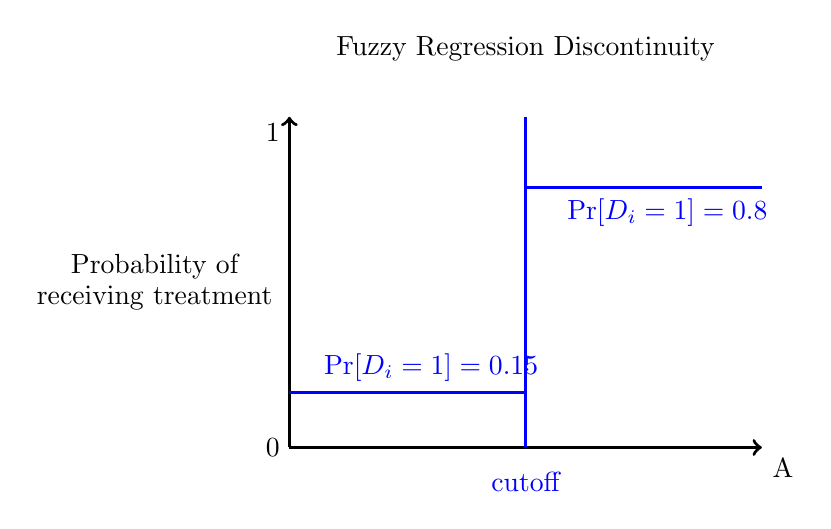
\begin{tikzpicture}[comment/.style={rectangle, text centered}]
			\centering
			\draw[very thick,->] (0,0) -- (6,0) node[anchor=north west] {A};
			\draw[very thick,->] (0,0) -- (0,4.2) node[anchor=south east] {};
			
			\draw[very thick, blue] (3,4.2) -- (3,0) node[anchor=south, yshift=-0.7cm](3_0) {cutoff};
			\draw[very thick, blue] (0,0.7) -- (3,0.7)   node[anchor=south, xshift=-1.2cm] {$\Pr[D_i=1]=0.15$};
			\draw[very thick, blue] (3,3.3) -- (6,3.3)   node[anchor=north, xshift=-1.2cm] {$\Pr[D_i=1]=0.8$};
			
			\draw (0,0) -- (0,0) node[anchor=east](0_0) {$0$};
			\draw (0,4) -- (0,4) node[anchor=east] {$1$};
			
			\node [comment, above of = 3_0, yshift=4.5cm] {Fuzzy Regression Discontinuity};
			\node [comment, left of  = 0_0, yshift=2.3cm, xshift=-0.5cm] {Probability of};
			\node [comment, left of  = 0_0, yshift=1.9cm, xshift=-0.5cm] {receiving treatment};
		\end{tikzpicture}
	\end{figure}
\end{frame}







\begin{frame}{Sharp RDD}{Overview}
	\begin{itemize}
		
		\begin{block}{Sharp RDD}
		\begin{equation*}
			\lim_{\varepsilon\rightarrow 0}\Pr[D_i=1|A_i=c+\varepsilon] - \lim_{\varepsilon\rightarrow 0}\Pr[D_i=1|A_i=c-\varepsilon] = 1
		\end{equation*}
	\end{block}

			\item Sharp RDD is a special case of fuzzy RDD
			\vspace{0.2cm}		
			\item It further required the jump in probability to be from 0 to 1
			\vspace{0.2cm}
			\begin{itemize}
				\item Nobody below the cutoff gets the ``treatment", everybody above the cutoff gets it
			\end{itemize}

		
		
		
	\end{itemize}
\end{frame}



\begin{frame}{Treatment Probability and assignment variable}{Sharp RDD}
	\begin{figure}
		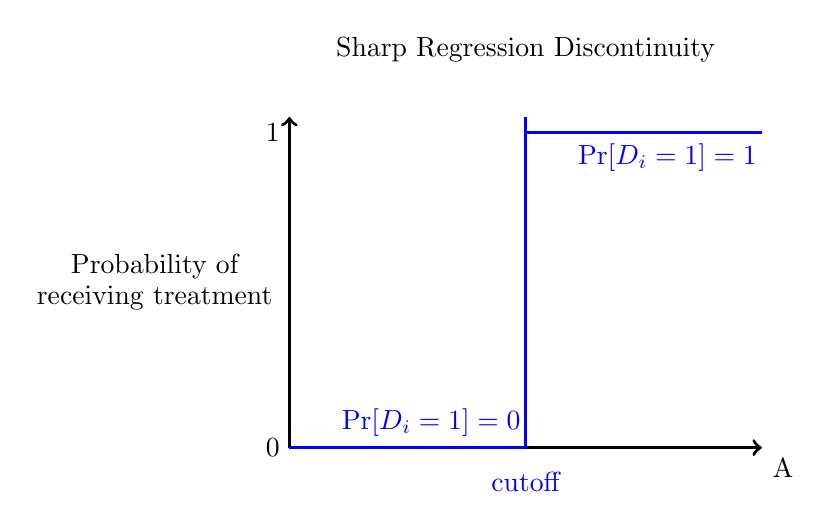
\begin{tikzpicture}[comment/.style={rectangle, text centered}]
			\centering
			\draw[very thick,->] (0,0) -- (6,0) node[anchor=north west] {A};
			\draw[very thick,->] (0,0) -- (0,4.2) node[anchor=south east] {};
			
			\draw[very thick, blue] (3,4.2) -- (3,0) node[anchor=south, yshift=-0.7cm](3_0) {cutoff};
			\draw[very thick, blue] (0,0) -- (3,0)   node[anchor=south, xshift=-1.2cm] {$\Pr[D_i=1]=0$};
			\draw[very thick, blue] (3,4) -- (6,4)   node[anchor=north, xshift=-1.2cm] {$\Pr[D_i=1]=1$};
			
			\draw (0,0) -- (0,0) node[anchor=east](0_0) {$0$};
			\draw (0,4) -- (0,4) node[anchor=east] {$1$};
			
			\node [comment, above of = 3_0, yshift=4.5cm] {Sharp Regression Discontinuity};
			\node [comment, left of  = 0_0, yshift=2.3cm, xshift=-0.5cm] {Probability of};
			\node [comment, left of  = 0_0, yshift=1.9cm, xshift=-0.5cm] {receiving treatment};
		\end{tikzpicture}
	\end{figure}
\end{frame}











\title[]  
{Identification}


\author 
{}

%\institute{Institute of Economics, Academia Sinica  \\ Econ, NTU}
%\institute{Institute of Economics, Academia Sinica  \\ IMES/IDAS, NTU}
\institute{}

%\author 
%{楊子霆 \\ 中研院經濟所}

%\institute 
%{中正大學國際經濟專題研討}




\date
{}


\begin{frame}{}
	\titlepage
\end{frame}



\begin{frame}{Sharp RDD}
	
	Christopher Carpenter and Carlos Dobkin (2009) ``\textbf{The Effect of Alcohol Consumption on Mortality: Regression Discontinuity Evidence from the Minimum Drinking Age}" AEJ:Applied Economics
	
	\begin{itemize}
						\vspace{0.2cm}
		\item We first discuss sharp RDD, which is less complicated and then move to more general design -- fuzzy RDD
				\vspace{0.2cm}
		\item This paper examine the effect of \textbf{legal access to alcohol} on \textbf{mortality} using a sharp RDD
		\vspace{0.2cm}
			\begin{itemize}
		\item I will use this paper as an example to go through the key concept of sharp RDD
			\end{itemize}
	\end{itemize}
\end{frame}


\begin{frame}{Potential Outcomes Framework}{}
	
		\begin{itemize} 
	\item \textcolor{blue}{Assignment variable} 
		\vspace{0.2cm}
				\begin{itemize} 
		\item Assignment variable (running variable): $A_i\in \mathbb{R}$
		\vspace{0.2cm}
		\item Threshold (cutoff) for treatment assignment: $c\in \mathbb{R}$
		\vspace{0.2cm}
			\end{itemize}
		
	
		
	\end{itemize}
\end{frame}




\begin{frame}{Potential Outcomes Framework}{}
	\begin{itemize}
		
		\item \textcolor{blue}{Treatment Eligibility}
		\begin{align*}
			Z_{i}=\left\lbrace
			\begin{array}{l}
				1\quad \text{if $A_i\geq c$, eligible for a treatment}\\
				0\quad \text{if $A_i< c$, not eligible for a treatment}
			\end{array}\right.
		\end{align*}
		% \begin{itemize}
			%\item $Z_{i}=1$: those who get treatment eligibility (above cutoff)
			% \vspace{0.2cm}
			%\item $Z_{i}=0$: those who do not get treatment eligibility (below cutoff)
			% \vspace{0.2cm}
		% \end{itemize}
		
	\end{itemize}
\end{frame}


\begin{frame}{Potential Outcomes Framework}{}
	
	\begin{itemize} 
		
		
		\item In sharp RDD, treatment assignment is a deterministic function of the assignment variable $A_{i}$ and the threshold $c$	
		\vspace{0.2cm}
		\item $D_i$: a dummy that indicate whether individual $i$ receive treatment or not
		\vspace{0.2cm}
		\item \textcolor{blue}{Treatment assignment}
		\begin{align*}
			D_i&=1\{A_i\geq c\} \quad \forall i \\  
			D_i&=\left\lbrace
			\begin{array}{l}
				D_i=1\quad \text{if $A_i\geq c$}\\
				D_i=0\quad \text{if $A_i<c$}
			\end{array}\right.
		\end{align*}
		
	\end{itemize}
\end{frame}



\begin{frame}{Potential Outcomes Framework}{}
	\begin{itemize}
		
		\item In sharp RDD, the \textbf{eligible for a treatment $Z_{i}$} is the same as \textbf{getting a treatment $D_{i}$} 
		\vspace{0.2cm}
		\begin{itemize}
			\item $Z_{i}=D_{i}$
					\vspace{0.2cm}
			
			\item We do not need to distinguish treatment eligibility $Z_{i}$ and treatment assignment $D_{i}$
		\end{itemize}
		
		\vspace{0.2cm}
		\item In fuzzy RDD, the \textbf{eligible for a treatment $Z_{i}$} does NOT necessarily represent the \textbf{getting a treatment $D_{i}$} 
		
		\vspace{0.2cm}
		\begin{itemize}
			\item $Z_{i}\neq D_{i}$
			
			\vspace{0.2cm}
			
			\item We need to estimate how treatment eligibility $Z_{i}$ affects treatment assignment $D_{i}$ (first-stage relationship)
		\end{itemize}
		
		
		
		
		
	\end{itemize}
\end{frame}















\begin{frame}{Potential Outcomes Framework}{}
		\begin{itemize} 
\item \textcolor{blue}{Potential Outcomes} 
		\vspace{0.2cm}
				\begin{itemize} 
		\item $\mathrm{Y}^{1}_{i}$: Potential outcome for an individual $i$ if he would receive treatment
		\vspace{0.2cm}
		\item $\mathrm{Y}^{0}_{i}$: Potential outcome for an individual  $i$ if he would not receive treatment
	\end{itemize}
	\vspace{0.2cm}
	
\item \textcolor{blue}{Observed Outcomes} 
		\vspace{0.2cm}
	\begin{itemize} 
		
		\item Observed outcomes $\mathrm{Y}_i$ are realized as: 
		
		\begin{align*}
		\mathrm{Y}_i&=\mathrm{Y}^{1}_{i}D_i+\mathrm{Y}^{0}_{i}(1-D_i)\\
		\mathrm{Y}_i &= \left\lbrace
		\begin{array}{l}
		\mathrm{Y}^{1}_{i}\quad \text{if $D_i=1$ ($A_i\geq c$)} \\
		\mathrm{Y}^{0}_{i}\quad \text{if $D_i=0$ ($A_i<c$)}
		\end{array} \right.
		\end{align*}
		
		
	\end{itemize}
	\end{itemize}
\end{frame}


\begin{frame}{Identification Results for Sharp RDD}{}
	\begin{itemize}
		
		\item Ideally, for each individual $i$, if we could observe two potential outcomes at the same time, we can estimate \textbf{average treatment effect (ATE)}:
		
		\begin{equation*}
		\alpha_{\text{ATE}}=\mathrm{E}[\mathrm{Y}^{1}_{i}-\mathrm{Y}^{0}_{i}]
		\end{equation*}	
		
		\item But it is \textbf{impossible} to observe two potential outcomes at the same time		
		
	\end{itemize}
\end{frame}






\begin{frame}{Identification Results for Sharp RDD}{}
	\begin{itemize}
		
		%\item Instead, we can examine the change in the outcome at the discontinuity in the treatment assignment
		%\vspace{0.2cm}
		\item Instead, we can use sharp RDD to investigate the behavior of the outcome around the threshold:
		
		\begin{equation*}
		\alpha_{\text{SRD}} = \lim_{\varepsilon\rightarrow 0}\mathrm{E}[\mathrm{Y}_{i}|A_i=c+\varepsilon] - \lim_{\varepsilon\rightarrow 0}\mathrm{E}[\mathrm{Y}_{i}|A_i=c-\varepsilon] 
		\end{equation*}	
		
		
		
		\item Under certain assumptions, this quantity identifies the \textbf{ATE at the threshold}:
		\begin{equation*}
		\alpha_{\text{ATE at c}}=\mathrm{E}[\mathrm{Y}^{1}_{i}-\mathrm{Y}^{0}_{i}|A_i=c]
		\end{equation*}
	\end{itemize}
\end{frame}





\begin{frame}{Identification Results for Sharp RDD}{Deterministic Assumption}
	\begin{itemize}
		\begin{block}{Deterministic Assumption}
			\begin{equation*}
			D_i=1\{A_i\geq c\} \quad \forall i
			\end{equation*}
		\end{block}
		
		\item Treatment assignment is a deterministic function of the assignment variable $A_{i}$ and the threshold $c$	
		\vspace{0.2cm}
		\begin{itemize}
			\item An individual's age is above 21st $\rightarrow$ get legal access to alcohol
			\vspace{0.2cm}
			\item An individual's age is below 21st $\rightarrow$ not get legal access to alcohol
		\end{itemize}
		\vspace{0.2cm}
		\item At the threshold, $c$, we only see treated units and below the threshold $c-\varepsilon$, we only see non-treated units:
		\begin{equation*}
		\begin{aligned}
		& \mathrm{Pr}(D_i=1|A_i=c)=1 \\
		& \mathrm{Pr}(D_i=1|A_i=c-\varepsilon)=0
		\end{aligned}
		\end{equation*}
	\end{itemize}
\end{frame}








\begin{frame}{Identification Results for Sharp RDD}{Continuity Assumption}
	\begin{itemize}
		
		\begin{block}{Continuity Assumption}
			$E[\mathrm{Y}^{1}_{i}|A_{i}]$ and $E[\mathrm{Y}^{0}_{i}|A_{i}]$ are continuous at $A_{i}=c$
		\end{block}
		\item Assume potential outcomes do NOT change at cutoff $c$
		\vspace{0.2cm}
		\begin{itemize}
			\item This means that except \textbf{treatment assignment}, all other unobserved determinants of $Y_{i}$ are continuous at cutoff $c$
			\vspace{0.2cm}
			\item This implies no other confounding factor affects outcomes at cutoff $c$
			\vspace{0.2cm}
		\end{itemize}
		\item \textbf{Any observed discontinuity in the outcome can be attributed to treatment assignment}
		
	\end{itemize}
\end{frame}









\begin{frame}{Identification Results for Sharp RDD}{Graphical Interpretation}
\begin{tikzpicture}[scale=1.5]
	% Axes
	\draw[->] (0,0) -- (6,0) node[right] {$A$};
	\draw[->] (0,0) -- (0,4) node[above] {$Y$};
	
	% Lines
	\draw[blue, dashed, thick] (0,1) -- (3,2) node[above left] {$E(Y^1 \mid A_i)$};
	\draw[red, thick] (0,0.5) -- (3,1.5) node[below right] {$E(Y^0 \mid A_i)$};
	\draw[blue, thick] (3,2) -- (5.5,3.5);
	\draw[red, dashed, thick] (3,1.5) -- (5.5,3);
	
	% Dotted line
	\draw[densely dotted] (3,0) -- (3,4);
	
	% Labels
	\node at (1.5,-0.5) {$D=0$};
	\node at (4.5,-0.5) {$D=1$};
	\node at (3,-0.5) {$C$};
\end{tikzpicture}
\end{frame}




\begin{frame}{Identification Results for Sharp RDD}{Graphical Interpretation}
	\begin{tikzpicture}[scale=1.5]
		% Axes
		\draw[->] (0,0) -- (6,0) node[right] {$A$};
		\draw[->] (0,0) -- (0,4) node[above] {$Y$};
		
		% Lines
		%\draw[blue, dashed, thick] (0,1) -- (3,2) node[above left] {$E(Y^1 \mid A_i)$};
		%\draw[red, thick] (0,0.5) -- (3,1.5) node[below right] {$E(Y^0 \mid A_i)$};
		\draw[red, thick] (0,0.5) -- (3,1.5);
		\draw[blue, thick] (3,2) -- (5.5,3.5);
		%\draw[red, dashed, thick] (3,1.5) -- (5.5,3);
		
		% Dotted line
		\draw[densely dotted] (3,0) -- (3,4);
		
		% Labels
		\node at (1.5,-0.5) {$D=0$};
		\node at (4.5,-0.5) {$D=1$};
		\node at (3,-0.5) {$C$};
		
			% Red annotation
		\draw[black,->] (3,2) -- (3,1.5);
		\node[black, align=center] at (4.2,1.75) {$E(Y^1 - Y^0 \mid A_i=c)$};
	\end{tikzpicture}
\end{frame}




\begin{frame}{Identification Results for Sharp RDD}{Graphical Interpretation}
	\begin{tikzpicture}[scale=1.5]
		% Axes
		\draw[->] (0,0) -- (6,0) node[right] {$A$};
		\draw[->] (0,0) -- (0,4) node[above] {$Y$};
		
		% Lines
		\draw[blue, dashed, thick] (0,1) -- (3,1.5) node[above left] {$E(Y^1 \mid A_i)$};
		%\draw[red, thick] (0,0.5) -- (3,1.5) node[below right] {$E(Y^0 \mid A_i)$};
		\draw[blue, thick] (3,2) -- (5.5,3.5);
		%\draw[red, dashed, thick] (3,1.5) -- (5.5,3);
		
		% Dotted line
		\draw[densely dotted] (3,0) -- (3,4);
		
		% Labels
		\node at (1.5,-0.5) {$D=0$};
		\node at (4.5,-0.5) {$D=1$};
		\node at (3,-0.5) {$C$};
	\end{tikzpicture}
\end{frame}



\begin{frame}{Identification Results for Sharp RDD}{Continuity Assumption}
	\begin{itemize}
		\item Remember we want to identify the \textbf{ATE at the threshold}:
		\begin{equation*}
		\begin{aligned}
		\alpha_{\text{ATE at c}} &=\mathrm{E}[\mathrm{Y}^{1}_{i}-\mathrm{Y}^{0}_{i}|A_i=c] \\
		&= \mathrm{E}[\mathrm{Y}^{1}_{i} |A_i=c] -\mathrm{E}[\mathrm{Y}^{0}_{i} |A_i=c]
		\end{aligned}
		\end{equation*}
		\item But we don't observe $\mathrm{E}[\mathrm{Y}^{0}_{i} |A_i=c]$ ever due to the design, so we're going to extrapolate from $\mathrm{E}[\mathrm{Y}_{i} |A_i=c-\varepsilon]$.
		\vspace{0.2cm}
		\item We want to construct counterfactural of $\mathrm{E}[\mathrm{Y}^{0}_{i}|A_i=c]$ using observed data: 
		\begin{equation*}
		\mathrm{E}[\mathrm{Y}^{0}_{i}|A_i=c]  = \lim_{\varepsilon\rightarrow 0}\mathrm{E}[\mathrm{Y}_{i}|A_i=c-\varepsilon]
		\end{equation*}
		
		%Extrapolation, even at short distances, requires {\color{blue}smoothness} in the functions we are extrapolating.
	\end{itemize}
\end{frame}







\begin{frame}{Identification Results for Sharp RDD}{Continuity Assumption}
	\begin{itemize}
		\item The continuity assumption and deterministic assumption imply the following:
		\begin{equation*}
		\begin{aligned}
		\mathrm{E}[\mathrm{Y}^{0}_{i}|A_i=c] &= \lim_{\varepsilon\rightarrow 0}\mathrm{E}[\mathrm{Y}^{0}_{i}|A_i=c-\varepsilon] &\text{(Conti})\\
		&= 	
		\lim_{\varepsilon\rightarrow 0}\mathrm{E}[\mathrm{Y}^{0}_{i}|D_i=0, A_i=c-\varepsilon] &\text{(Deter)} \\
		&= \lim_{\varepsilon\rightarrow 0}\mathrm{E}[\mathrm{Y}_{i}|A_i=c-\varepsilon] 
		\end{aligned}
		\end{equation*}
		\item Note that this is the same for the treated group:
		\begin{equation*}
		\mathrm{E}[\mathrm{Y}^{1}_{i}|A_i=c] = \lim_{\varepsilon\rightarrow 0}\mathrm{E}[\mathrm{Y}_{i}|A_i=c+\varepsilon]
		\end{equation*}
		\item This allows us to use average outcomes of units just below the cutoff as a valid counterfactual for units right above the cutoff 
		
	\end{itemize}
\end{frame}



\begin{frame}{Identification Results for Sharp RDD}{}
	\begin{itemize}
		
		\item The treatment effect is identified at the threshold as:
		\vspace{0.2cm}
		\begin{block}{Identification Results for Sharp RDD}
			
			\begin{equation*}
			\begin{aligned}
			\alpha_{\text{ATE at c}}&=E[\mathrm{Y}^{1}_{i}-\mathrm{Y}^{0}_{i}|A_{i}=c]  \\
			&= E[\mathrm{Y}^{1}_{i}|A_{i}=c]-E[\mathrm{Y}^{0}_{i}|A_{i}=c]\\
			&=\lim_{\varepsilon\rightarrow 0}\mathrm{E}[\mathrm{Y}_{i}|A_i=c+\varepsilon] - \lim_{\varepsilon\rightarrow 0}\mathrm{E}[\mathrm{Y}_{i}|A_i=c-\varepsilon]  = \alpha_{\text{SRD}}
			\end{aligned}
			\end{equation*}
		\end{block}
		
		%\item We can observe the behavior of the outcome around the threshold
		\vspace{0.2cm}
		\item Under the above assumptions, we can identify the \textbf{ATE at the threshold (unobserved)} using \textbf{sharp RD estimates (observed)}
		
		%observed outcome around the threshold
		
		
		
		
	\end{itemize}
\end{frame}










\title[]  
{Estimation}


\author 
{}

%\institute{Institute of Economics, Academia Sinica  \\ Econ, NTU}
%\institute{Institute of Economics, Academia Sinica  \\ IMES/IDAS, NTU}
\institute{}

%\author 
%{楊子霆 \\ 中研院經濟所}

%\institute 
%{中正大學國際經濟專題研討}




\date
{}


\begin{frame}{}
	\titlepage
\end{frame}



\begin{frame}{Sharp RDD Estimation}{Overview}
	\begin{itemize}
		
		\item There are two strategies for getting RD estimates:
		\begin{itemize}
			\vspace{0.2cm}
			\item[1] Parametric/global method:
			\vspace{0.2cm}  
			\begin{itemize}
				\item Use all available observations
				\vspace{0.2cm}
				\item Estimate treatment effects based on a \textbf{specific functional form} for the outcome and assignment variable relationship
								\vspace{0.2cm}
			\end{itemize}
				\item[2] Nonparametric/local method:
			\vspace{0.2cm} 
			\begin{itemize}
				\item Use the observations around cutoff
				\vspace{0.2cm}
				\item Compare the outcome of treated and untreated observations that lie \textbf{within specific bandwidth}
			\end{itemize}
			
		\end{itemize}
		
	\end{itemize}
\end{frame}



\begin{frame}{Estimate Discontinuity in Outcome}
	
	
	\begin{center}
		\begin{figure}[p]
			\centering
			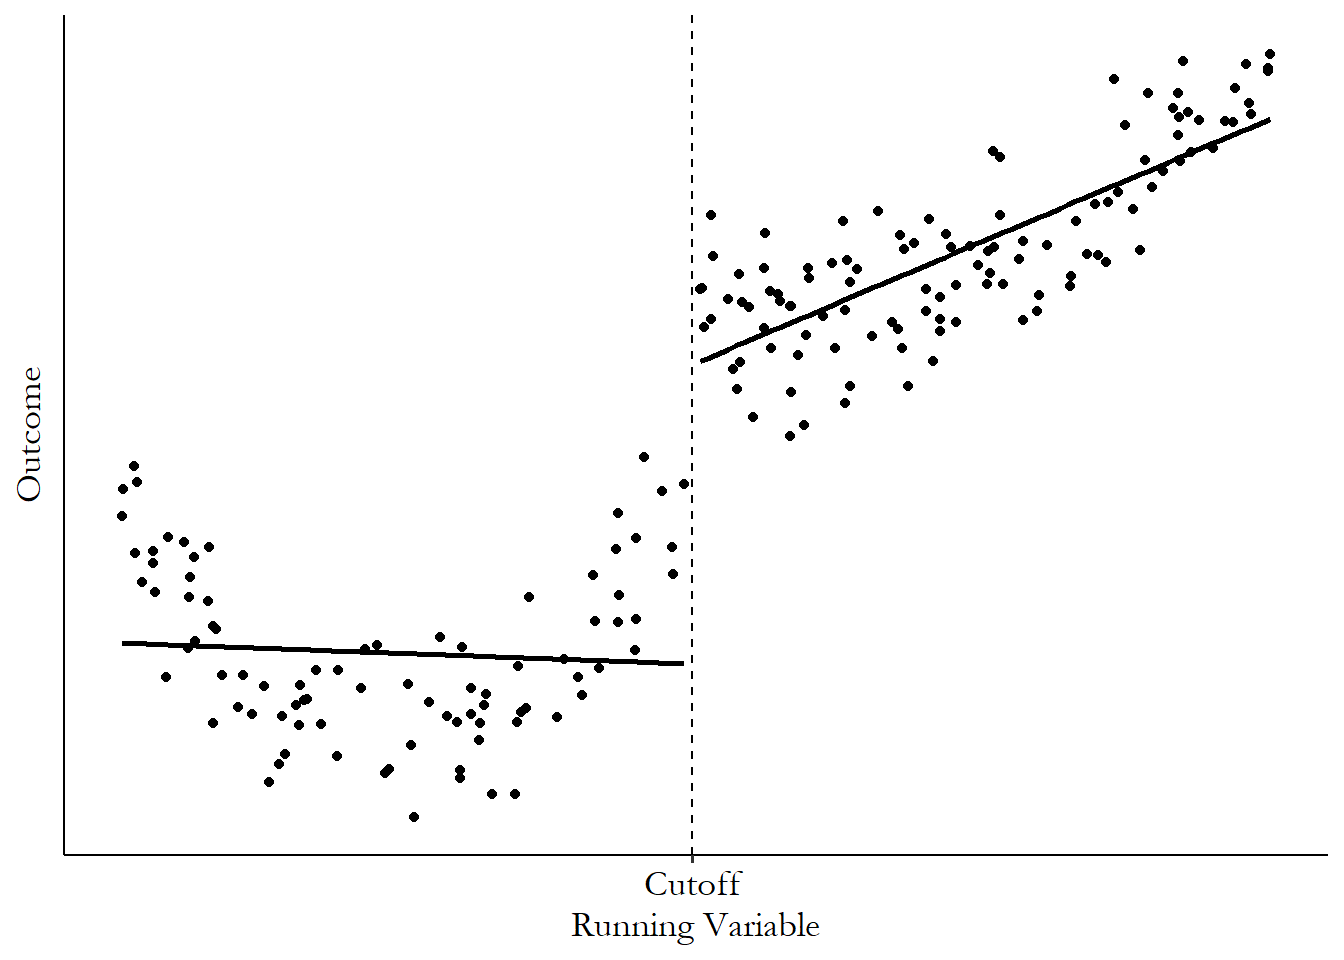
\includegraphics[width=0.85\textwidth]{figure/regressiondiscontinuity-linearrdd-1.png}
		\end{figure}
		\begin{minipage}{0.9\linewidth}
			\fontsize{8}{8pt}\selectfont
			\emph{Source:} Nick Huntington-Klein, The Effect: An Introduction to Research Design and Causality, Chapter 20
			
		\end{minipage}
	\end{center}
	
	
	
	
\end{frame}





\begin{frame}{Sharp RDD Estimation}{Parametric/Global Approach}
	\begin{itemize}
		\item To \textbf{estimate the discontinuity at cutoff}, we need to model the relationship between assignment variable $A$ and outcome $Y$
		\vspace{0.2cm}
		\item Suppose that potential outcomes can be described by some reasonably smooth function $\mathrm{f}(A_i)$:
		\begin{align*}
		E[\mathrm{Y}^{0}_{i}|A_i]=\beta+ \mathrm{f}(A_i) \\
		\mathrm{Y}^{1}_{i} = \mathrm{Y}^{0}_{i}+\alpha
		\end{align*}
		
		\item We can get RD estimates by fitting:
		\begin{equation*}
		Y_i=\beta +\alpha D_i+\mathrm{f}(A_i)+\eta_i
		\end{equation*}
		
	\end{itemize}
\end{frame}












\begin{frame}{Sharp RDD Estimation}{Parametric/Global Approach}
	\begin{itemize}
		
		\item Assume $\mathrm{f}(A_i)$ is a linear function of $A_{i}$
		\vspace{0.2cm}
		\item We usually do the following two settings:
		\vspace{0.2cm}
			\begin{itemize}
		\item[1] Allow the $A_i$ terms to differ on both sides of the threshold 
				\vspace{0.2cm}
			\begin{itemize}
			\item Include $A_{i}$ both individually and interacting them with $D_i$
			\vspace{0.2cm}
			\item By doing this, we can estimate $\mathrm{f}(A_i)$ on each side
						\vspace{0.2cm}
		\end{itemize}
			\item[2] Re-center $A_{i}$ at $c$: 
		\vspace{0.2cm}
		\begin{itemize}
			\item This step ensures that the treatment effect at $A_i=c$ is the coefficient on $D_i$ in a regression model 
		\end{itemize}
		
			\end{itemize}
	
	
		
		
		
		%\item The treatment effect (ATE) at $R=c$ is $\rho + \beta_1 c + \beta_2 c^{2} + ...+\beta_p c^p_i$
		%\vspace{0.2cm}
		
		
		
	\end{itemize}
\end{frame}










\begin{frame}{Sharp RDD Estimation}{Parametric/Global Approach}
	\begin{itemize}
		
		
		\item Therefore, we estimate the following regression model:
	
	\begin{equation*}
		Y_i = \beta +\alpha D_i+ \gamma_1 (A_{i}-c) + \gamma_2 (A_{i}-c) \times D_i +\eta_i
	\end{equation*}
		\vspace{0.2cm}
		\begin{itemize}
			
			\item The intercept at untreated side around the cutoff: $\beta$ 
			\vspace{0.2cm}
			\item The intercept at treated side around the cutoff: $\beta +\alpha$ 
			\vspace{0.2cm}
			\item The discontinuity in outcome at cutoff: $(\beta +\alpha)$ - $\beta$ = $\alpha$
						\vspace{0.2cm}
					\begin{itemize}
			\item $\alpha=\lim_{\varepsilon\rightarrow 0}\mathrm{E}[\mathrm{Y}_{i}|A_i=c+\varepsilon] - \lim_{\varepsilon\rightarrow 0}\mathrm{E}[\mathrm{Y}_{i}|A_i=c-\varepsilon]$
				\end{itemize}
			%The treatment effect (ATE) at $R=c$ is $\rho$
			%\vspace{0.2cm}
			%\item[3] The treatment effect (ATE) at $A_i-c=s>0$ is: \\$\rho+\beta^*_1 s+\beta^*_2 s^2+...+\beta^*_p s^p$
		\end{itemize}
		
	\end{itemize}
\end{frame}


\begin{frame}{More Flexible Function}
	
	
	\begin{center}
		\begin{figure}[p]
			\centering
			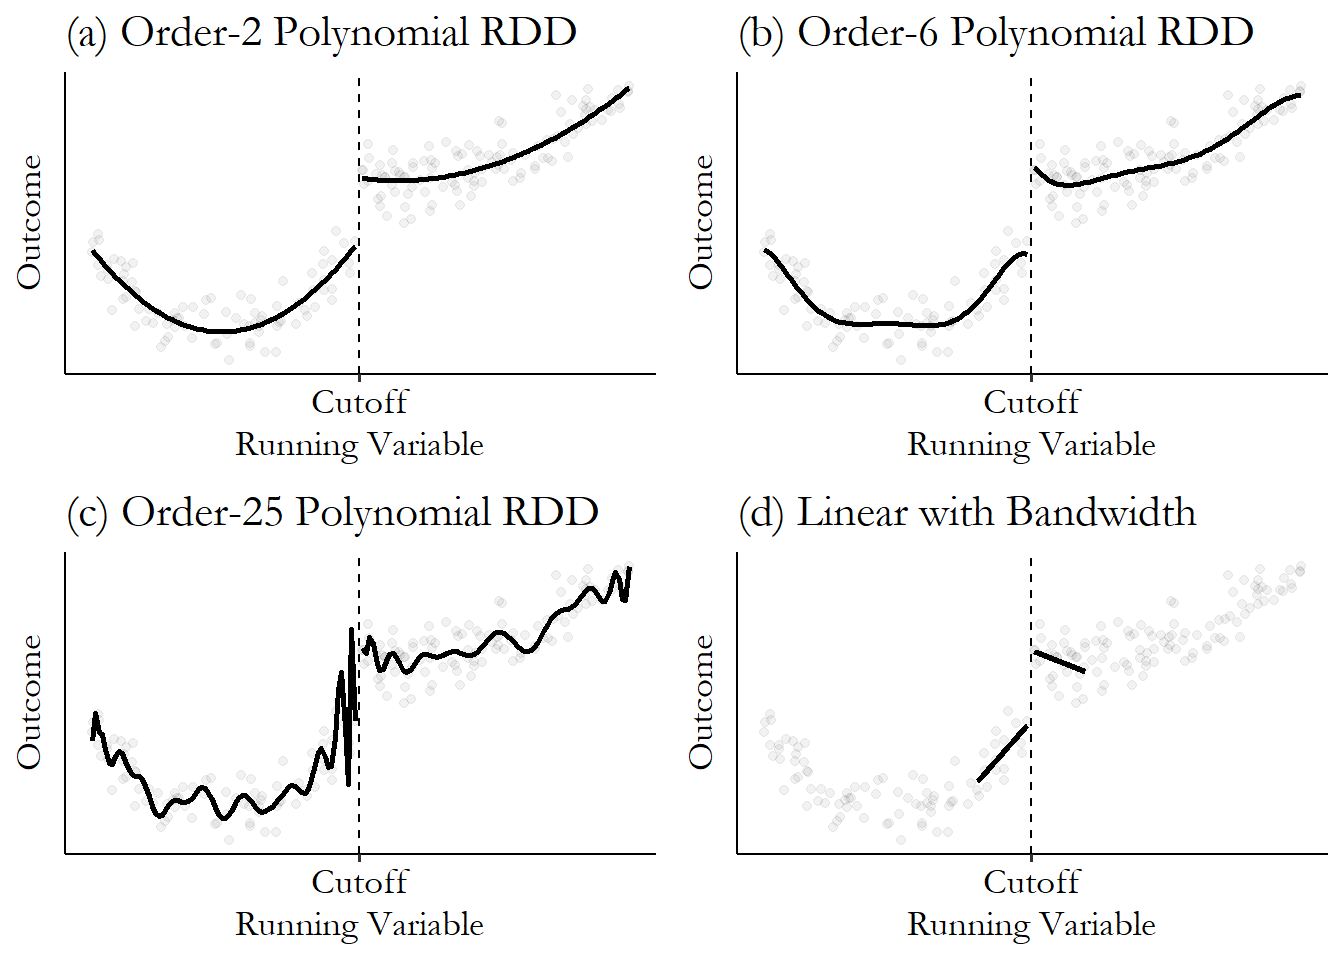
\includegraphics[width=0.85\textwidth]{figure/regressiondiscontinuity-poly-1.png}
		\end{figure}
		\begin{minipage}{0.9\linewidth}
			\fontsize{8}{8pt}\selectfont
			\emph{Source:} Nick Huntington-Klein, The Effect: An Introduction to Research Design and Causality, Chapter 20
			
		\end{minipage}
	\end{center}
	
	
	
	
\end{frame}




\begin{frame}{Sharp RDD Estimation}{Parametric/Global Approach}
	\begin{itemize}
		
		
		
		\item We can use more flexible function $\mathrm{f}(A_i)$ to capture the relationship between assignment variable $A$ and outcome $Y$
									\vspace{0.2cm}
			\begin{itemize}
			\item For example, use second-order polynomial of $A$
							\vspace{0.2cm}
		\item However, more flexible function $\mathrm{f}(A_i)$ might not give better estimate of discontinuity  
					\vspace{0.2cm}
				\end{itemize}		
		\item Gelman and Imbens (2019): 
							\vspace{0.2cm}
			\begin{itemize}
		\item It's not a great idea to go above the second-order term when performing RDD
						\vspace{0.2cm}
	
	\item If there's a complex shape that needs fitting, instead try limiting the range of the data with a bandwidth and use a simpler function
		\end{itemize}
	\end{itemize}
\end{frame}














\begin{frame}{Sharp RDD Estimation}{Nonparametric/Local Approach}
	\begin{itemize}

		\item The core idea of RDD is to compare outcomes just above and just below the cutoff $c$.
		\vspace{0.2cm}
		\item Nonparametric/local method:
		\vspace{0.2cm}
		\begin{itemize}
			\item We do \textbf{not} assume a specific global functional form for the relationship between the outcome $Y$ and the assignment variable $A$ over their entire range. 
						\vspace{0.2cm}
					\begin{itemize}
			\item This is what "nonparametric" means in this context.
			\vspace{0.2cm}
					\end{itemize}
			\item Instead, we focus the analysis \textbf{locally}, using only observations close to the cutoff $c$.
			\vspace{0.2cm}
			\item We compare treated and untreated observations that fall within a specific \textbf{bandwidth ($h$)} around the cutoff.
		\end{itemize}
		
	\end{itemize}
		
		

\end{frame}






\begin{frame}{Sharp RDD Estimation}{Nonparametric/Local Approach}
\begin{itemize}
	%\item As mentioned, the "nonparametric" aspect means we avoid assuming a global functional form for $E[Y_i | A_i = a]$.
	%\vspace{0.2cm}
	%\item However, we still need a way to estimate the potential jump in $Y$ precisely *at* the cutoff $c$.
	%\vspace{0.2cm}
	\item Key insight: within a \textbf{sufficiently small local window (bandwidth $h$)} around the cutoff $c$, even if the true relationship is complex globally.
	\begin{itemize}
		\vspace{0.2cm}
	\item It can often be well \textbf{approximated by a simple linear function}.
	\vspace{0.2cm}
\end{itemize}
	\item Therefore, we use \textbf{Local linear regression}:
			\vspace{0.2cm}
	\begin{itemize}
		\item This involves fitting separate linear regressions on each side of the cutoff, but \textit{only} using data within the bandwidth $h$.
		\vspace{0.2cm}
		%\item This allows for different intercepts and slopes on either side of $c$.
		%\vspace{0.2cm}
		\item Optionally, kernel functions can be used to give more weight to observations closer to the cutoff.
	\end{itemize}
%	\item This approach is generally preferred over simply comparing means in bins next to the cutoff, as it helps reduce potential bias near the boundary of the bandwidth.
\end{itemize}
\end{frame}





\begin{frame}{Sharp RDD Estimation}{Implementing Local Linear Regression}
	\begin{itemize}
		\item Specifically, we estimate the following regression model \textbf{using only observations within the chosen bandwidth $h$}:
		\begin{equation*}
			Y_i = \beta +\alpha D_i+ \gamma_1 (A_{i}-c) + \gamma_2 (A_{i}-c) \times D_i +\eta_i
		\end{equation*}
		\item This linear model is just a \textbf{local approximation} of the relationship near the cutoff $c$, within the bandwidth $h$. 
				\vspace{0.2cm}
			\begin{itemize}
		\item It is \textit{not} a global assumption about the functional form.
		\vspace{0.2cm}
			\end{itemize}
%		\item Interpretation of coefficients:
%		\begin{itemize}
%			\item $D_i$: Treatment indicator (=1 if $A_i \ge c$, 0 if $A_i < c$).
%			\item $A_i - c$: Assignment variable centered at the cutoff.
%			\item $\beta$: The estimated intercept for the control group ($D_i=0$) at the cutoff ($A_i = c$).
%			\item $\alpha$: \textbf{The RDD Treatment Effect}. This estimates the jump (discontinuity) in the outcome $Y$ at the cutoff $c$ comparing the treated ($D_i=1$) to the control ($D_i=0$) group. \textbf{This is the parameter of primary interest.}
%			\item $\gamma_1$: The estimated slope of the relationship between $Y$ and $(A_i-c)$ for the control group ($D_i=0$) within the bandwidth.
%			\item $\gamma_2$: The estimated \textit{change} in slope for the treated group ($D_i=1$) compared to the control group, within the bandwidth. (The slope for the treated group is $\gamma_1 + \gamma_2$).
%		\end{itemize}
		\item The estimated coefficient $\hat{\alpha}$ provides the RDD estimate of the treatment effect.
	\end{itemize}
\end{frame}









\begin{frame}{Bandwidth}
	
	
	\begin{center}
		\begin{figure}[p]
			\centering
			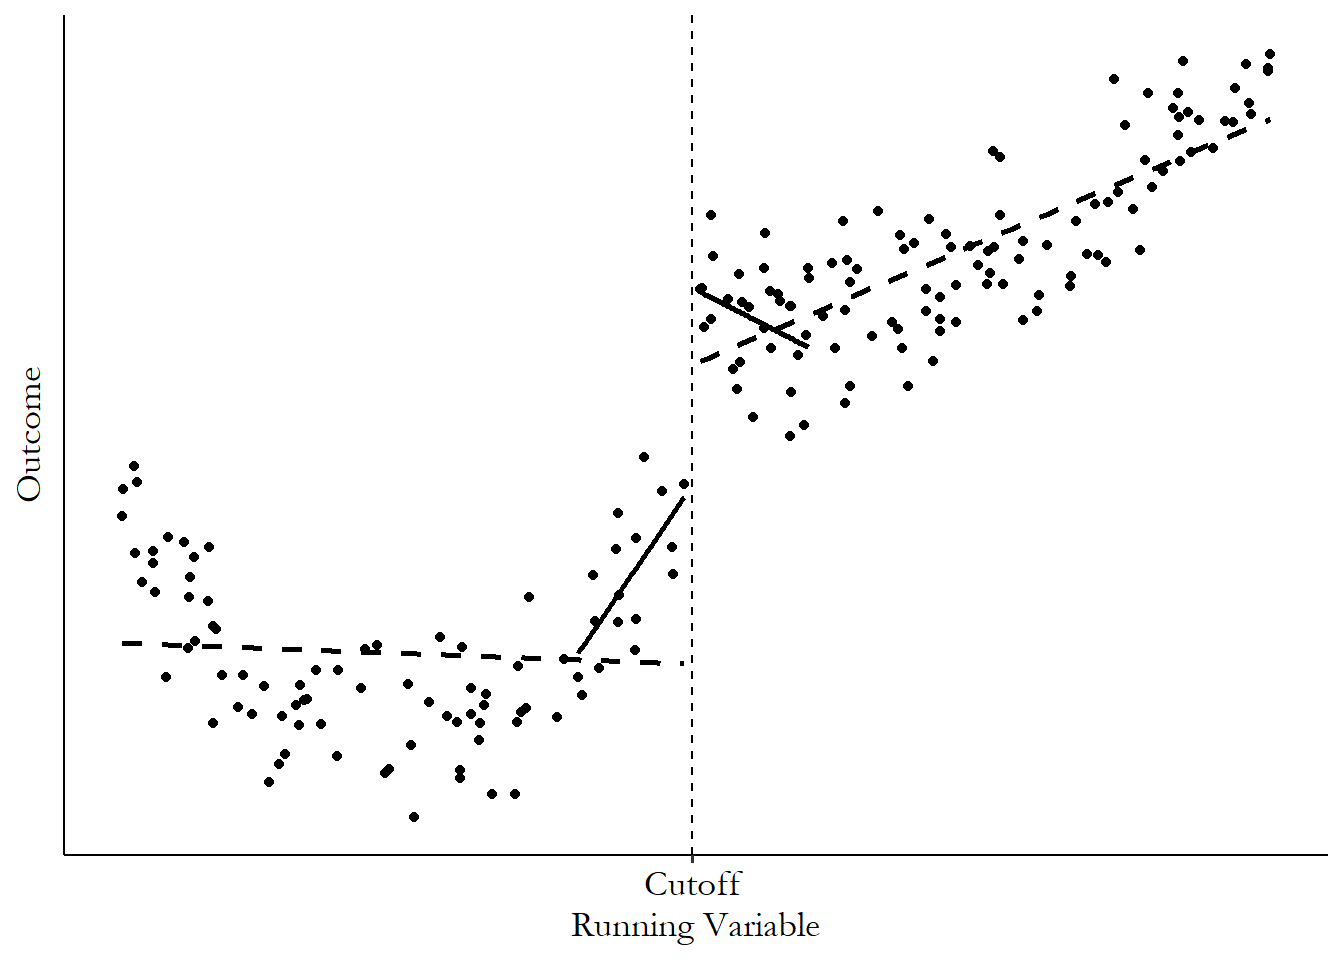
\includegraphics[width=0.85\textwidth]{figure/regressiondiscontinuity-localproblems-1.png}
		\end{figure}
		\begin{minipage}{0.9\linewidth}
			\fontsize{8}{8pt}\selectfont
			\emph{Source:} Nick Huntington-Klein, The Effect: An Introduction to Research Design and Causality, Chapter 20
			
		\end{minipage}
	\end{center}
	
	
	
	
\end{frame}


\begin{frame}{Sharp RDD Estimation}{Nonparametric/Local Approach}
	\begin{itemize}
		\item The main challenge of nonparametric approach is to \textbf{choose a bandwidth} 
		\vspace{0.2cm}
		\item There is essentially a trade-off between \textbf{bias} and \textbf{precision} (efficiency) 
		\vspace{0.2cm}
		\item Use a larger bandwidth:  
		\vspace{0.2cm}
		\begin{itemize}
			\item Since more data points are used in the regression
			\vspace{0.2cm}	
			\item Get more \textbf{precise} treatment effect estimates
			\vspace{0.2cm}
			\item But use data points far from cutoff 
			\vspace{0.2cm}
			%\item Linear specification is less likely to be accurate
			%\vspace{0.2cm}
			\item The estimated treatment effect could be \textbf{biased}
		\end{itemize}
		
		
	\end{itemize}
\end{frame}





\begin{frame}{Sharp RDD Estimation}{How to Choose Bandwidth}
	\begin{itemize}
		\item[1.] \textbf{Cross-Validation (CV) Procedure}:
		\vspace{0.2cm}
		\begin{itemize}
			\item Aims to select $h$ that minimizes prediction errors of the RDD model specifically in the neighborhood of the cutoff $c$.
			%\vspace{0.2cm}
			%\item This often involves minimizing a cross-validated criterion, such as the sum of squared residuals, derived from local polynomial RDD model fits.
		\end{itemize}
		\vspace{0.3cm} % Adjusted spacing for clarity
		\item[2.] \textbf{Plug-In Procedure}:
		\vspace{0.2cm}
		\begin{itemize}
			\item Derives a formula for the optimal bandwidth ($h_{opt}$) by analytically minimizing an (Asymptotic) Mean Squared Error for the RDD treatment effect estimator (e.g., $\hat{\alpha}$)
			
			%expression for the RDD treatment effect estimator (e.g., $\hat{\alpha}$).
			\vspace{0.2cm}
			\begin{itemize}
				%\item This AMSE typically reflects a trade-off between the squared bias and the variance of the estimator.
				%\vspace{0.2cm}
				\item The $h_{opt}$ formula depends on some unknown data characteristics at the cutoff $c$ (like local trends and data variability). 
				\vspace{0.2cm}
				\item These must first be estimated from your data, often using a "pilot" bandwidth.
				\vspace{0.2cm}
			\end{itemize}		
			\item See, e.g., Imbens and Kalyanaraman (2012), Calonico, Cattaneo, and Titiunik (2014).
		\end{itemize}
	\end{itemize}
\end{frame}




\begin{frame}{Sharp RDD Estimation}{Nonparametric/Local Approach}
	\begin{itemize}
		\item In practice, we also use a specific kernel function to weight observations more heavily around cutoff
		
					\vspace{0.2cm}
		\item A very commonly-used kernel in regression discontinuity is the \textbf{triangular kernel}
		
\begin{equation}
	K(A) = 
	\begin{cases} 
		1 - \frac{\left| A_{i} - c \right|}{h} & \text{for}\: c - h < A_{i} < c + h, \\
		0 & \text{otherwise.}
	\end{cases}
\end{equation}

%Therefore, we estimate the following local linear regression
		
	\end{itemize}
\end{frame}


\begin{frame}{Triangular Kernel Function}
	
	
	\begin{center}
		\begin{figure}[p]
			\centering
			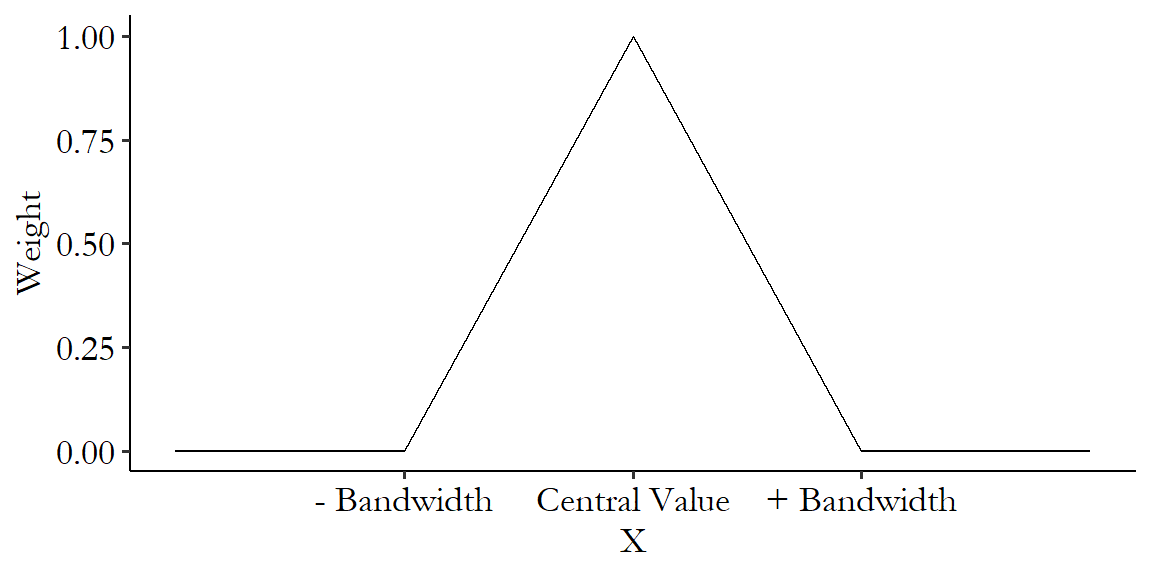
\includegraphics[width=0.9\textwidth]{figure/regressiondiscontinuity-kernel-1.png}
		\end{figure}
		\begin{minipage}{0.9\linewidth}
			\fontsize{8}{8pt}\selectfont
			\emph{Source:} Nick Huntington-Klein, The Effect: An Introduction to Research Design and Causality, Chapter 20
			
		\end{minipage}
	\end{center}
	
	
	
	
\end{frame}




%\begin{frame}{Sharp RDD Estimation}{Nonparametric/Local Approach}
%	\begin{itemize}
%		%\item The standard solution to reduce this bias is to run \textbf{local linear regression}
%		%\vspace{0.2cm}
%		\item Therefore, we estimate the following local linear regression 
%		\begin{equation*}
%			Y_i = \beta +\alpha D_i+ \gamma_1 (A_{i}-c) + \gamma_2 (A_{i}-c) \times D_i +\eta_i
%		\end{equation*}
%		
%			\begin{itemize}
%		\item Within a given window of width $h$ around the cutoff
%		\vspace{0.2cm}
%		\item Use a triangular kernel as a weight
%		\vspace{0.2cm}
%		\item Implement a weighted OLS
%			\end{itemize}
%	\end{itemize}
%\end{frame}




\begin{frame}{Sharp RDD Estimation}{Nonparametric/Local Approach}
	\begin{itemize}
		
		
		\item In alcohol example, we can estimate the following regression \textbf{within 180 days before and after age 21}:
		\begin{multline*}
		Y_i=\beta+\alpha D_{i}+\gamma_{1}(A_{i}-21) +\gamma_{2}D_{i}(A_{i}-21)+\eta_i 
		\end{multline*}
	\begin{itemize}		
		\item $h=180$
		\vspace{0.2cm}	
		\item Use a triangular kernel as a weight and implement a weighted OLS
		\vspace{0.2cm}
		\item The effect of legal access to alcohol on mortality rate at age 21 is $\alpha$
		\vspace{0.2cm}
		\item Usually, we would present the RD estimates by different choices of bandwidth
		\vspace{0.2cm}	
			\end{itemize}
	\end{itemize}
\end{frame}




\begin{frame}{}
	
	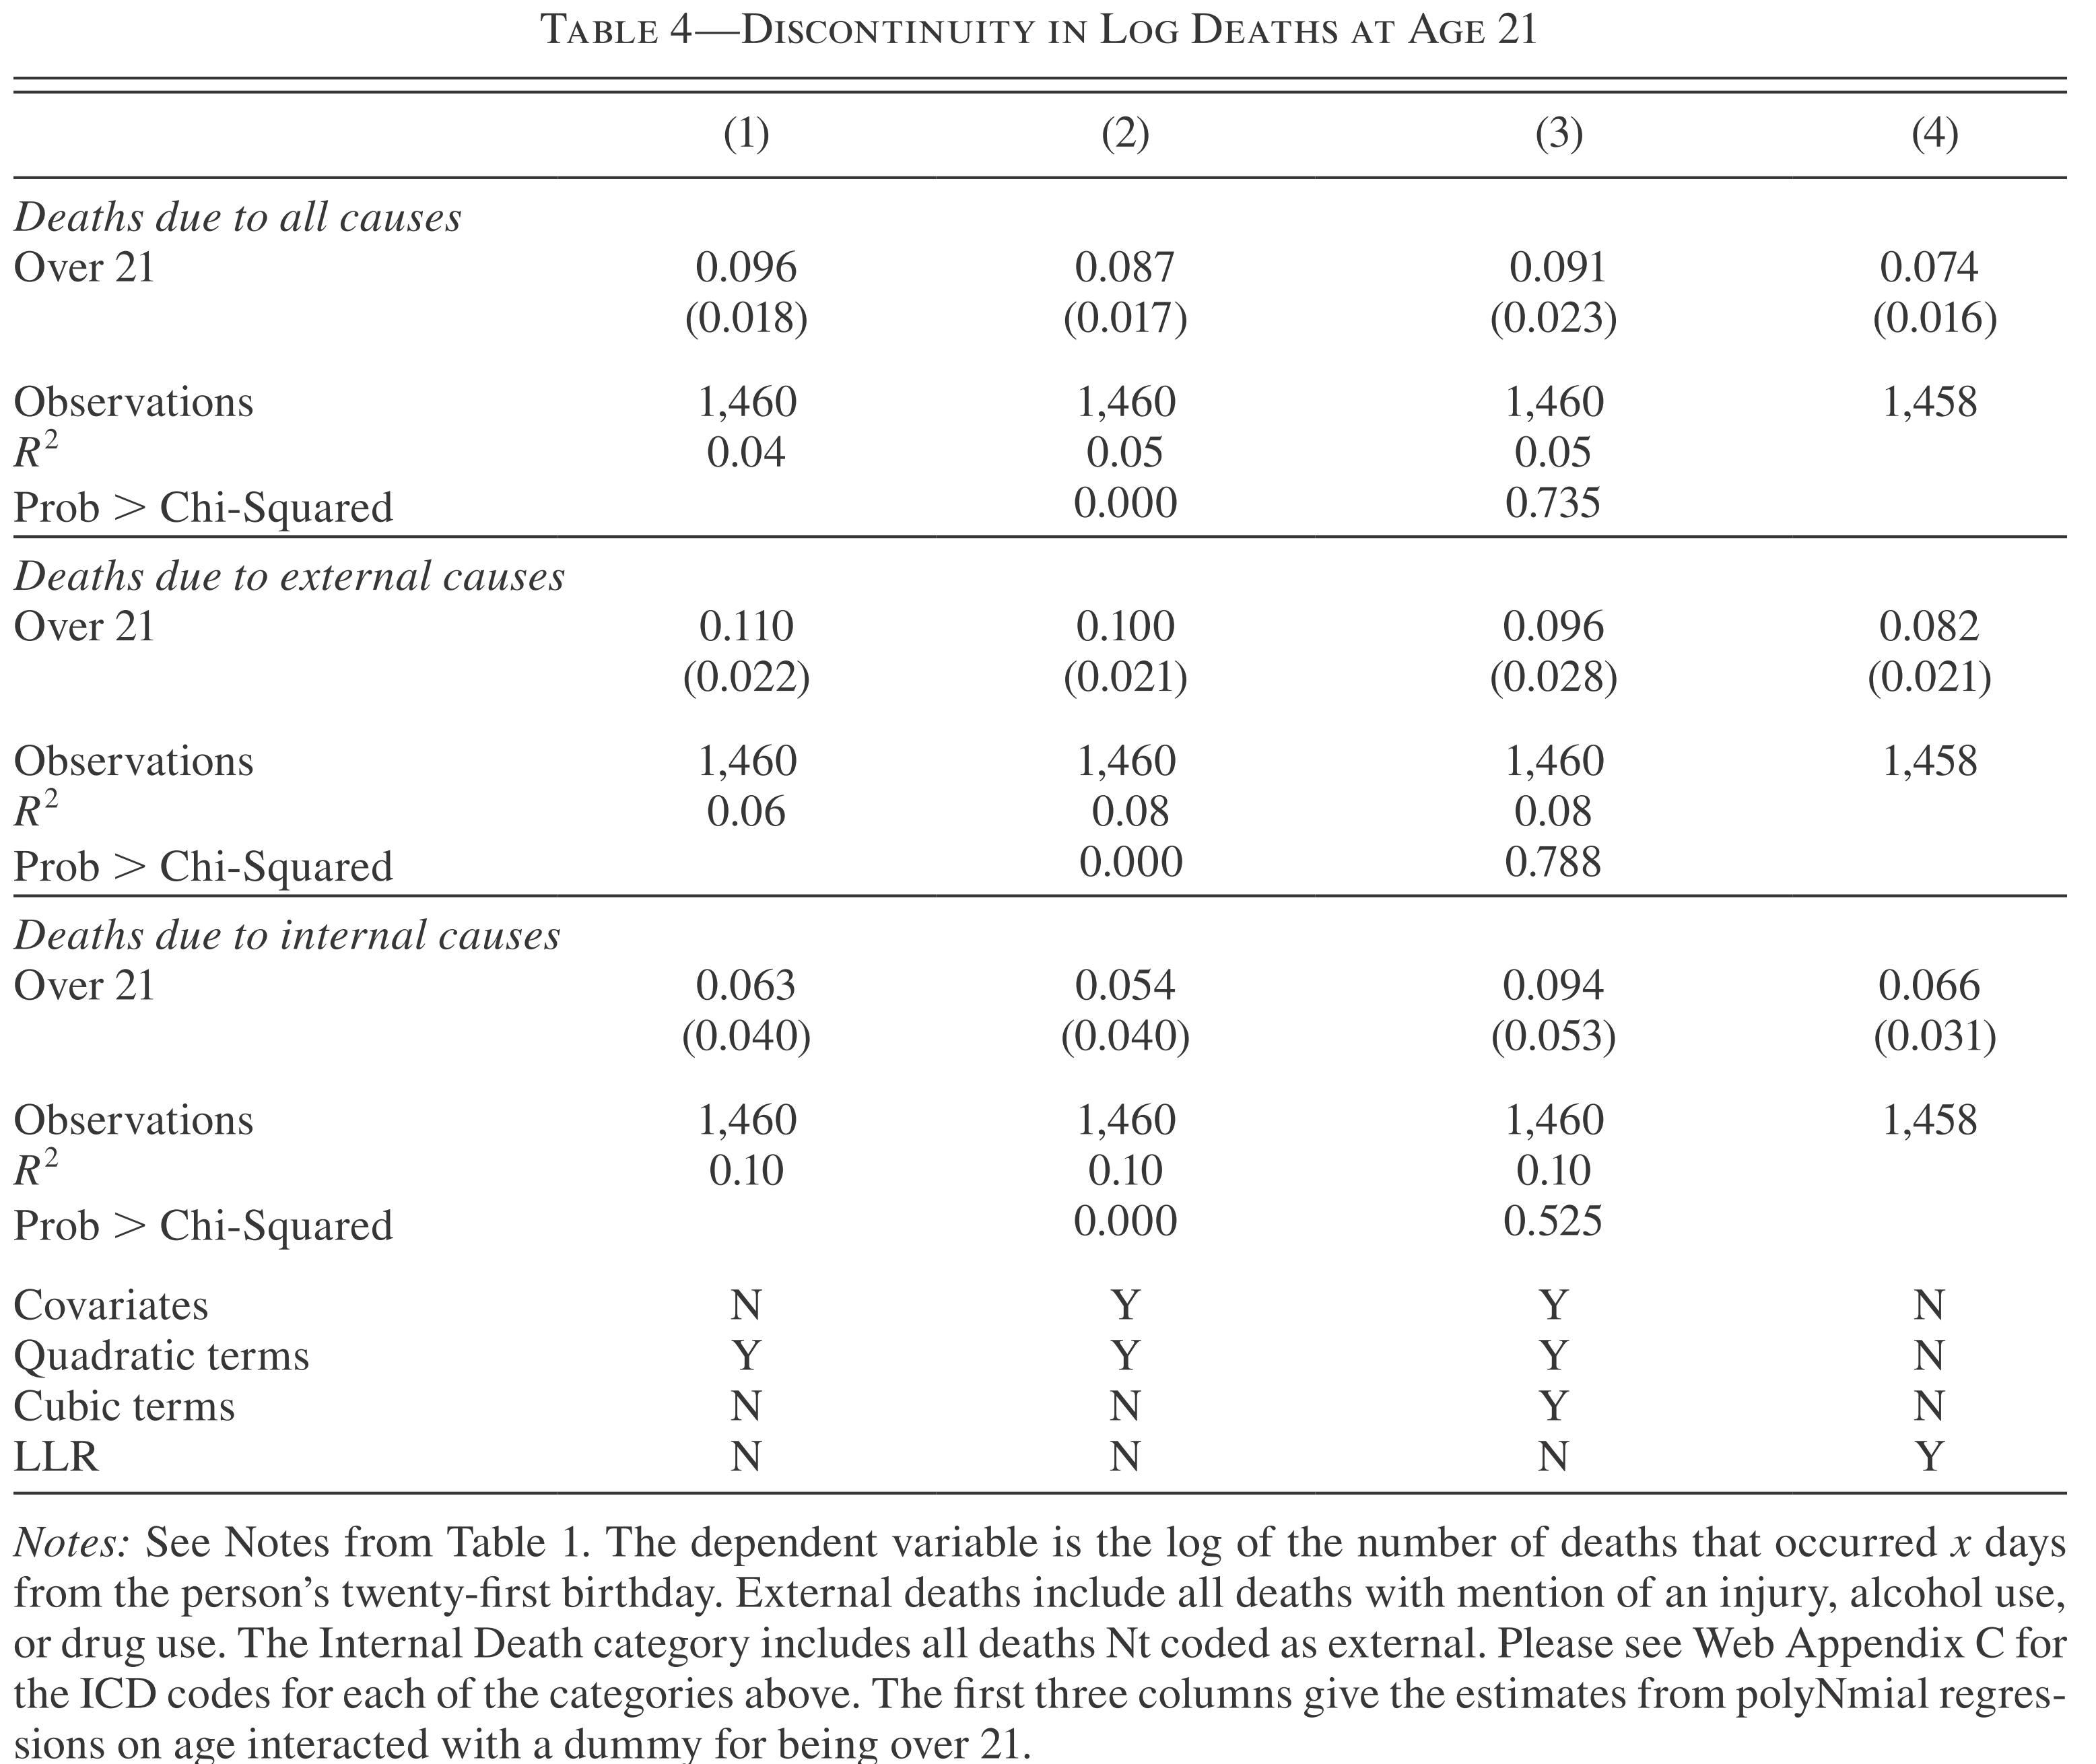
\includegraphics[width=0.9\textwidth]{figure/RD_drink_t4.jpg}
	
	
\end{frame}



\begin{frame}{}
	
	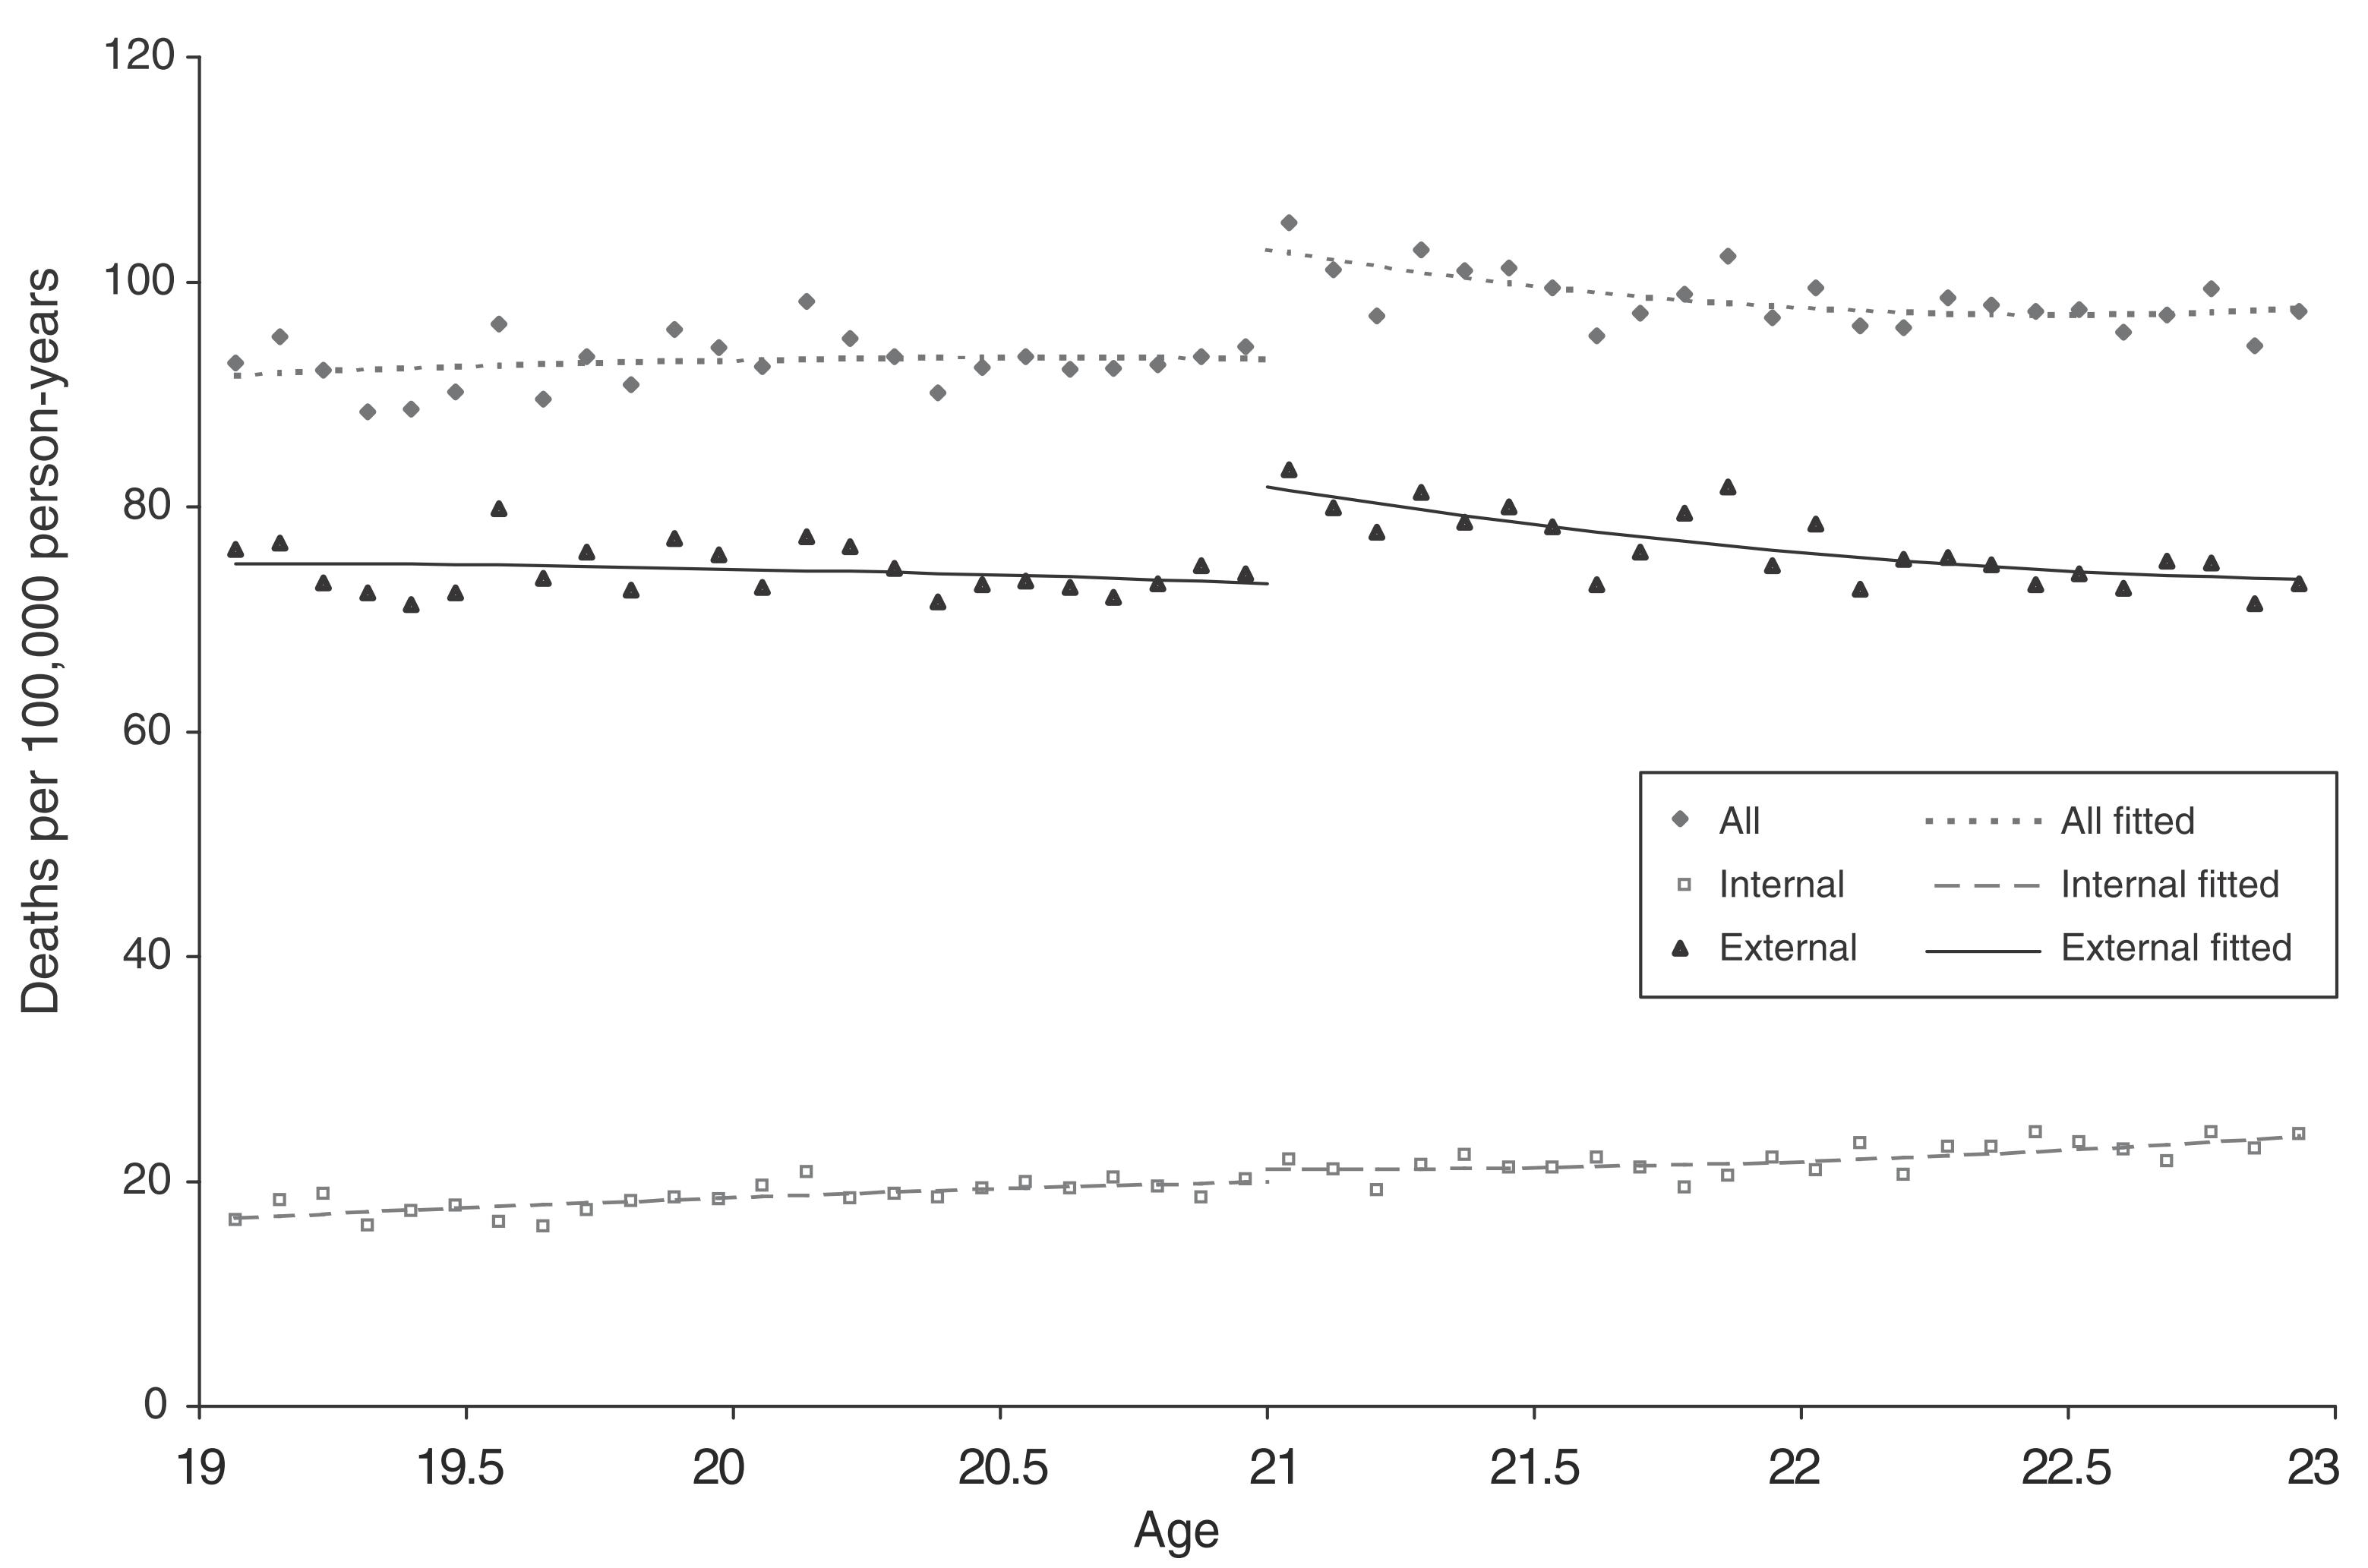
\includegraphics[width=0.9\textwidth]{figure/alcohol_f1.jpg}
	
	
\end{frame}



\begin{frame}{}
	
	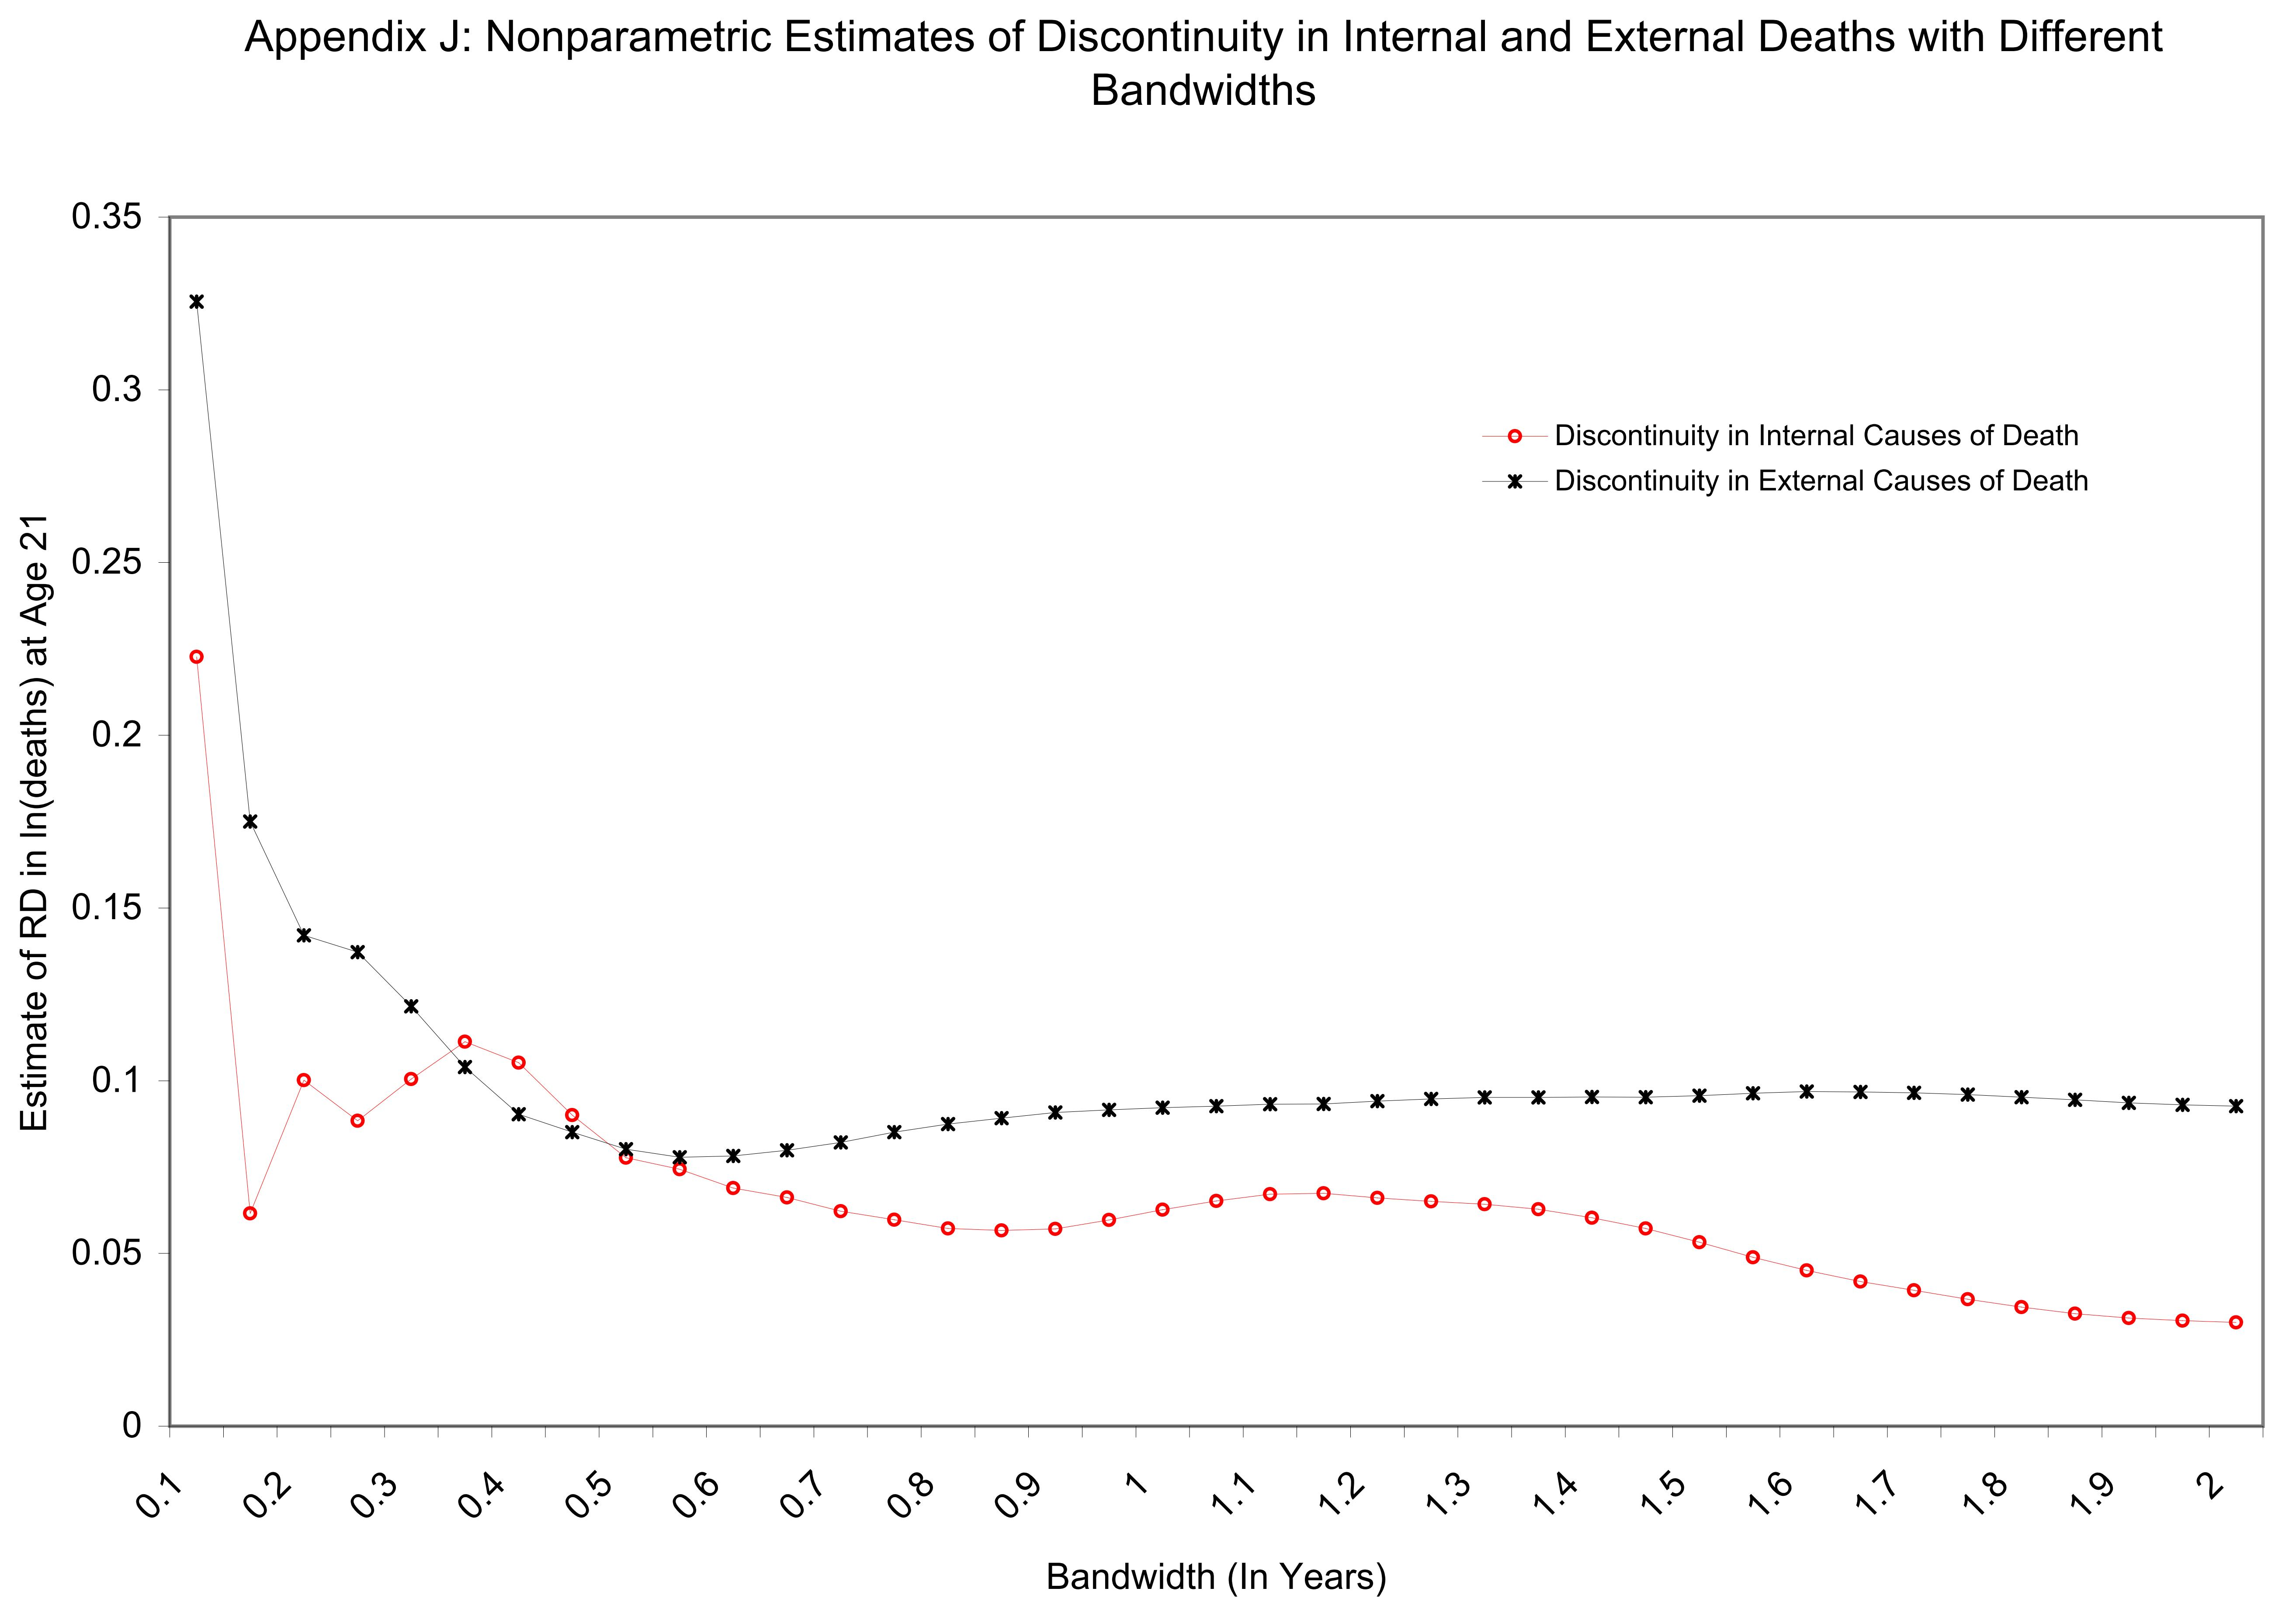
\includegraphics[width=1.0\textwidth]{figure/RD_drink_f5.jpg}
	
	
\end{frame}




	






%\begin{frame}{Sharp RDD Estimation}{How to Choose Bandwidth}
%	\begin{itemize}
%		\item[1] \textbf{Cross-Validation Procedure}: 
%		\vspace{0.2cm}
%		\begin{itemize}
%			\item Choose bandwidth $h$ that produces the best fit for
%			the relationship of outcome and assignment variable
%			\vspace{0.2cm}
%		\end{itemize}
%		\vspace{0.2cm}
%		\item[2] \textbf{Plug-In Procedure}: 
%		\vspace{0.2cm}
%		\begin{itemize} 
%			\item Solve for the optimal bandwidth formula in terms of minimizing mean square error
%			
%			\vspace{0.2cm}
%			\item Plug the parameters into formula to get optimal bandwidth
%			\vspace{0.2cm}
%			\item  See, e.g. Imbens and Kalyanaraman (2009), Calonico, Cattaneo, and Titiunik (2014)
%		\end{itemize}
%	\end{itemize}
%\end{frame}
%




\title[]  
{Examine Validity of Identification Assumptions}


\author 
{}

%\institute{Institute of Economics, Academia Sinica  \\ Econ, NTU}
%\institute{Institute of Economics, Academia Sinica  \\ IMES/IDAS, NTU}
\institute{}

%\author 
%{楊子霆 \\ 中研院經濟所}

%\institute 
%{中正大學國際經濟專題研討}




\date
{}


\begin{frame}{}
	\titlepage
\end{frame}




\begin{frame}{Test Internal Validity of RDD}{Examine ``Discontinuity" in Nonoutcome Variables}
	
	\textbf{1. Examine ``Discontinuity" in Nonoutcome Variables}
	
	\begin{itemize}
		\vspace{0.2cm}	
		\item Construct a similar graph to the one before but using a covariate as the ``outcome"
		\vspace{0.2cm}	
		\item There should be \textbf{NO jump in other covariates}
		\vspace{0.2cm}	
		\item If the covariates would jump at the cutoff one would doubt the identifying assumption
		
	\end{itemize}
\end{frame}




\begin{frame}{Test Internal Validity of RDD}{Sorting Behavior}
	
	\textbf{2. Examine ``Discontinuity" in Density of the assignment variable}
	
	\begin{itemize}
		\vspace{0.2cm}	
		\item Individuals may invalidate the \textbf{continuity assumption} if they strategically manipulate assignment variable $A$ to be just above or below the cutoff
		\vspace{0.2cm}
		\item That is, people just above and just below the cutoff are no longer comparable
		\vspace{0.2cm}
		
		
	\end{itemize}
\end{frame}



\begin{frame}{Consequence of Sorting Behavior}{Example}
	
	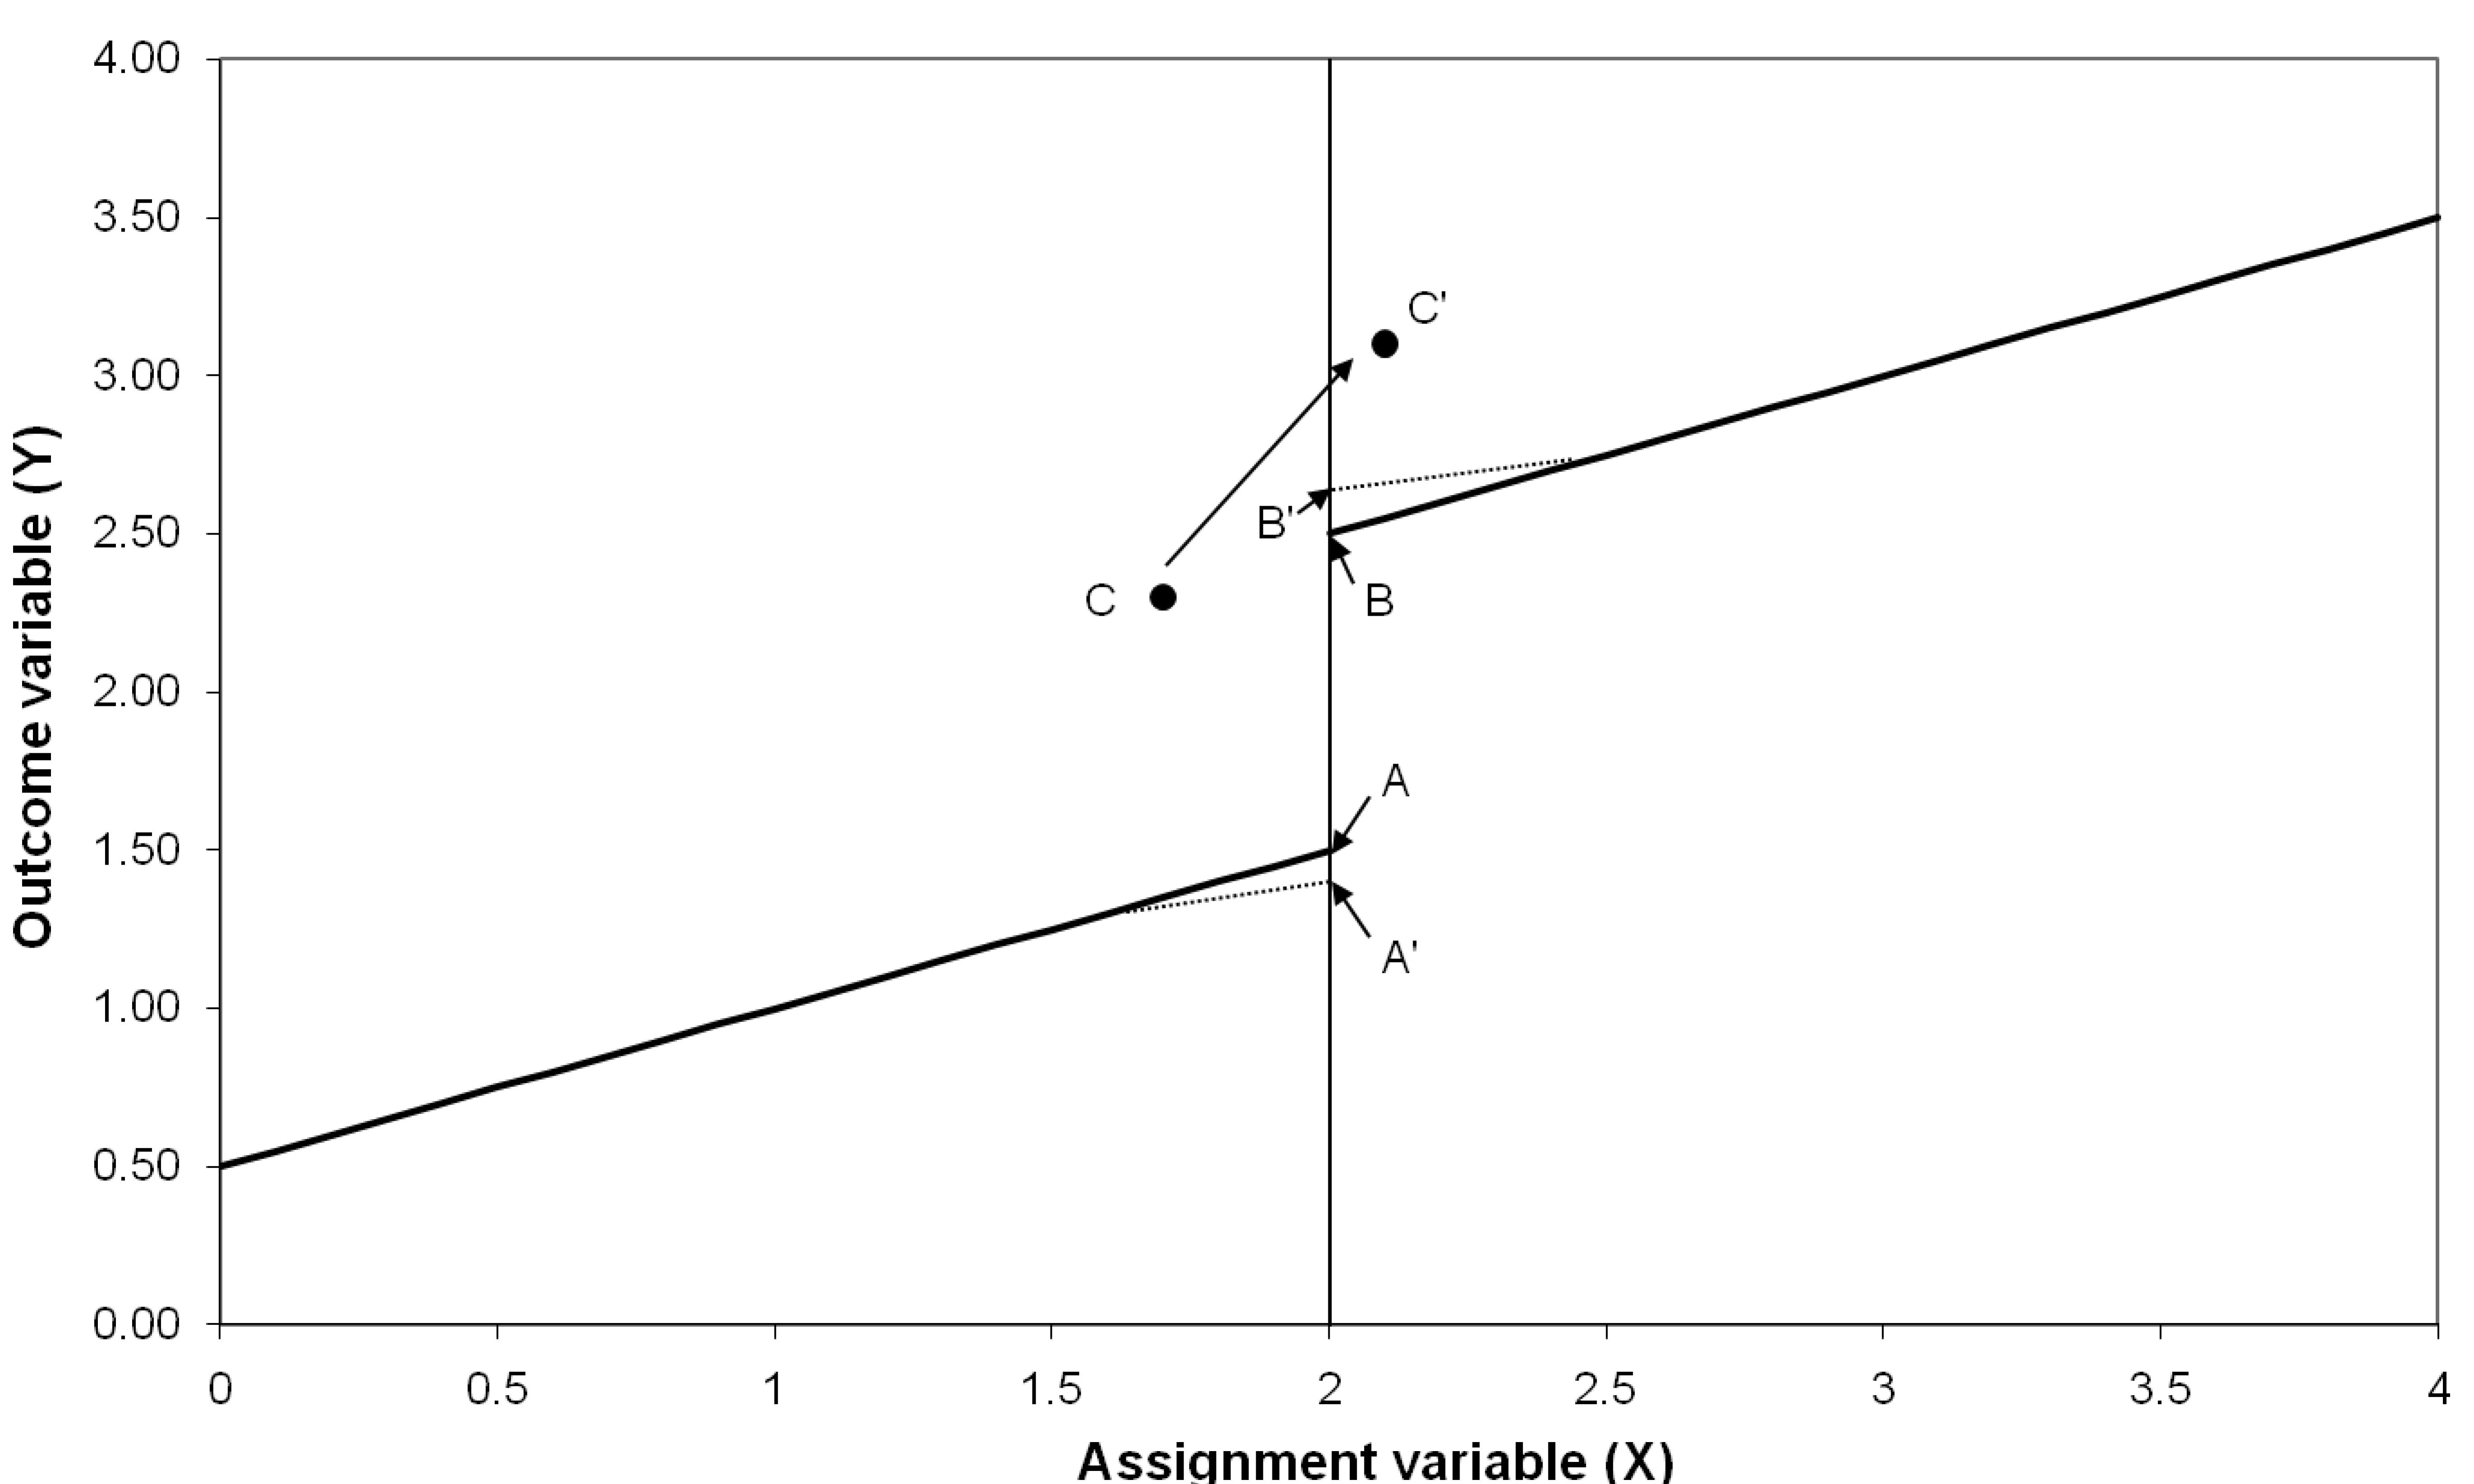
\includegraphics[width=1.0\textwidth]{figure/manu_f1.jpg}
	
	
\end{frame}



\begin{frame}{Sorting Behavior}{Example}
	\begin{itemize}
		
		\item This is a concern especially if the exact value of the cutoff is known to the individuals in advance
		\vspace{0.2cm}
			\begin{itemize}
		\item Such sorting behavior may create a \textbf{discontinuity in the distribution of $A$ at the cutoff}
		\vspace{0.2cm}
		\item That is, ``bunching" to the right or to the left of the cutoff
			\end{itemize}
	\end{itemize}
	
\end{frame}




\begin{frame}{Sorting Behavior}{Example}
	
	Adriana Camacho and Emily Conover (2011) ``\textbf{Manipulation of Social Program Eligibility}" AEJ: Economic Policy
			\vspace{0.2cm}
	\begin{itemize}
		\item Manipulation of a poverty index in Colombia
		\vspace{0.2cm}
			\begin{itemize}
		\item A poverty index is used to decide eligibility for social programs 
		\vspace{0.2cm}
			\end{itemize}
		\item The algorithm to create the poverty index \textbf{becomes public} during the second half of 1997
	\end{itemize}
\end{frame}




\begin{frame}{Sorting Behavior}{Example}
	
	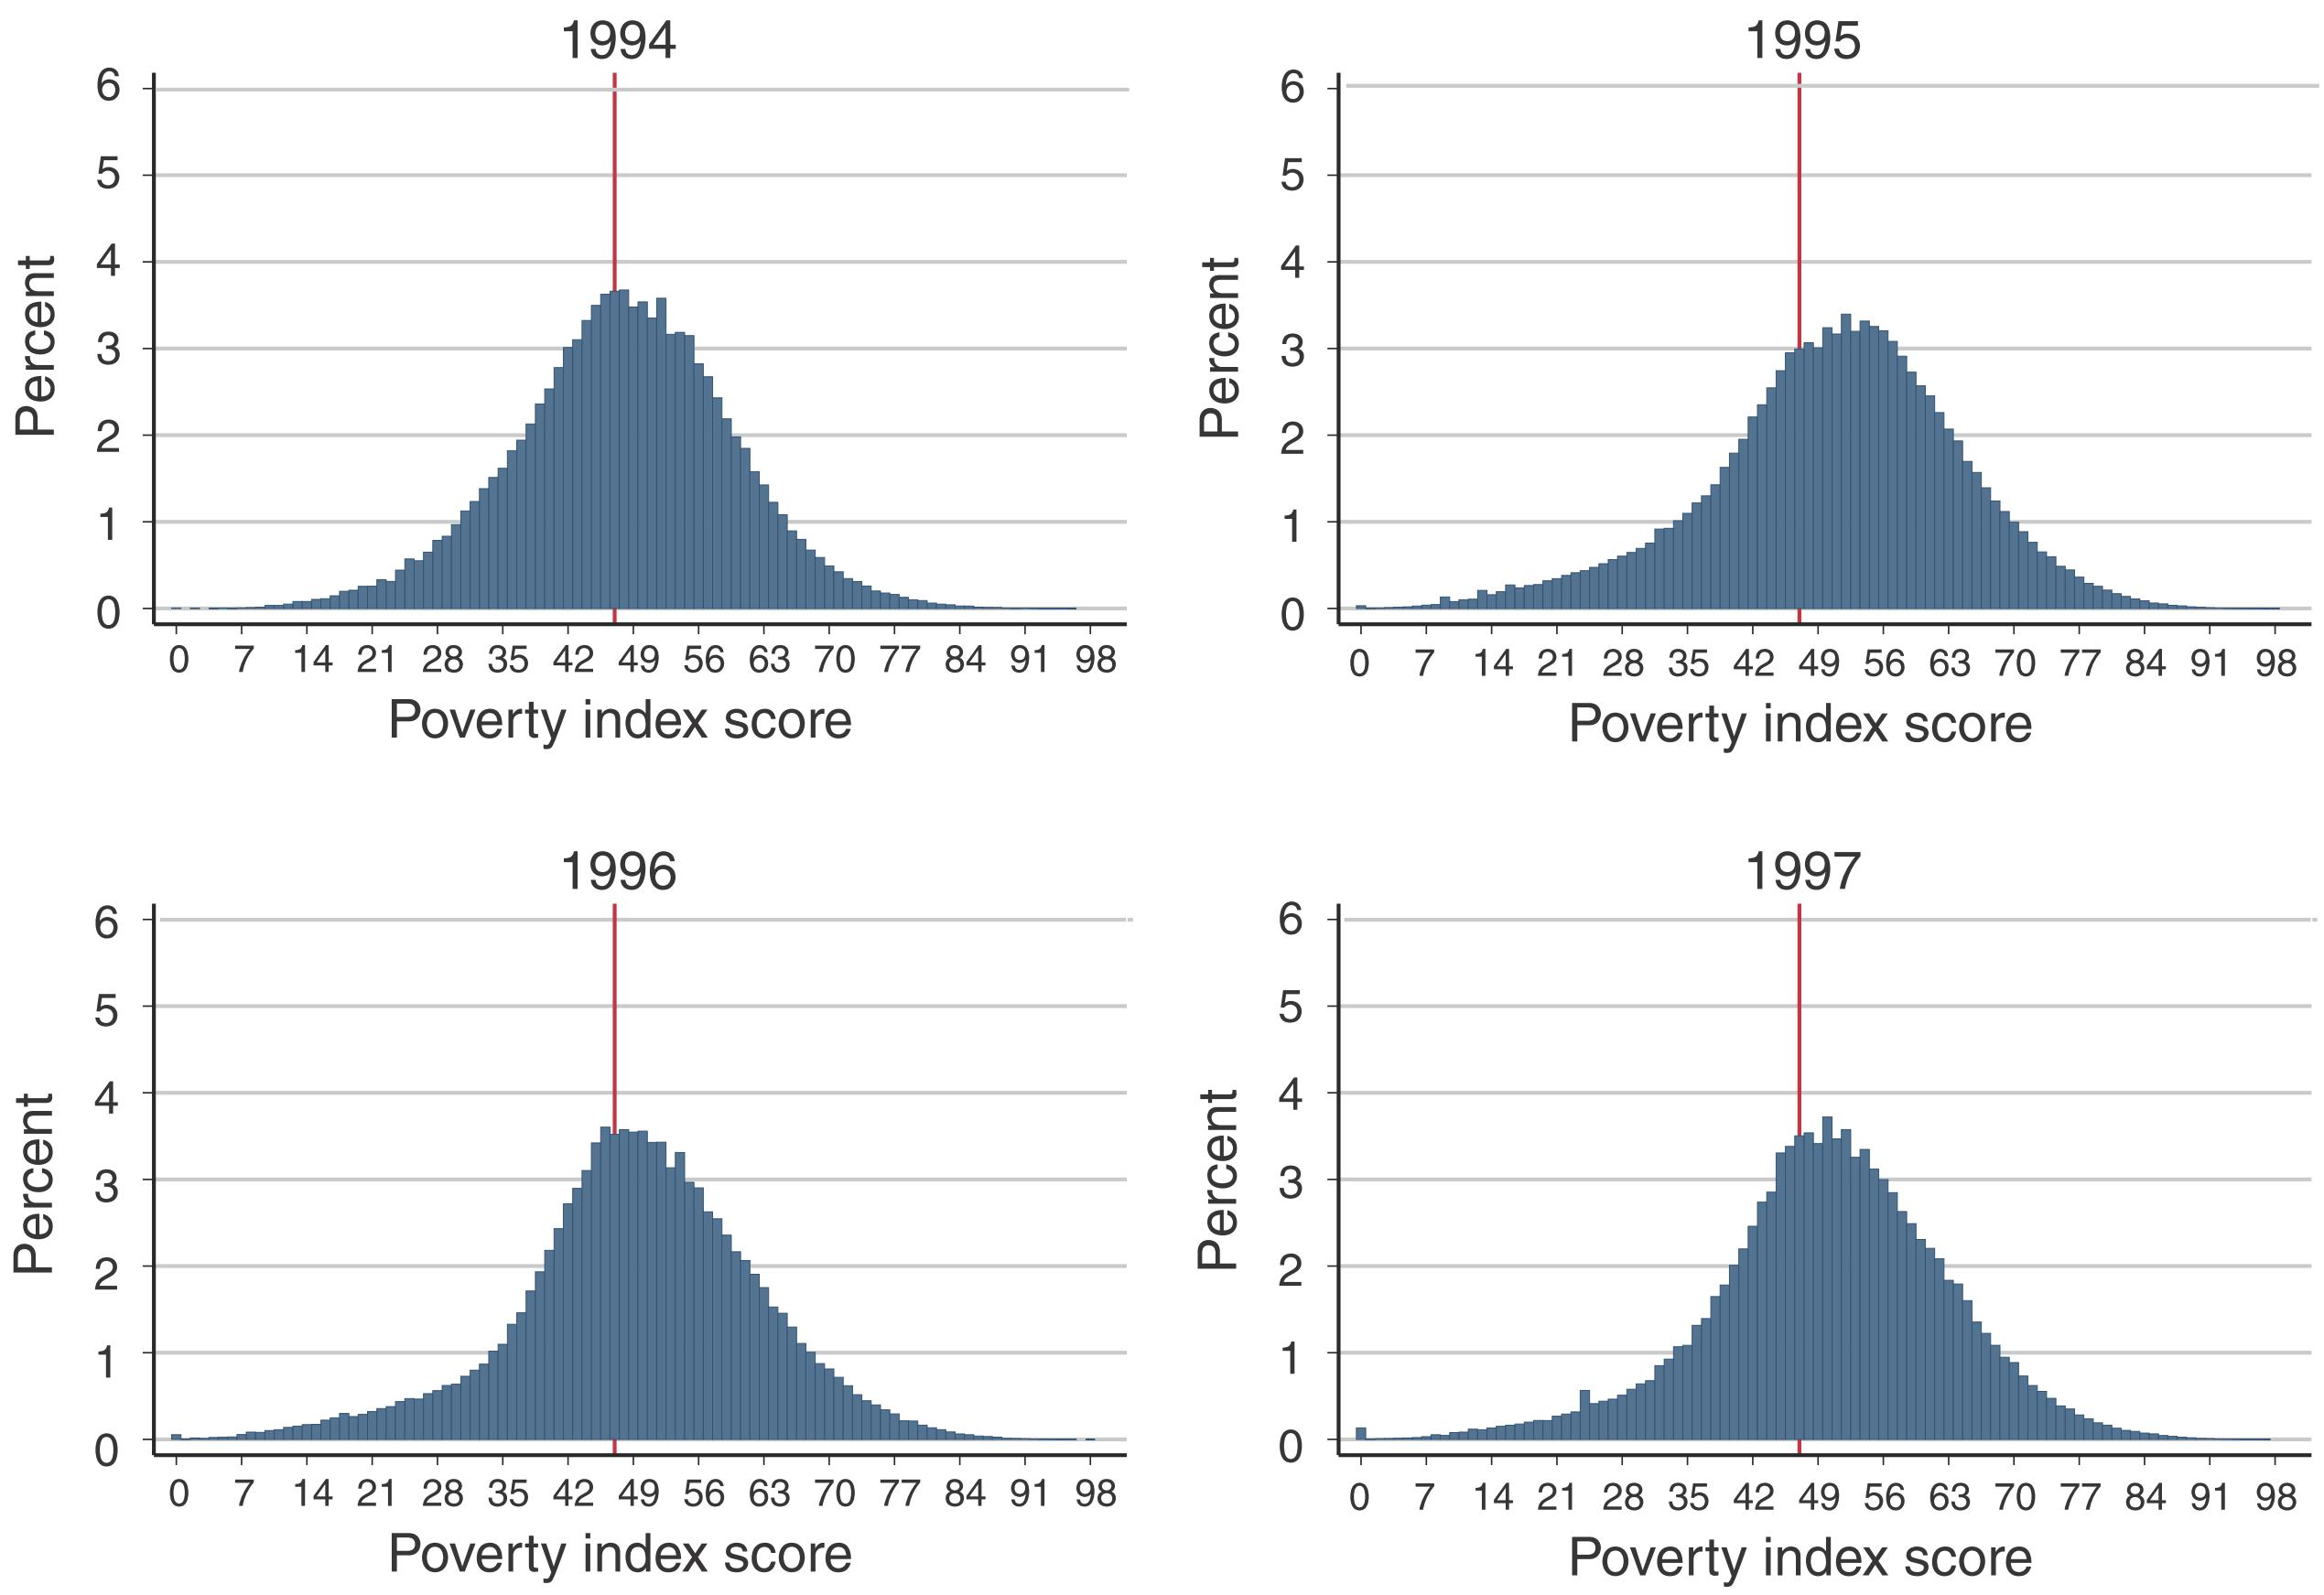
\includegraphics[width=0.9\textwidth]{figure/RD_density_f1.jpg}
	
	
\end{frame}



\begin{frame}{Sorting Behavior}{Example}
	
	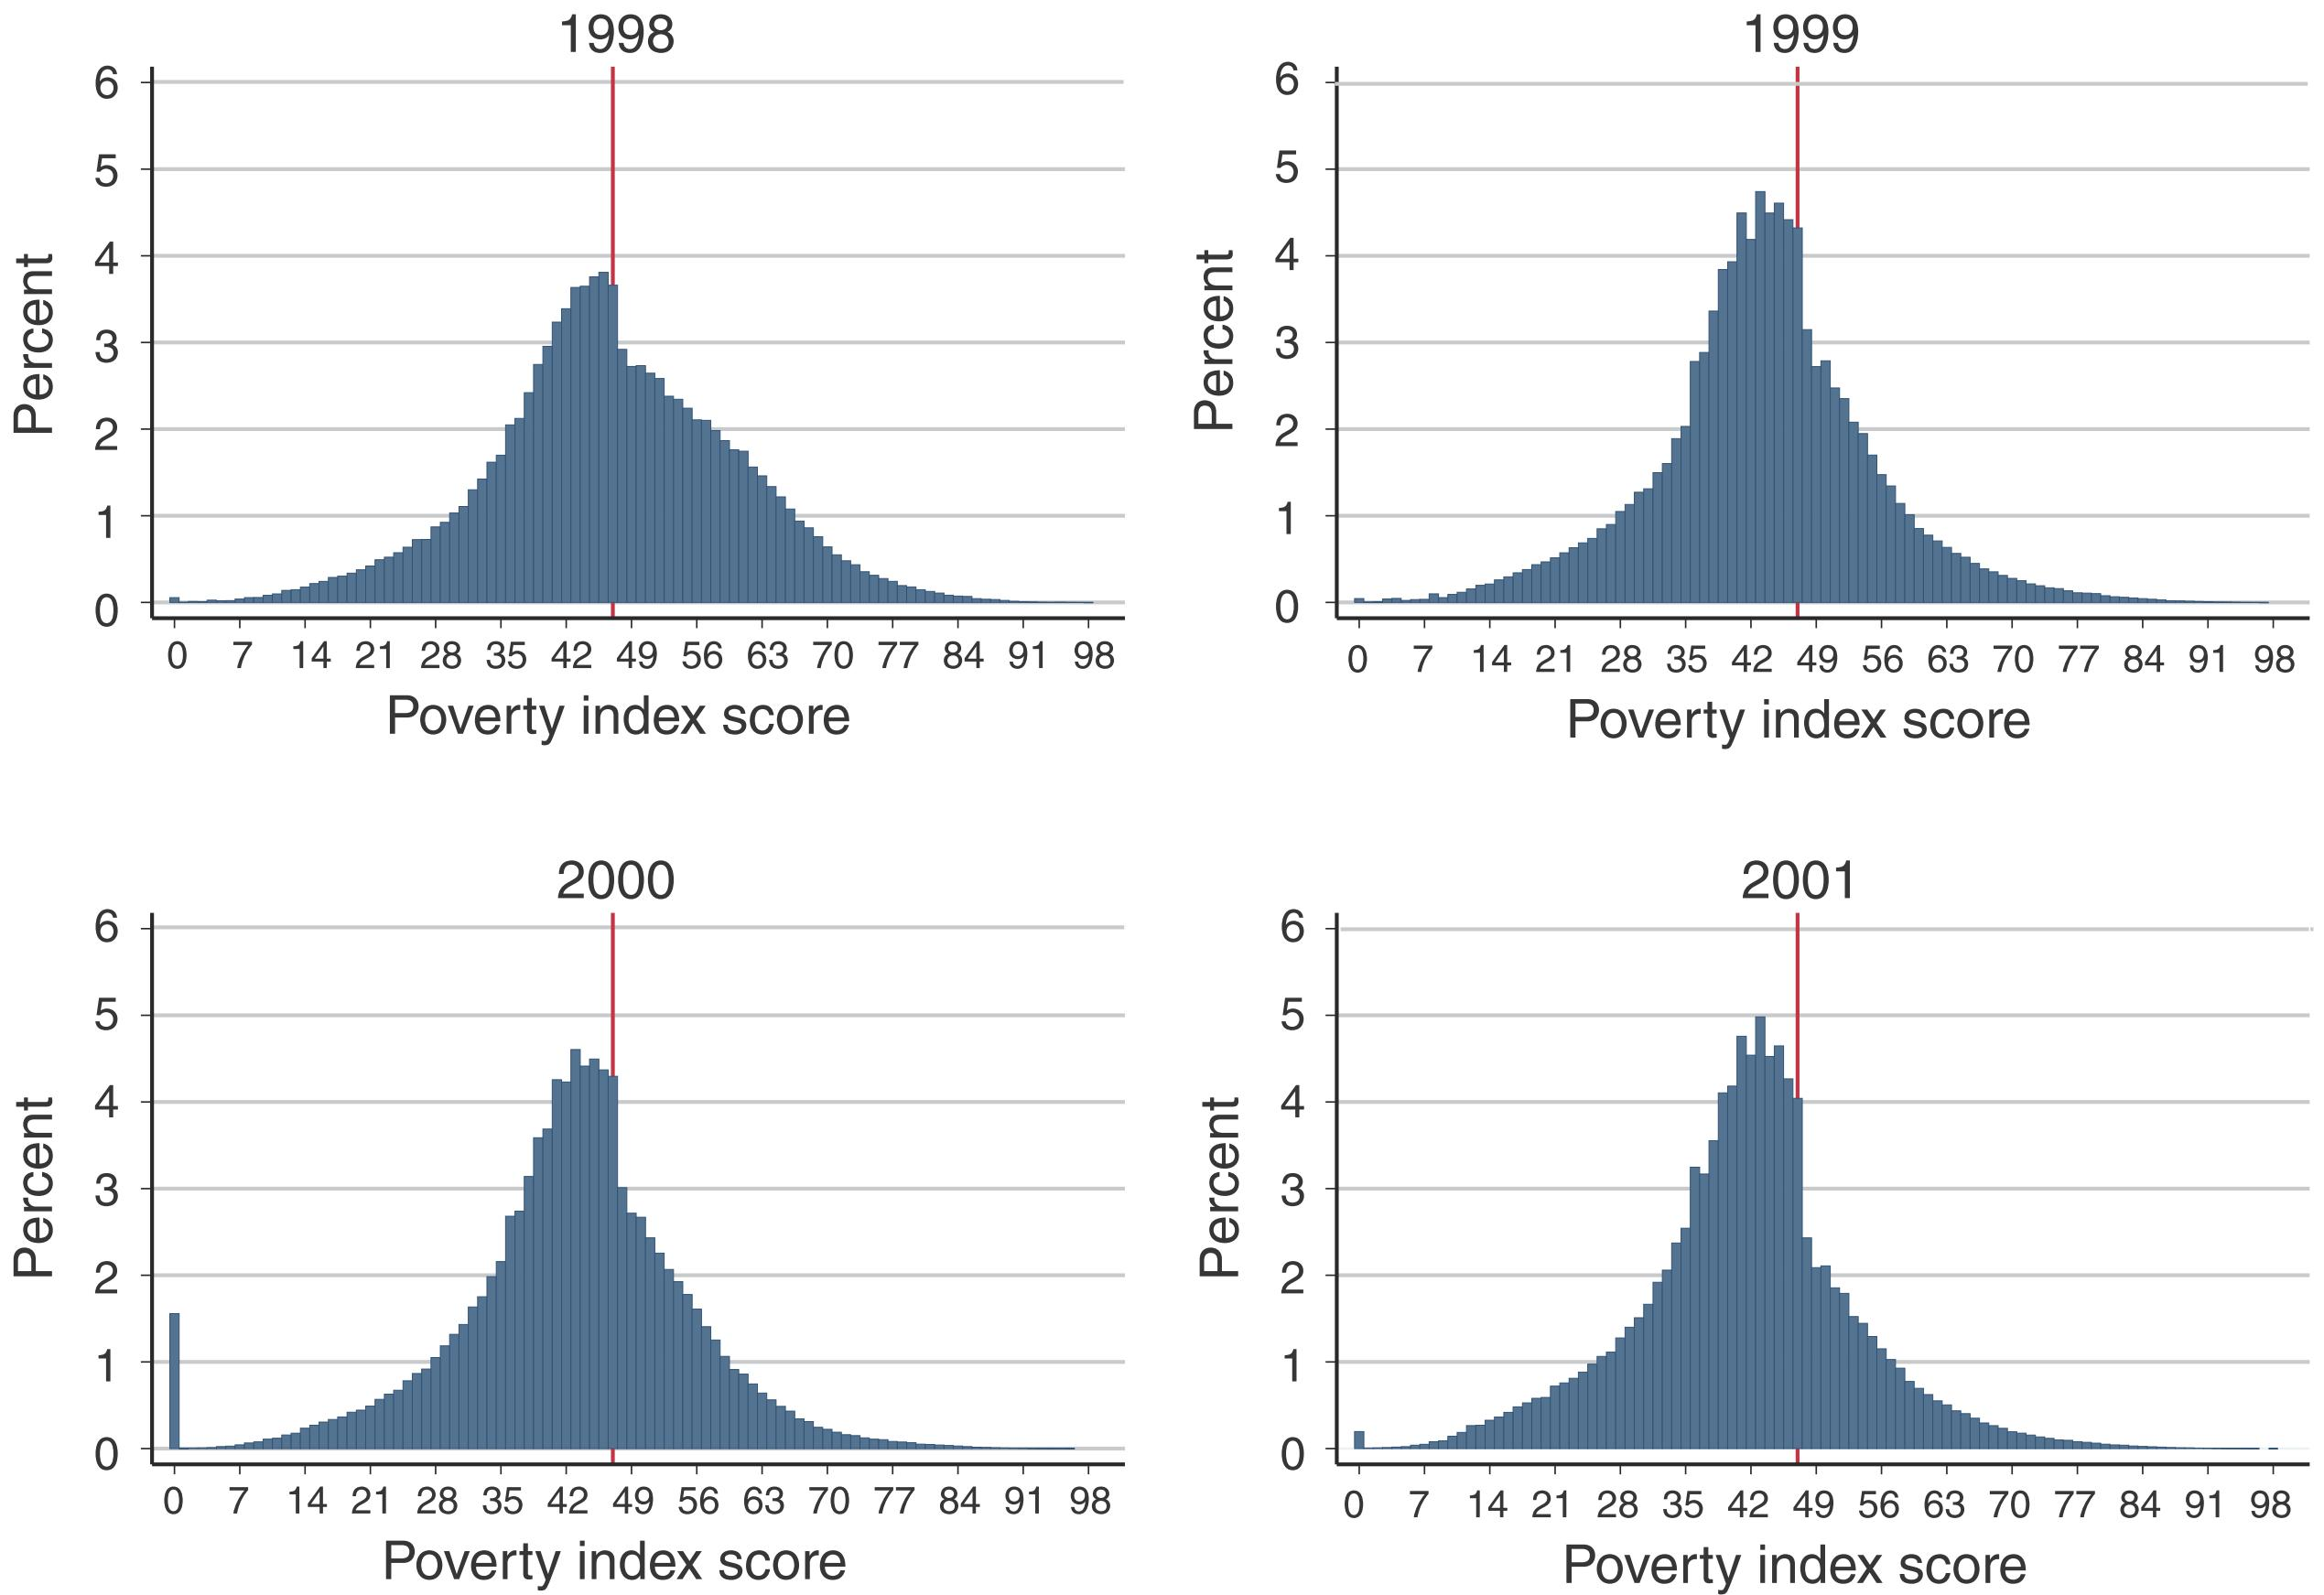
\includegraphics[width=0.9\textwidth]{figure/RD_density_f2.jpg}
	
	
\end{frame}



\begin{frame}{Test Internal Validity of RDD}{Examine Discontinuity in Density of the Assignment Variable}
	
	\textbf{How to Examine ``Discontinuity" in Density of the assignment variable}
	
	\begin{itemize}
		\vspace{0.2cm}	
		\item Plot the number of observations in each bin of assignment variable
		\vspace{0.1cm}	
		\item Investigate whether there is a \textbf{discontinuity in the distribution of the assignment variable} at the threshold
		\vspace{0.2cm}	
			\begin{itemize}
		\item A discontinuity in the density suggests that people might manipulate the assignment variable around the threshold
			\end{itemize}
		
	\end{itemize}
\end{frame}







%\begin{frame}{Test Internal Validity of RDD}{Formal Test for Density Discontinuity (McCrary Test)} % More specific title
%	
%	\begin{itemize}
%		\item A formal statistical test for discontinuity in the density of the assignment variable was proposed by \textbf{McCrary (2008, Journal of Econometrics)}.
%		\vspace{0.3cm}
%		\item \textbf{Key Steps of the McCrary Test}:
%		\vspace{0.1cm}
%		\begin{itemize}
%			\item[1.] \textbf{Binning}: Partition the assignment variable ($A$) into discrete bins. Calculate the number of observations (frequency, $N_j$) for each bin $j$.
%			\vspace{0.2cm}
%			\item[2.] \textbf{Centering}: Ensure that no bin straddles or overlaps the cutoff point $c$. The running variable for the local regressions will be the midpoint of each bin ($x_j$).
%			\vspace{0.2cm}
%			\item[3.] \textbf{Local Linear Regressions}: Run local linear regressions using the bin frequencies ($N_j$) as the outcome variable and bin midpoints ($x_j$) as the covariate. This is done separately for data to the left and to the right of the cutoff $c$.
%			% Y_bin = N_j (frequency counts)
%			% X_bin = x_j (bin midpoints)
%			\vspace{0.2cm}
%			\item[4.] \textbf{Test Statistic ($\theta$)}: The test statistic is the estimated log difference in the heights of the (smoothed) density at the cutoff. This is derived from the difference in the intercepts of the two local linear regressions at $c$.
%			% theta = log(f_R(c)) - log(f_L(c))
%			\vspace{0.2cm}
%			\item[5.] \textbf{Inference}: A statistically significant $\theta \neq 0$ provides evidence of a discontinuity in the density, suggesting potential manipulation of the assignment variable.
%		\end{itemize}
%	\end{itemize}
%\end{frame}









\begin{frame}{Test Internal Validity of RDD}{Examine Density of the assignment variable}
	
	%\textbf{2. Examine ``Discontinuity" in Density of the assignment variable}
	
	\begin{itemize}
		\vspace{0.2cm}	
		\item A formal test is provided by McCrary (2008)
		\vspace{0.2cm}		
		\begin{itemize}
			\item[1] Partition the assignment variable into bins and calculate frequencies (number of observations) in each bins
			\vspace{0.2cm}
			\item[2] Calculate frequencies (number of observations) in each bin	 
			\vspace{0.2cm}
			\item[3] Ensure that no bin overlaps the cutoff
			\vspace{0.2cm}
			\item[4] \textbf{Run two local linear regressions}, one to the right and one to the left of the cutoff
			\vspace{0.2cm}
			\item[5] In these regressions,  the bin midpoints
			are the regressors and \textbf{number of observations is outcome}
			\vspace{0.2cm}
			\item[6] Test whether log difference of the intercepts of the two regressions
			is statistically different from zero	
			
			
		\end{itemize}
		
		%\item A discontinuity in the density suggests that there is some manipulation of R around the threshold going on
		% \vspace{0.2cm}	
		%\item In the first step you partition the assignment variable into bins and calculate frequencies (number of observations) in the bins
		% \vspace{0.2cm}	
		%\item In the second step you treat those frequency counts as dependent variable in a local linear regression as before
		
		
	\end{itemize}
\end{frame}


\begin{frame}{McCrary Test}{}
	
	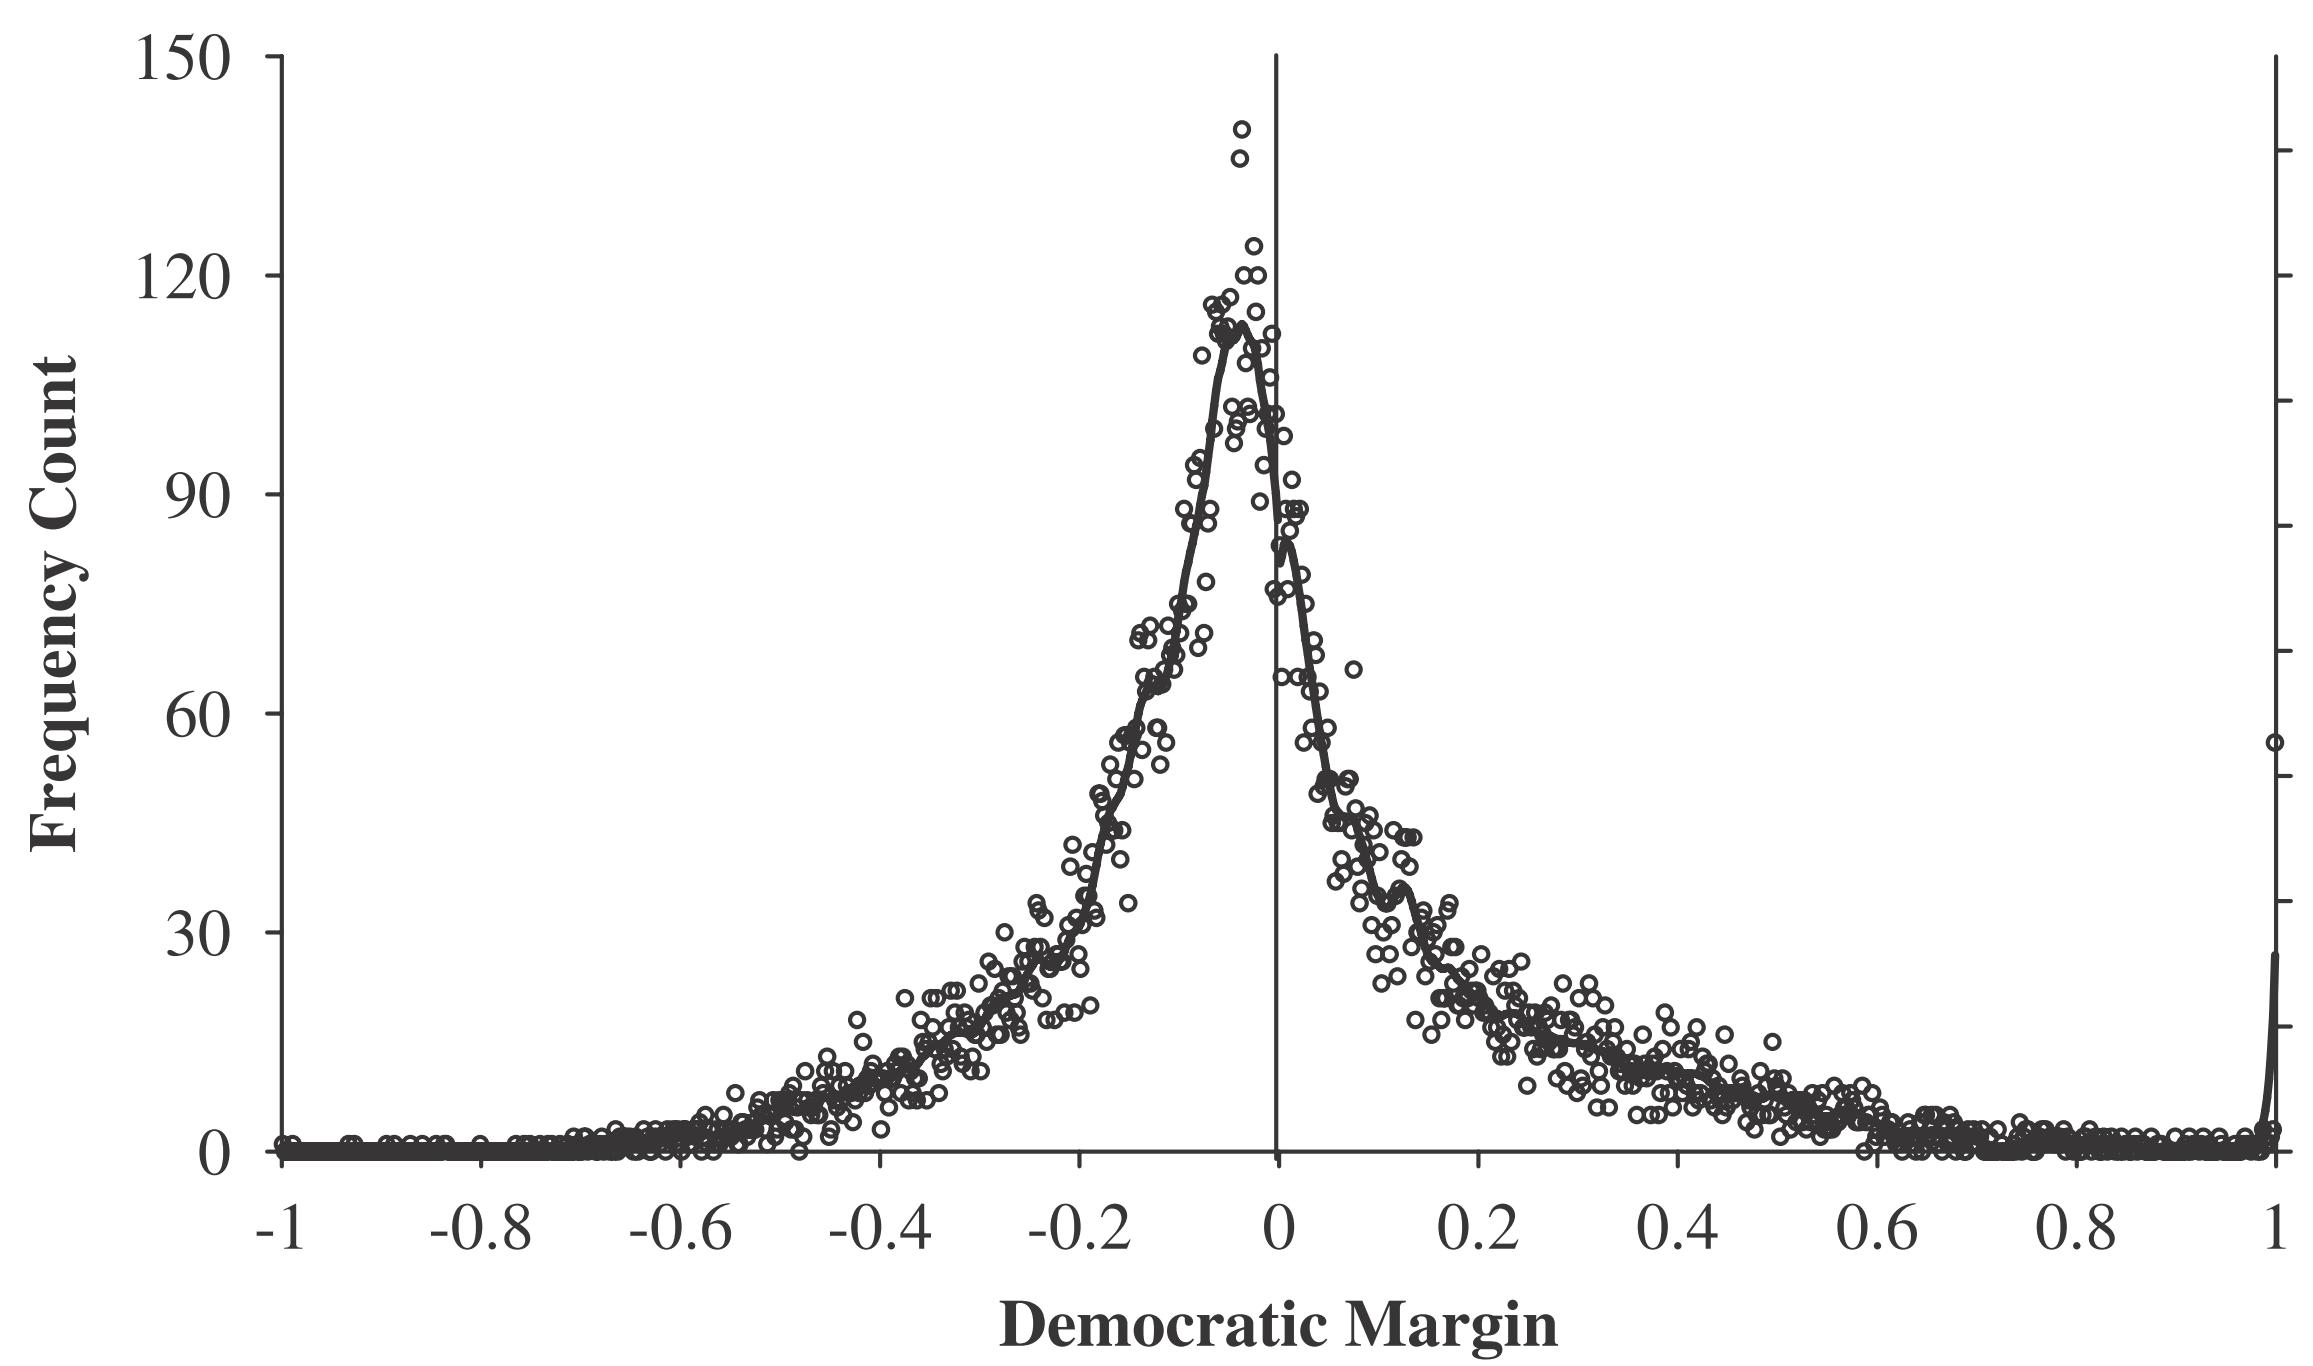
\includegraphics[width=1.0\textwidth]{figure/RD_density_f3.jpg}
	
	
\end{frame}


\begin{frame}{Fuzzy RDD}{Overview}
	\begin{itemize}
		
		\begin{block}{Fuzzy RDD}
			\begin{equation*}
				\lim_{\varepsilon\rightarrow 0}\Pr[D_i=1|A_i=c+\varepsilon] - \lim_{\varepsilon\rightarrow 0}\Pr[D_i=1|A_i=c-\varepsilon] \neq 0
			\end{equation*}
		\end{block}
		
		
		\vspace{0.2cm}
		\item The probability of getting the treatment jumps discontinuously at the cutoff 
		\vspace{0.2cm}
		\begin{itemize}
			\item Some individuals above cutoff do NOT get treatment and some individuals below cutoff do receive treatment
		\end{itemize}
	\end{itemize}
	
	
	%\begin{itemize}		
	%	\item The probability of being admitted to elite university may jump at a certain test score 
	% \vspace{0.2cm}
	%	\item Students still can decide not enroll in that school
	%\end{itemize}
	
	
\end{frame}









\begin{frame}{Treatment Probability and assignment variable}{Fuzzy RDD}
	\begin{figure}
		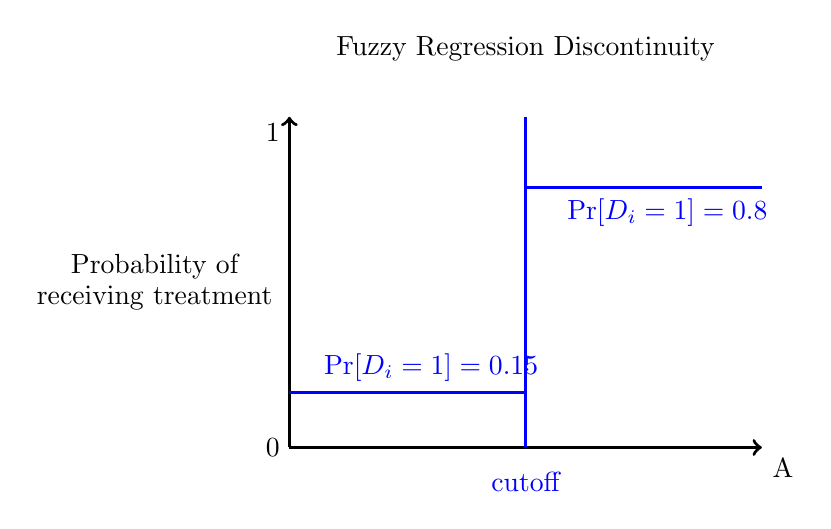
\begin{tikzpicture}[comment/.style={rectangle, text centered}]
			\centering
			\draw[very thick,->] (0,0) -- (6,0) node[anchor=north west] {A};
			\draw[very thick,->] (0,0) -- (0,4.2) node[anchor=south east] {};
			
			\draw[very thick, blue] (3,4.2) -- (3,0) node[anchor=south, yshift=-0.7cm](3_0) {cutoff};
			\draw[very thick, blue] (0,0.7) -- (3,0.7)   node[anchor=south, xshift=-1.2cm] {$\Pr[D_i=1]=0.15$};
			\draw[very thick, blue] (3,3.3) -- (6,3.3)   node[anchor=north, xshift=-1.2cm] {$\Pr[D_i=1]=0.8$};
			
			\draw (0,0) -- (0,0) node[anchor=east](0_0) {$0$};
			\draw (0,4) -- (0,4) node[anchor=east] {$1$};
			
			\node [comment, above of = 3_0, yshift=4.5cm] {Fuzzy Regression Discontinuity};
			\node [comment, left of  = 0_0, yshift=2.3cm, xshift=-0.5cm] {Probability of};
			\node [comment, left of  = 0_0, yshift=1.9cm, xshift=-0.5cm] {receiving treatment};
		\end{tikzpicture}
	\end{figure}
\end{frame}









\title[]  
{Fuzzy RDD: Identification}


\author 
{}

%\institute{Institute of Economics, Academia Sinica  \\ Econ, NTU}
%\institute{Institute of Economics, Academia Sinica  \\ IMES/IDAS, NTU}
\institute{}

%\author 
%{楊子霆 \\ 中研院經濟所}

%\institute 
%{中正大學國際經濟專題研討}




\date
{}


\begin{frame}{}
	\titlepage
\end{frame}






\begin{frame}{Potential Outcomes Framework}
	\begin{itemize}
		
		\item \textcolor{blue}{Treatment Eligibility}
		\begin{align*}
			Z_{i}=\left\lbrace
			\begin{array}{l}
				1\quad \text{if $A_i\geq c$, eligible for a treatment}\\
				0\quad \text{if $A_i< c$, not eligible for a treatment}
			\end{array}\right.
		\end{align*}
		% \begin{itemize}
			%\item $Z_{i}=1$: those who get treatment eligibility (above cutoff)
			% \vspace{0.2cm}
			%\item $Z_{i}=0$: those who do not get treatment eligibility (below cutoff)
			% \vspace{0.2cm}
		% \end{itemize}
		
	\end{itemize}
\end{frame}




\begin{frame}{Potential Outcomes Framework}
	\begin{itemize}
		
		\item \textcolor{blue}{Potential Treatments}
		\vspace{0.2cm}
		\begin{itemize}
			\item $\mathrm{D}^{z}_{i}$: treatment status given the value of $Z$
			\vspace{0.2cm}
			\item $\mathrm{D}^{1}_{i}$: treatment status if eligible for a treatment (above cutoff $c$)
			\vspace{0.2cm}
			
			\begin{align*}
				\mathrm{D}^{1}_{i}=\left\lbrace
				\begin{array}{l}
					1\quad \text{if getting a treatment}\\
					0\quad \text{if not getting a treatment}
				\end{array}\right.
			\end{align*}		
			
			
			\item $\mathrm{D}^{0}_{i}$: treatment status if not eligible for a treatment (below cutoff $c$)
			
			\begin{align*}
				\mathrm{D}^{0}_{i}=\left\lbrace
				\begin{array}{l}
					1\quad \text{if getting a treatment}\\
					0\quad \text{if not getting a treatment}
				\end{array}\right.
			\end{align*}		
			
			
		\end{itemize}
		
	\end{itemize}
\end{frame}






\begin{frame}{Potential Outcomes Framework}
	\begin{itemize}
		
		\item \textcolor{blue}{Observed Treatment}
		\begin{align*}
			D_{i}=\left\lbrace
			\begin{array}{l}
				\mathrm{D}^{1}_{i}\quad \text{if $Z_{i}=1, A_i\geq c$} \\
				\mathrm{D}^{0}_{i}\quad \text{if $Z_{i}=0, A_i< c$}
			\end{array}\right.
		\end{align*}
		\item or, in a more compact notation: 
		$\mathrm{D}_{i}=Z_{i}\mathrm{D}^{1}_{i}+(1-Z_{i})\mathrm{D}^{0}_{i} $
		
	\end{itemize}
\end{frame}



\begin{frame}{Potential Outcomes Framework}
	\begin{itemize}
		
		\item In sharp RDD, the \textbf{eligible for a treatment $Z_{i}$} is the same as \textbf{getting a treatment $D_{i}$} 
		\vspace{0.2cm}
		\begin{itemize}
			\item $Z_{i}=D_{i}$
		\end{itemize}
		
		\vspace{0.2cm}
		\item In fuzzy RDD, the \textbf{eligible for a treatment $Z_{i}$} does NOT represent the \textbf{getting a treatment $D_{i}$} 
		
		\vspace{0.2cm}
		\begin{itemize}
			\item $Z_{i}\neq D_{i}$
		\end{itemize}
		
		
		
		
		
	\end{itemize}
\end{frame}



%\begin{frame}{Potential Outcomes Framework}
%	\begin{itemize}
%		\item The variation in getting a treatment $D_{i}$ (enroll in NTU) was not entirely from the treatment eligibility $Z_{i}$ (passing test score cutoff) but also from individual choice
%		\vspace{0.2cm}
%		\item Thus, $\mathrm{D}^{1}_{i} = 1$ or $\mathrm{D}^{1}_{i}=0$
%		\vspace{0.2cm}
%		\begin{itemize}
%			\item Students whose test score is above threshold can enroll in NTU or not enroll in NTU
%		\end{itemize}
%		\vspace{0.2cm}
%		\item Similarly, $\mathrm{D}^{0}_{i} = 1$ or $\mathrm{D}^{0}_{i}=0$
%		\vspace{0.2cm}
%		\begin{itemize}
%			\item Students whose test score is below threshold can enroll in NTU or not enroll in NTU
%		\end{itemize}
%		
%	\end{itemize}
%\end{frame}









\begin{frame}{Use Passing Cutoff as an IV}{}
	\begin{itemize}
		
		\item The discontinuity in outcome is actually the \textbf{average causal effect} of \textbf{treatment eligibility} $Z_{i}=1(A_i\geq c)$ at cutoff $c$
		
		\begin{equation}
			\lim_{\varepsilon\rightarrow 0}\mathrm{E}[Y_{i}|A_{i}=c+\varepsilon]-\lim_{\varepsilon\rightarrow 0}\mathrm{E}[Y_{i}|A_{i}=c-\varepsilon]	
		\end{equation}
		
		
		\item To recover the causal effect of \textbf{receiving treatment} $D_{i}$
		\vspace{0.2cm}
		\item Divide (2) by the jump in the treatment probability at cutoff
		
		\begin{equation*}
			\lim_{\varepsilon\rightarrow 0}\mathrm{E}[D_{i}|A_{i}=c+\varepsilon]-\lim_{\varepsilon\rightarrow 0}\mathrm{E}[D_{i}|A_{i}=c-\varepsilon]
		\end{equation*}
		
	\end{itemize}
\end{frame}




\begin{frame}{Fuzzy RDD is IV}{}
	\begin{itemize}
		
		\item The the average causal effect of \textbf{receiving treatment} defined in fuzzy RDD :
		
		\begin{equation*}
			\begin{aligned}
				\alpha_{FRD} &=\dfrac{\lim_{\varepsilon\rightarrow 0}\mathrm{E}[Y_{i}|A_{i}=c+\varepsilon]-\lim_{\varepsilon\rightarrow 0}\mathrm{E}[Y_{i}|A_{i}=c-\varepsilon]}{	\lim_{\varepsilon\rightarrow 0}\mathrm{E}[D_{i}|A_{i}=c+\varepsilon]-\lim_{\varepsilon\rightarrow 0}\mathrm{E}[D_{i}|A_{i}=c-\varepsilon]} 
			\end{aligned}
		\end{equation*} 
		
		
		\item This is a \textbf{Wald estimate} at cutoff $c$
		\vspace{0.2cm}
		\item So we can consider fuzzy RDD as an IV estimate
		\vspace{0.2cm}
		\item Use treatment eligibility $Z_{i}=1(A_i\geq c)$ as an instrument for treatment received $D_{i}$
		\vspace{0.2cm}
		\begin{itemize}
			\item Use an indicator for the test score above threshold as an instrument for attending NTU
		\end{itemize}	
	\end{itemize}
\end{frame}





\begin{frame}{Fuzzy RDD is IV}{Assumptions}
	\begin{itemize}
		
		\item \textbf{First-Stage Relationship}: $Z_{i}=1(A_i\geq c)$ affects treatment probability
		
		\vspace{0.2cm}
		\item \textbf{Local Independent Assumption}: In a neighborhood of cutoff $c$
		
		\begin{equation*}
			(\mathrm{Y}^{1}_{i},\mathrm{Y}^{0}_{i}, \mathrm{D}^{1}_{i},\mathrm{D}^{0}_{i})\indep Z_{i}
		\end{equation*}
		\vspace{0.2cm}
		\begin{itemize}
			\item In a neighborhood of cutoff $c$, the assignment to treatment is random		
		\end{itemize}		
		
	\end{itemize}
\end{frame}



\begin{frame}{Fuzzy RDD is IV}{Assumptions}
	\begin{itemize}
		
		
		\item \textbf{Exclusion Restriction}: $Z_{i}=1(A_i\geq c)$ affects outcome $Y_{i}$ only through changing treatment status $D_{i}$
		\vspace{0.2cm}
		\item \textbf{Monotonicity Assumption}: $\mathrm{D}^{1}_{i} \geq \mathrm{D}^{0}_{i}$
		\vspace{0.2cm}
		\begin{itemize}
			\item No one is discouraged from taking the treatment by crossing
			the threshold
		\end{itemize}
		
		
	\end{itemize}
\end{frame}






\begin{frame}{Fuzzy RDD and Compliers}
	\begin{itemize}
		
		\item We can define four types of individuals based on whether they fellow the treatment assignment:
		\vspace{0.2cm}
		\begin{itemize}
			\vspace{0.3cm}
			\item \textbf{Compliers}: $\mathrm{D}^{1}_{i}>\mathrm{D}^{0}_{i}$ ($\mathrm{D}^{0}_{i}=0$ and $\mathrm{D}^{1}_{i}=1$)
			\begin{itemize}
				\item David's test score is above NTU cutoff and enrolled in NTU 
				\vspace{0.2cm}
				\item David's test score is below NTU cutoff and did not enroll in NTU 
			\end{itemize}
			\item \textbf{Always-takers}: $\mathrm{D}^{1}_{i}=\mathrm{D}^{0}_{i}=1$
			\begin{itemize}
				\item John always can enroll in NTU (whether or not his test score is above NTU cutoff)
				\vspace{0.2cm}
			\end{itemize}			
			\item \textbf{Never-takers}: $\mathrm{D}^{1}_{i}=\mathrm{D}^{0}_{i}=0$
			\begin{itemize}
				\item Hank never enroll in NTU (whether or not his test score is above NTU cutoff)
				\vspace{0.2cm}
			\end{itemize}			
			\item \textbf{Defiers}: $\mathrm{D}^{1}_{i}<\mathrm{D}^{0}_{i}$ ($\mathrm{D}^{0}_{i}=1$ and $\mathrm{D}^{1}_{i}=0$)
			\begin{itemize}
				\item Jimmy's test score is above NTU cutoff and did NOT enroll in NTU  
				\vspace{0.2cm}
				\item Jimmy's test score is below NTU cutoff but enrolled in NTU  
			\end{itemize}
			
			
		\end{itemize}
		
	\end{itemize}
\end{frame}




\begin{frame}{Fuzzy RDD and Compliers}{}
	
	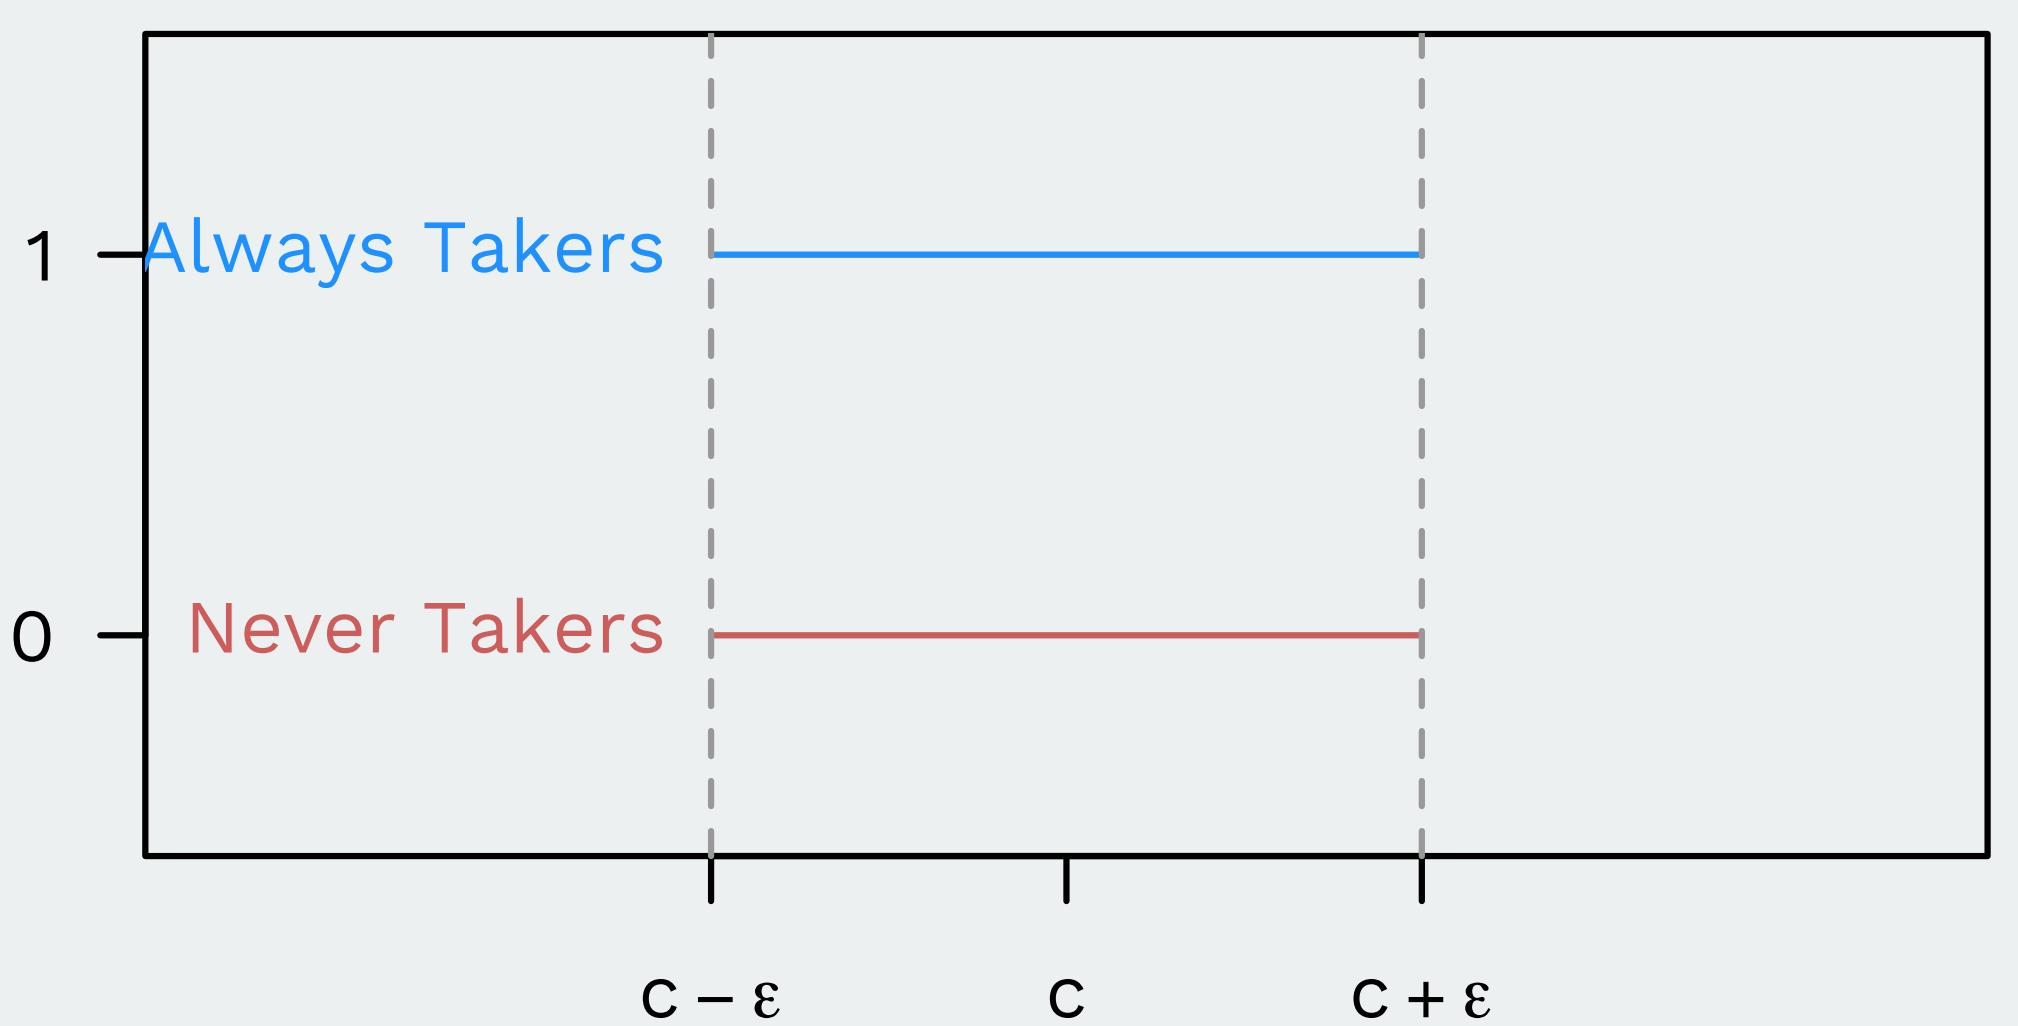
\includegraphics[width=1.0\textwidth]{figure/complier_f1.jpg}
	
	
\end{frame}


\begin{frame}{Fuzzy RDD and Compliers}{}
	
	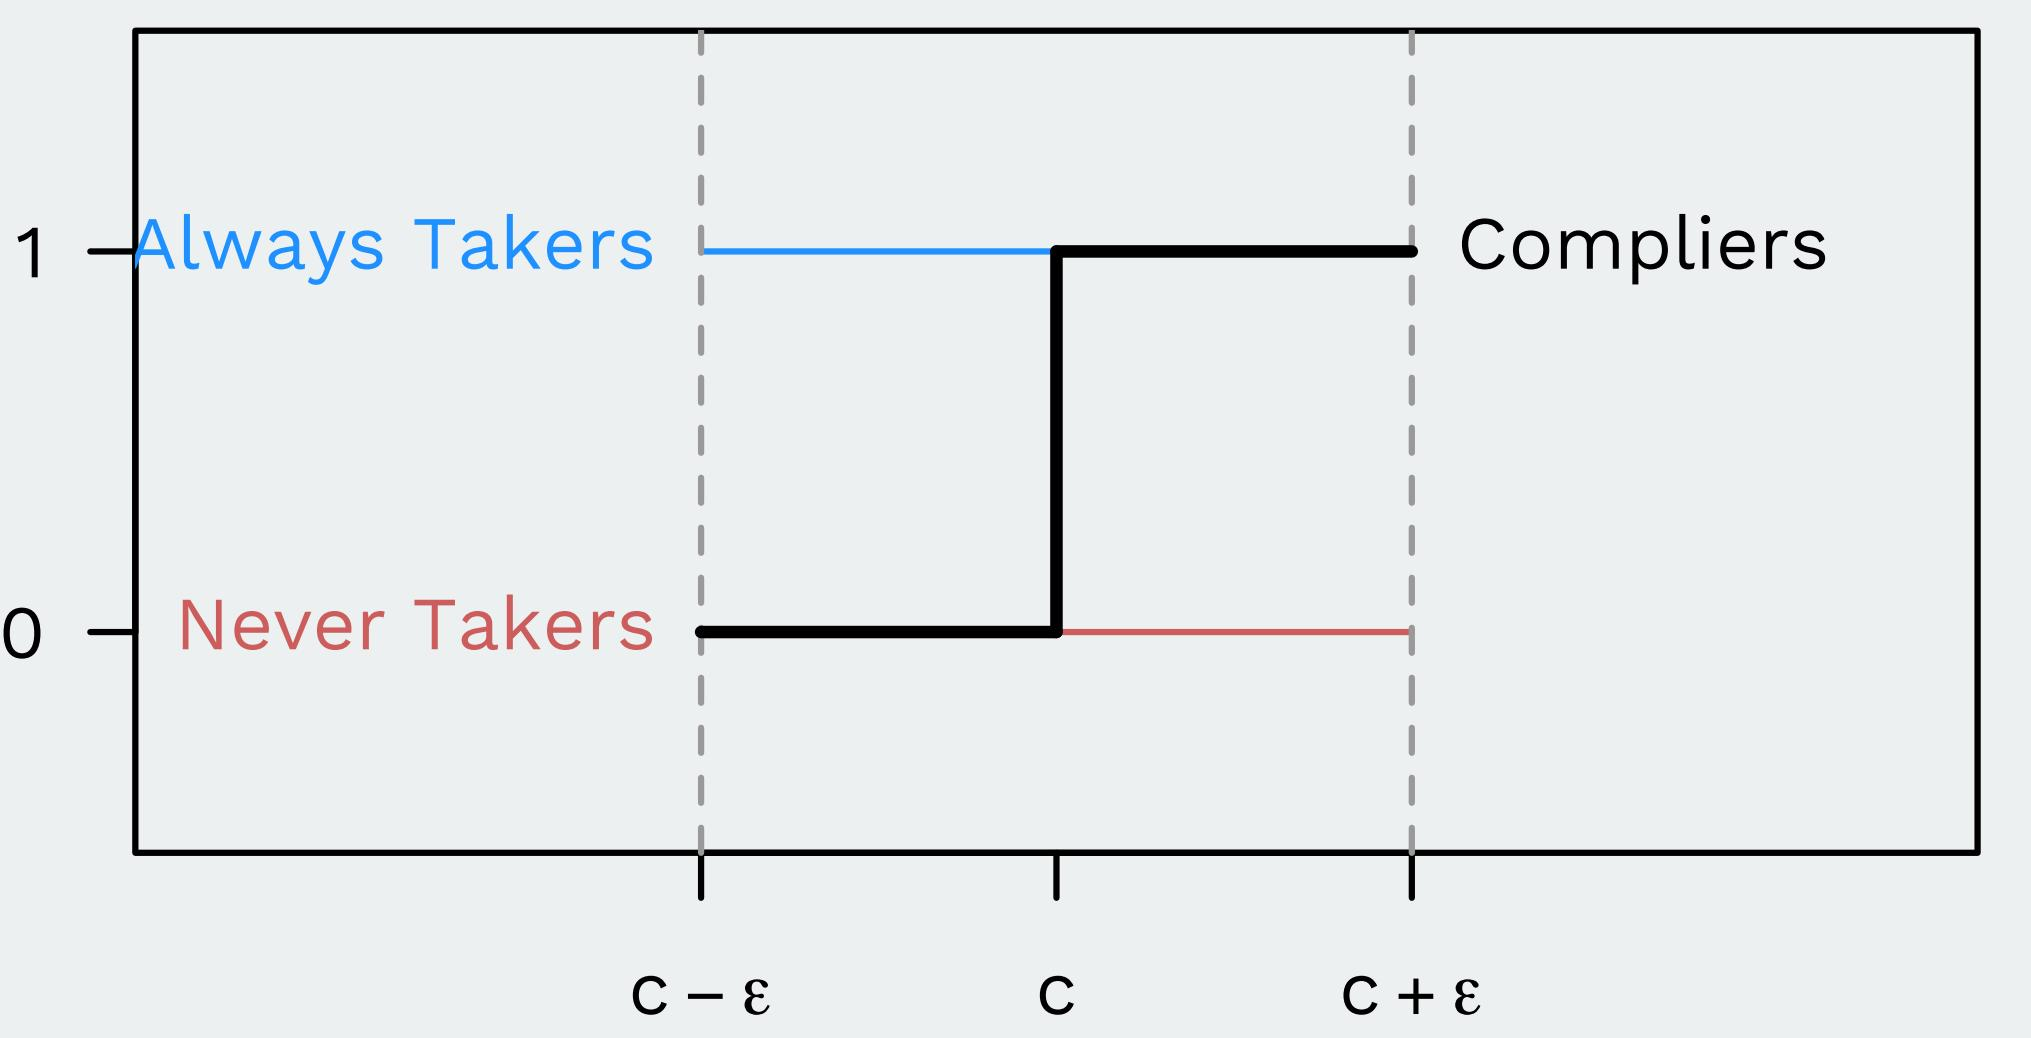
\includegraphics[width=1.0\textwidth]{figure/complier_f2.jpg}
	
	
\end{frame}

\begin{frame}{Identification Results for Fuzzy RDD}
	\begin{itemize}
		
		\begin{block}{Fuzzy RDD Identify LATE at cutoff c}
			\begin{equation*}
				\begin{aligned}
					\alpha_{FRD} &=\dfrac{\lim_{\varepsilon\rightarrow 0}\mathrm{E}[Y_{i}|A_{i}=x+\varepsilon]-\lim_{\varepsilon\rightarrow 0}\mathrm{E}[Y_{i}|A_{i}=x-\varepsilon]}{\lim_{\varepsilon\rightarrow 0}\mathrm{E}[D_{i}|A_{i}=x+\varepsilon]-\lim_{\varepsilon\rightarrow 0}\mathrm{E}[D_{i}|A_{i}=x-\varepsilon]}  \\
					&= \mathrm{E}[ \mathrm{Y}^{1}_{i} - \mathrm{Y}^{0}_{i} | \mathrm{D}^{1}_{i} > \mathrm{D}^{0}_{i}, A_{i}=c]
				\end{aligned}
			\end{equation*} 
		\end{block}
		
		
		\item The estimate in fuzzy RDD represents the \textbf{causal effect for compliers} (local average treatment effect, LATE) at cutoff $c$
		\vspace{0.2cm}
		\item \textbf{Compliers} are those who receive the
		treatment when they follow treatment eligibility rule 
		($A_i\geq c$), but would not otherwise receive it ($A_i< c$)	
		%\item Lottery IV can identify the causal effect of military service on lifetime earnings for those who obey the lottery results (e.g. David and Tim)
	\end{itemize}
\end{frame}






\title[]  
{Fuzzy RDD: Estimation}


\author 
{}

%\institute{Institute of Economics, Academia Sinica  \\ Econ, NTU}
%\institute{Institute of Economics, Academia Sinica  \\ IMES/IDAS, NTU}
\institute{}

%\author 
%{楊子霆 \\ 中研院經濟所}

%\institute 
%{中正大學國際經濟專題研討}




\date
{}


\begin{frame}{}
	\titlepage
\end{frame}






\begin{frame}{Fuzzy RDD}{Estimation}
	\begin{itemize}
		\item Fuzzy RDD implies the discontinuity in treatment assignment $Z_{i}$ can act as an instrument for actual receipt of treatment $D_{i}$
		\vspace{0.2cm}
		\item Therefore, we can estimate treatment effect in fuzzy RDD by using two-stage least squares (TSLS)
		
		\begin{equation*}
			\begin{aligned}
				D_i=\alpha_{1}+\rho_{1} Z_i+\mathrm{f}_{1}(A_i)+\upsilon_i   \\
				Y_i=\alpha_{2}+\rho_{2} D_i+\mathrm{f}_{2}(A_i)+\eta_i
			\end{aligned}
		\end{equation*}
		
		\item As in the sharp RDD setting, we can use either parametric or nonparametric approaches to estimate treatment effect
		
	\end{itemize}
\end{frame}





\title[]  
{Fuzzy RDD: Empirical Example}


\author 
{}

%\institute{Institute of Economics, Academia Sinica  \\ Econ, NTU}
%\institute{Institute of Economics, Academia Sinica  \\ IMES/IDAS, NTU}
\institute{}

%\author 
%{楊子霆 \\ 中研院經濟所}

%\institute 
%{中正大學國際經濟專題研討}




\date
{}


\begin{frame}{}
	\titlepage
\end{frame}


\begin{frame}{Bleemer \& Mehta (2022)}{Motivation}
	
	Zachary Bleemer and Aashish Mehta (2022) ``\textbf{Will Studying Economics Make You Rich? A Regression Discontinuity Analysis of the Returns to College Major}", American Economic Journal: Applied Economics
	
	\begin{itemize}
				\vspace{0.2cm}
		\item Examine the causal effect of majoring in economics on early-career earnings
		
		\vspace{0.2cm}
		\item Key Research Questions:
				\vspace{0.2cm}
		\begin{itemize}
			\item What is the wage return to studying economics?
					\vspace{0.2cm}
			\item How does access to economics major affect students' career paths?
					\vspace{0.2cm}
			\item Do observational wage differences reflect causal effects?
		\end{itemize}
	\end{itemize}
	
\end{frame}

\begin{frame}{Empirical Example: Bleemer \& Mehta (2022)}{Motivation}
	\begin{itemize}
		\item College graduates with economics degrees earn substantially higher wages
		\vspace{0.2cm}
		\begin{itemize}
			\item Median wage of \$90,000 for economics majors vs. \$65,000 for other social sciences
		\end{itemize}
		
		\vspace{0.2cm}
		\item However, estimating causal effects is challenging due to:
					\vspace{0.2cm}
		\begin{itemize}
			\item Students' nonrandom selection into majors
			\vspace{0.2cm}
			\item Universities' admissions and grade requirements
		\end{itemize}
		
		\vspace{0.2cm}
		\item Study exploits a GPA threshold policy at UC Santa Cruz that restricted access to the economics major
		\begin{itemize}
						\vspace{0.2cm}
			\item Students needed 2.8 GPA in Economics 1 \& 2 to declare major
		\end{itemize}
		
	\end{itemize}
\end{frame}


\begin{frame}{Empirical Example: Bleemer \& Mehta (2022)}{Identification Strategy}
	\begin{itemize}
		\item \textbf{Fuzzy RDD}: Exploits GPA threshold (2.8) in Economics 1 and 2 for major access
		
		\vspace{0.2cm}
		\begin{equation*}
			\begin{aligned}
				\alpha_{FRD} &=\dfrac{\lim_{\varepsilon\rightarrow 0}\mathrm{E}[Y_{i}|A_{i}=c+\varepsilon]-\lim_{\varepsilon\rightarrow 0}\mathrm{E}[Y_{i}|A_{i}=c-\varepsilon]}{\lim_{\varepsilon\rightarrow 0}\mathrm{E}[D_{i}|A_{i}=c+\varepsilon]-\lim_{\varepsilon\rightarrow 0}\mathrm{E}[D_{i}|A_{i}=c-\varepsilon]} 
			\end{aligned}
		\end{equation*} 
		
		\item Where:
		\begin{itemize}
					\vspace{0.2cm}
			\item $Y_i$: Early-career wages (2017-2018)
					\vspace{0.2cm}
			\item $A_i$: Average GPA in Economics 1 \& 2
					\vspace{0.2cm}
			\item $D_i$: Economics major indicator
					\vspace{0.2cm}
			\item $c$: GPA threshold (2.8)
		\end{itemize}
	\end{itemize}
\end{frame}




\begin{frame}{Empirical Example: Bleemer \& Mehta (2022)}{Empirical Specification}
	\begin{itemize}
		\item \textbf{First Stage}:
		\begin{equation*}
			D_i = \alpha_1 + \rho_1 Z_i + \mathrm{f}_1(A_i) + \upsilon_i
		\end{equation*}
		
		\item \textbf{Reduced Form}:
		\begin{equation*}
			Y_i = \alpha_2 + \rho_2 Z_i + \mathrm{f}_2(A_i) + \eta_i
		\end{equation*}
		
		\item Where:
		\begin{itemize}
			\item $D_i$: Economics major indicator
			\item $Z_i = 1(A_i \geq 2.8)$: Treatment eligibility
			\item $A_i$: Average GPA in Economics 1 \& 2
			\item $\mathrm{f}_1(.), \mathrm{f}_2(.)$: Linear functions of GPA
		\end{itemize}
		
		\vspace{0.2cm}
		\item \textbf{Fuzzy RD Estimate}:
		\begin{equation*}
			\alpha_{FRD} = \frac{\rho_2}{\rho_1} = \mathrm{E}[ \mathrm{Y}^1_i - \mathrm{Y}^0_i | \mathrm{D}^1_i > \mathrm{D}^0_i, A_i=2.8]
		\end{equation*}
	\end{itemize}
\end{frame}







\begin{frame}{Empirical Example: Bleemer \& Mehta (2022)}{First Stage}
	
	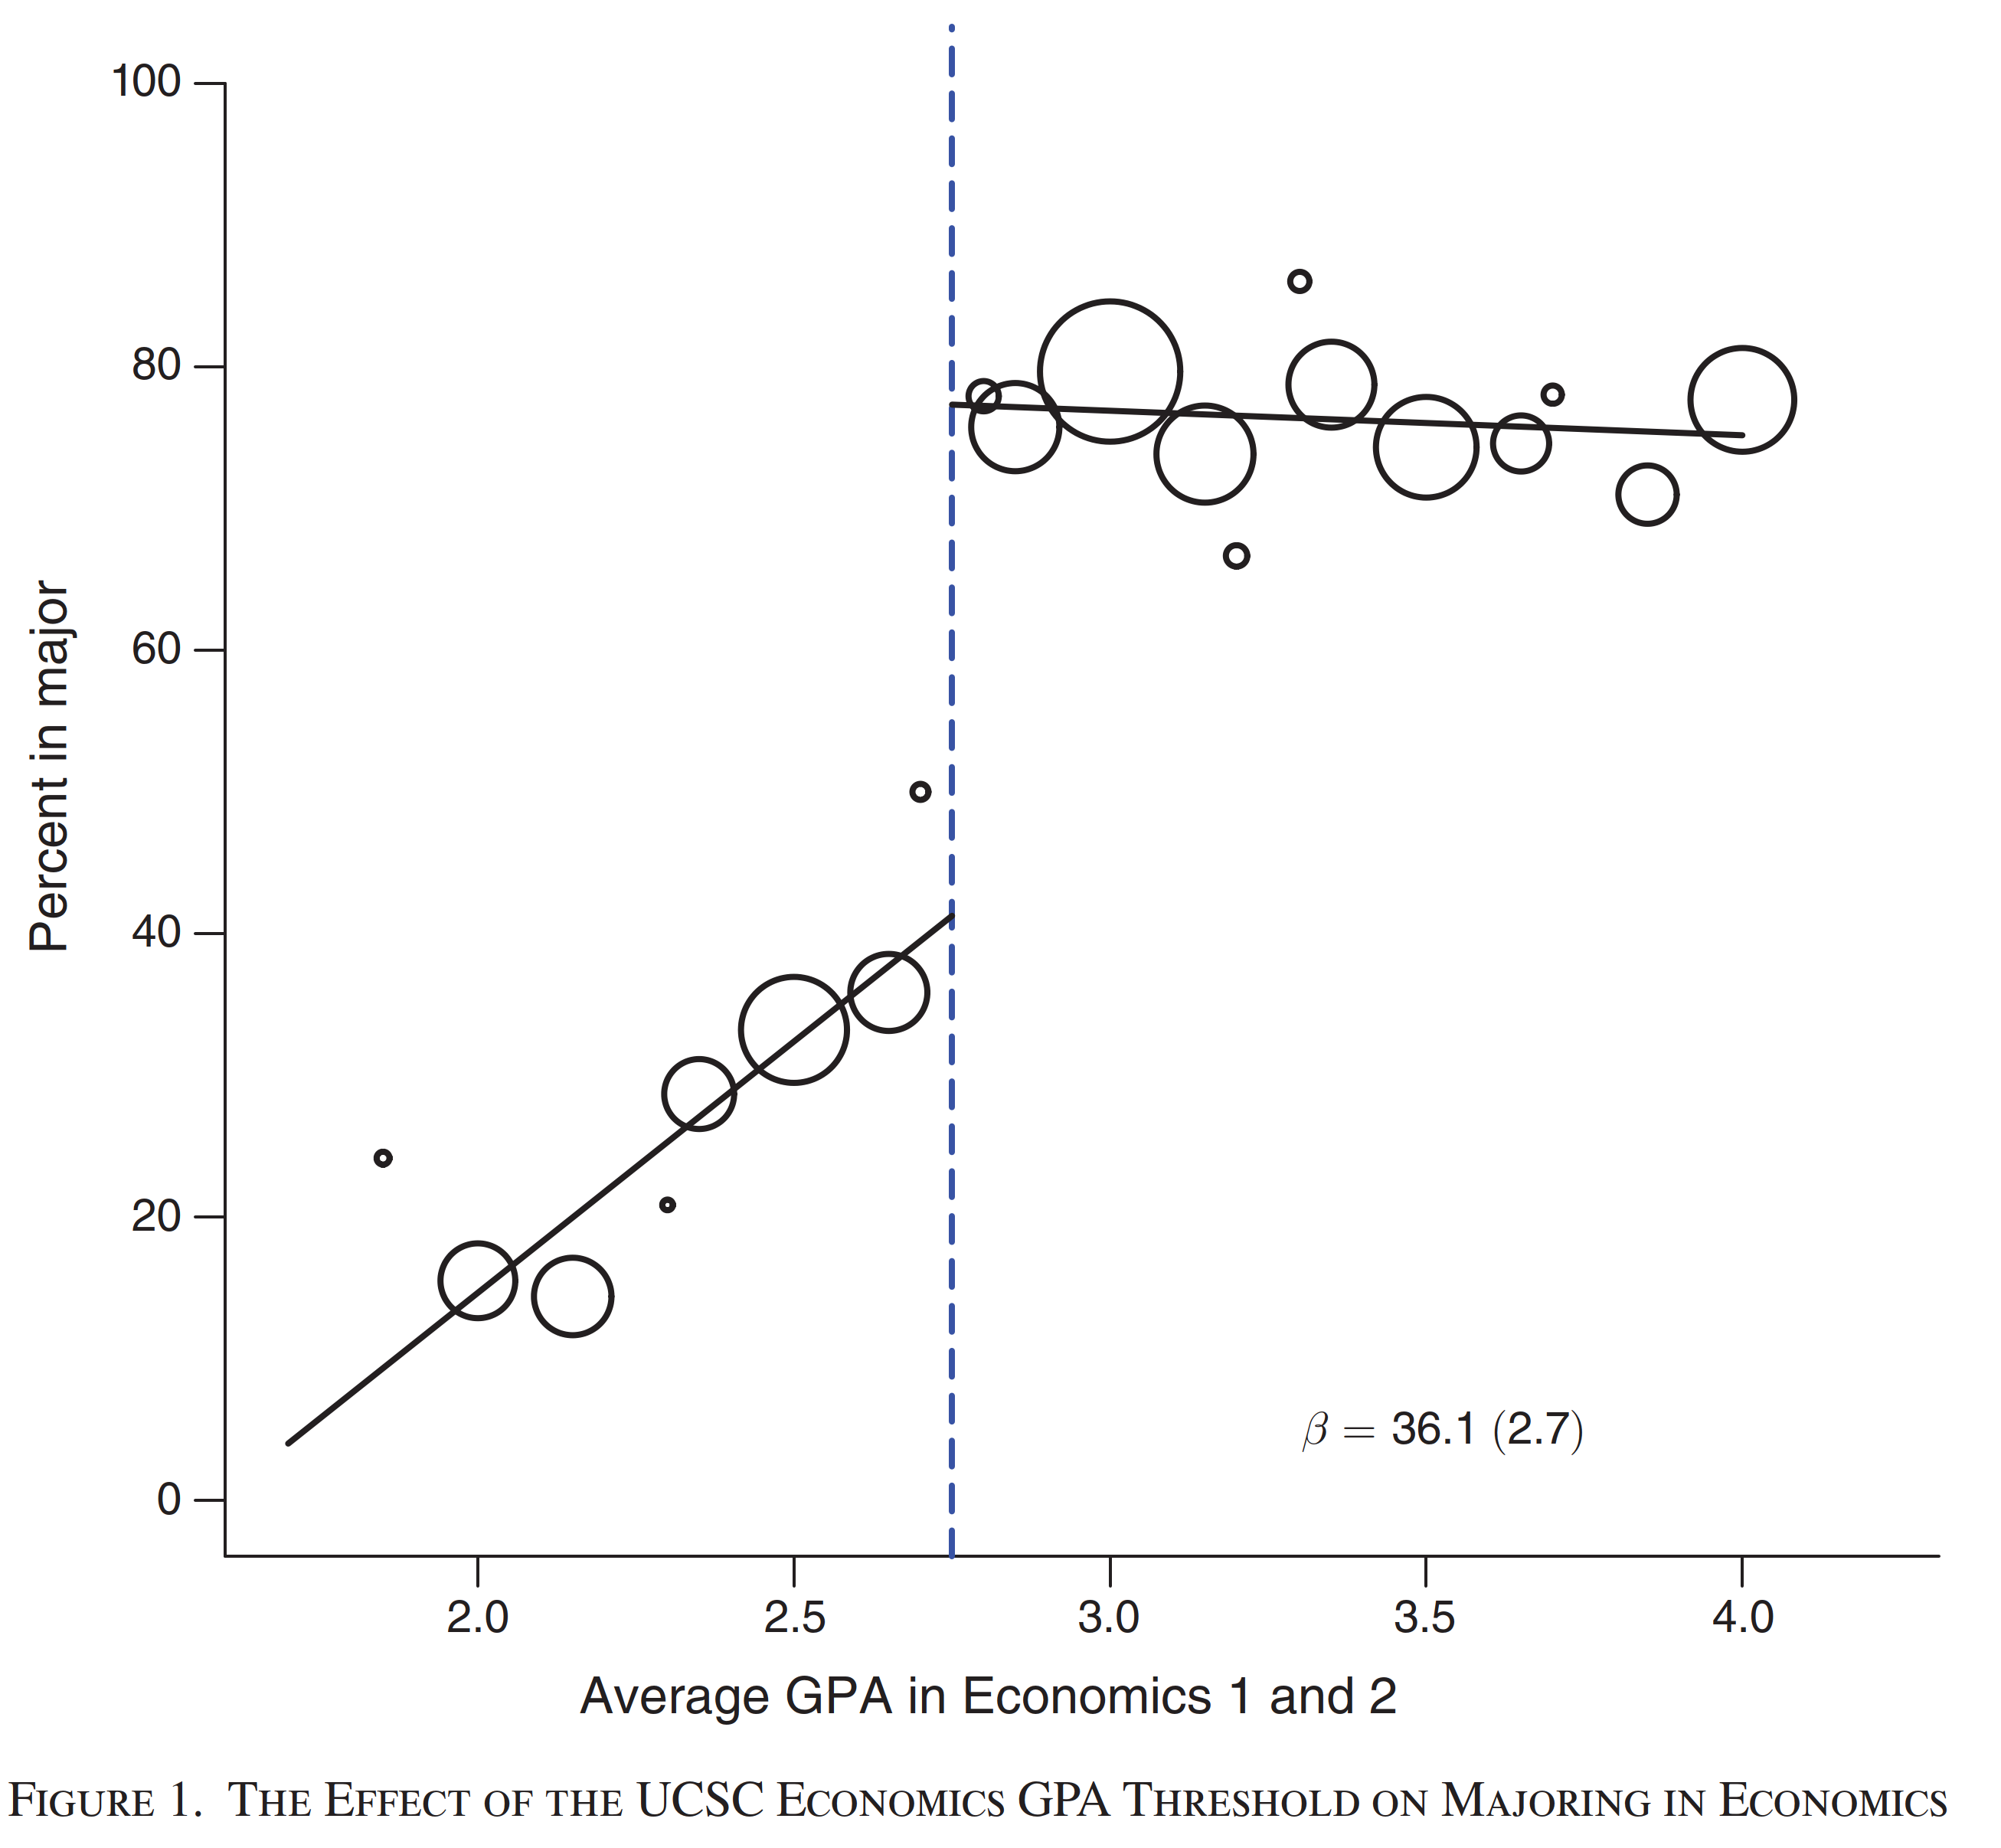
\includegraphics[width=0.60\textwidth]{figure/RD_econ_major_f1.png}
	
	
\end{frame}



\begin{frame}{Empirical Example: Bleemer \& Mehta (2022)}{First Stage}
	\begin{itemize}
		\item Students just above 2.8 GPA threshold were:
		\vspace{0.2cm}
		\begin{itemize}
			\item 36 percentage points more likely to major in economics
			\vspace{0.2cm}
			\item Most would have otherwise majored in other social sciences
			\vspace{0.2cm}
		\end{itemize}
		
		%		\item Compliers are representative of economics majors:
		%				\vspace{0.2cm}
		%		\begin{itemize}
			%			\item 36\% female (vs. 41\% all econ majors)
			%					\vspace{0.2cm}
			%			\item 41\% Asian (vs. 44\% all econ majors)
			%					\vspace{0.2cm}
			%			\item SAT scores at 41st percentile of econ majors
			%		\end{itemize}
	\end{itemize}
\end{frame}



\begin{frame}{Empirical Example: Bleemer \& Mehta (2022)}{Second Stage}
	
	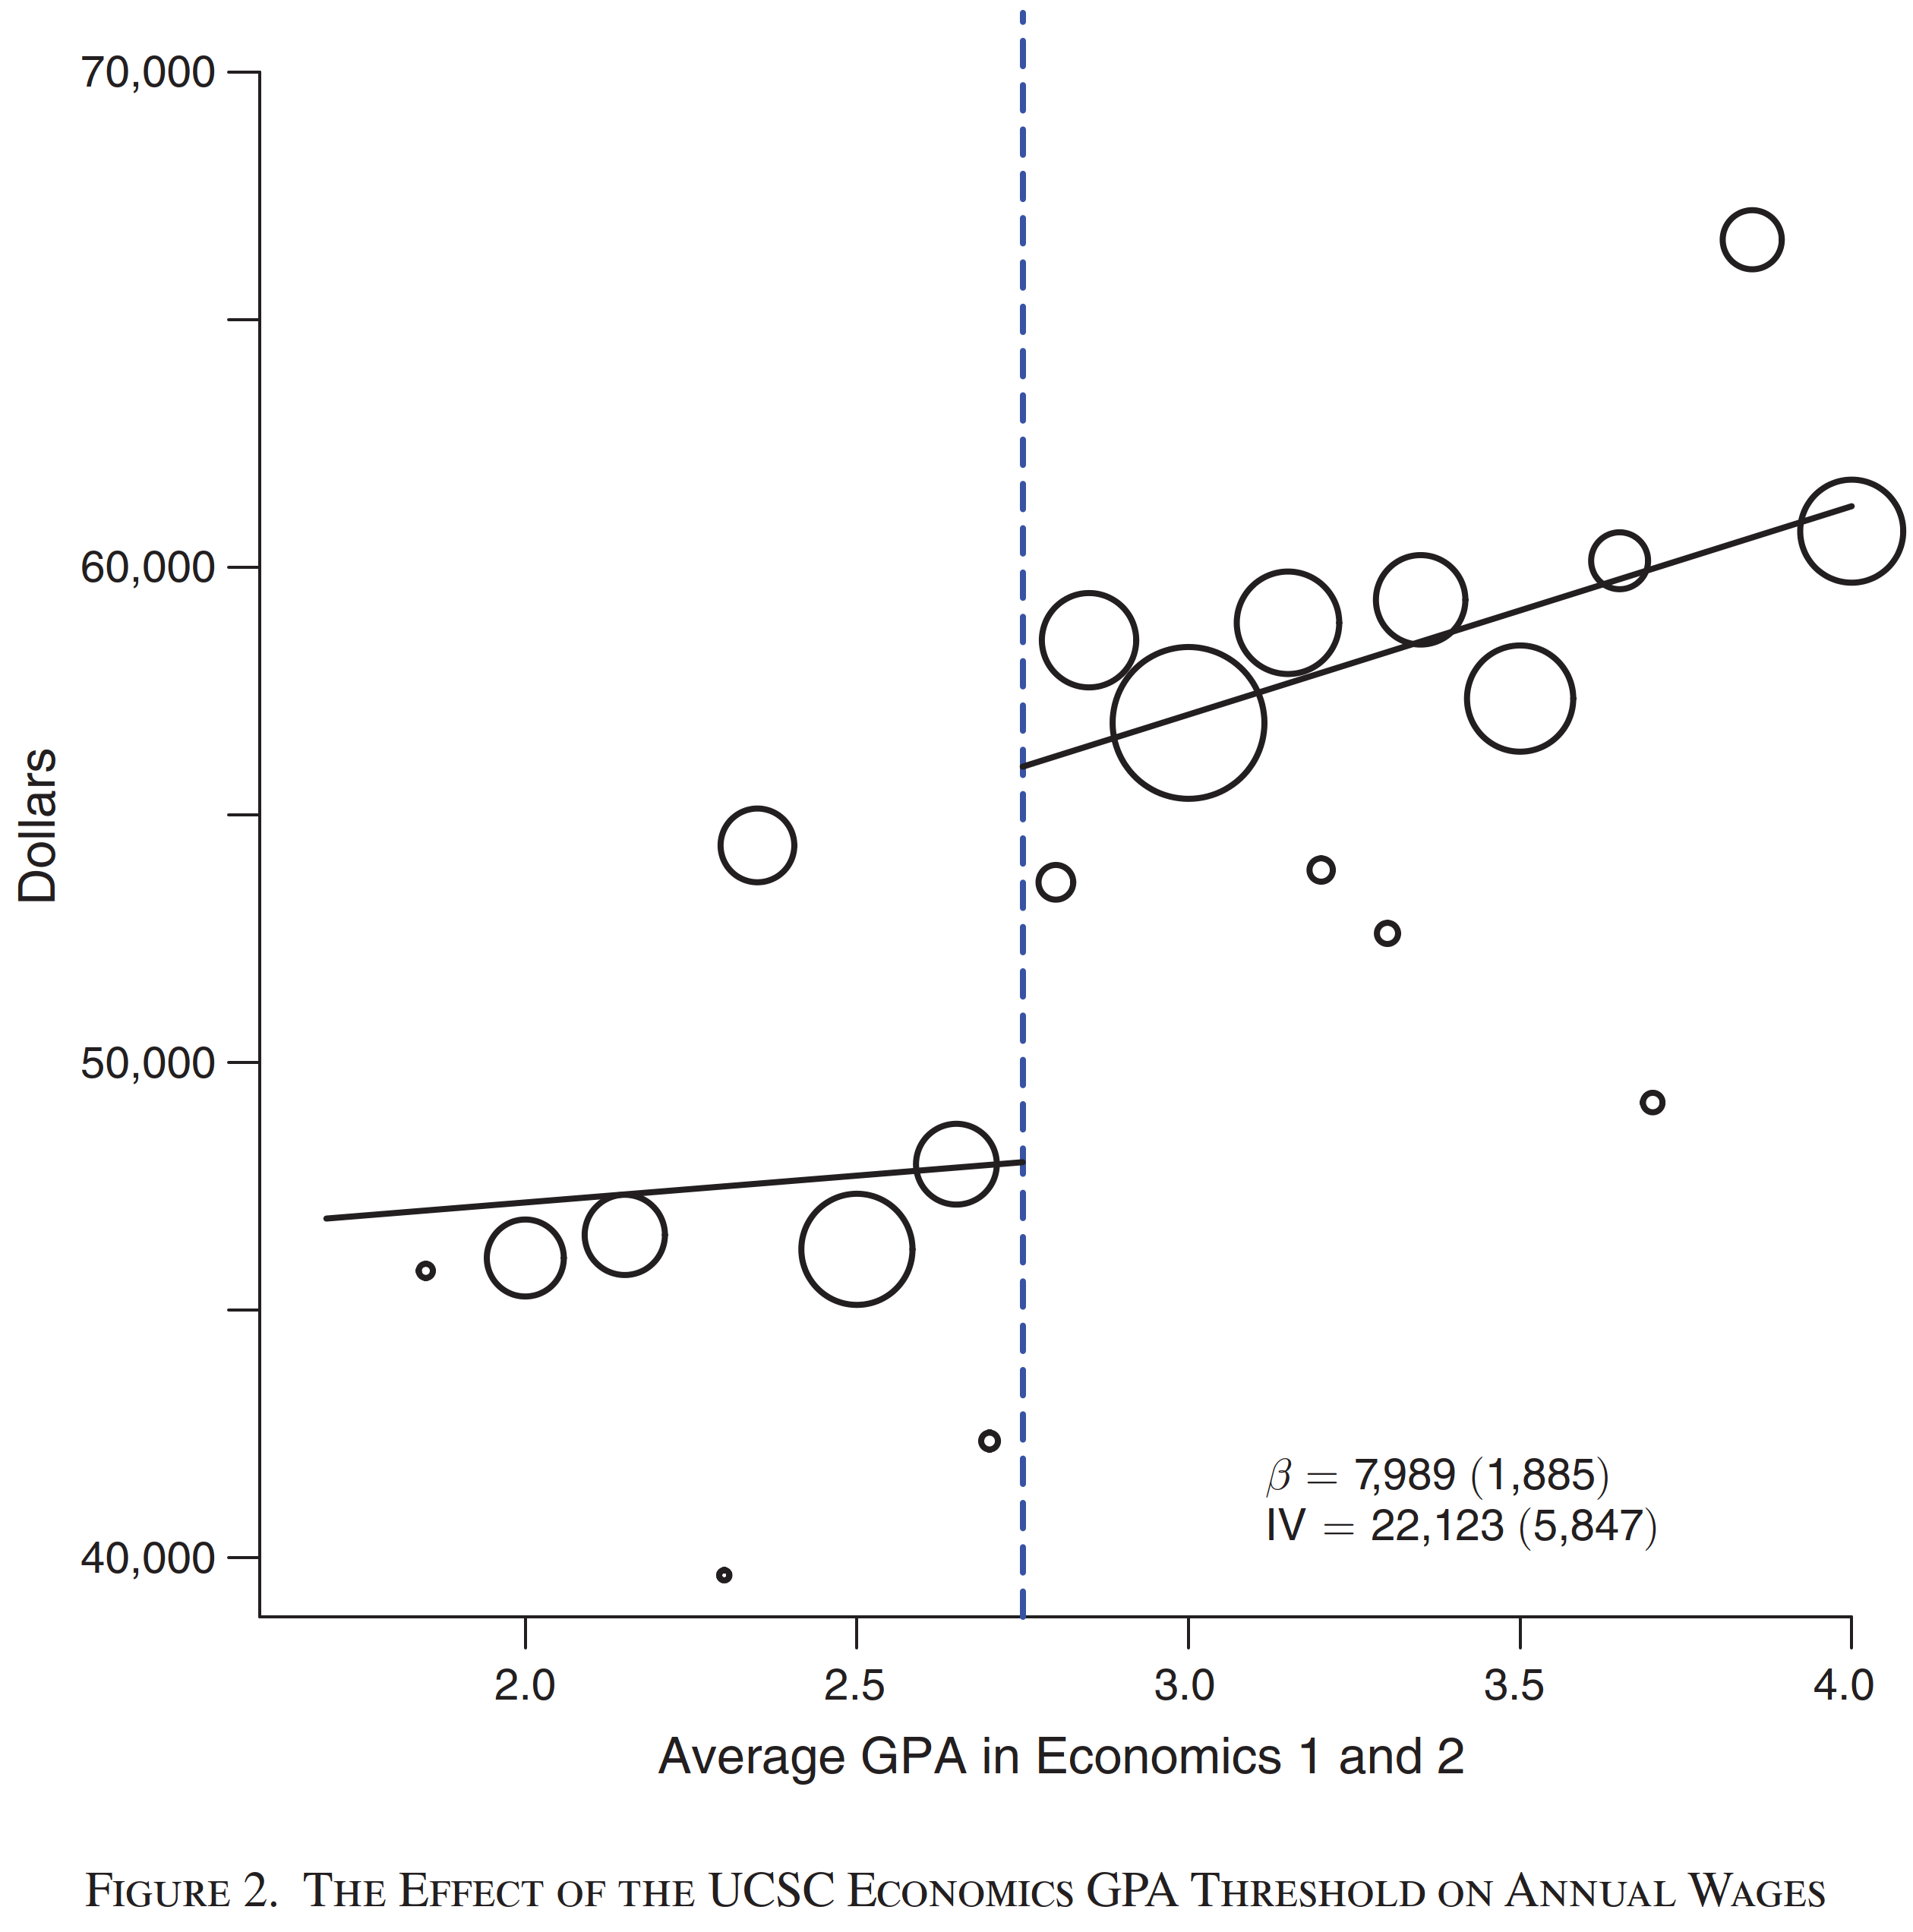
\includegraphics[width=0.60\textwidth]{figure/RD_econ_major_f2.png}
	
	
\end{frame}



\begin{frame}{Empirical Example: Bleemer \& Mehta (2022)}{Key Findings}
	\begin{itemize}
		\item \textbf{Large Returns}: Majoring in economics caused:
							\vspace{0.2cm}
		\begin{itemize}
			\item 46\% increase in early-career wages (\$22,000)
								\vspace{0.2cm}
			\item Similar effects for male and female students
								\vspace{0.2cm}
			\item Possibly larger effects for URM students
											\vspace{0.2cm}
					\begin{itemize}
			\item URM: Underrepresented Minority includes Black, Hispanic, and Native American students
					\end{itemize}
		\end{itemize}
		
		\vspace{0.2cm}
%		\item \textbf{Important Implications}:
%		\begin{itemize}
%			\item Major choice is first-order determinant of returns to college
%			\item Returns primarily through industry sorting
%			\item University policies affecting major access have important mobility implications
%			\item Wage differences by major approximate causal effects
%		\end{itemize}
	\end{itemize}
\end{frame}



\begin{frame}{Empirical Example: Bleemer \& Mehta (2022)}{Mechanisms: Educational Investment}
	
	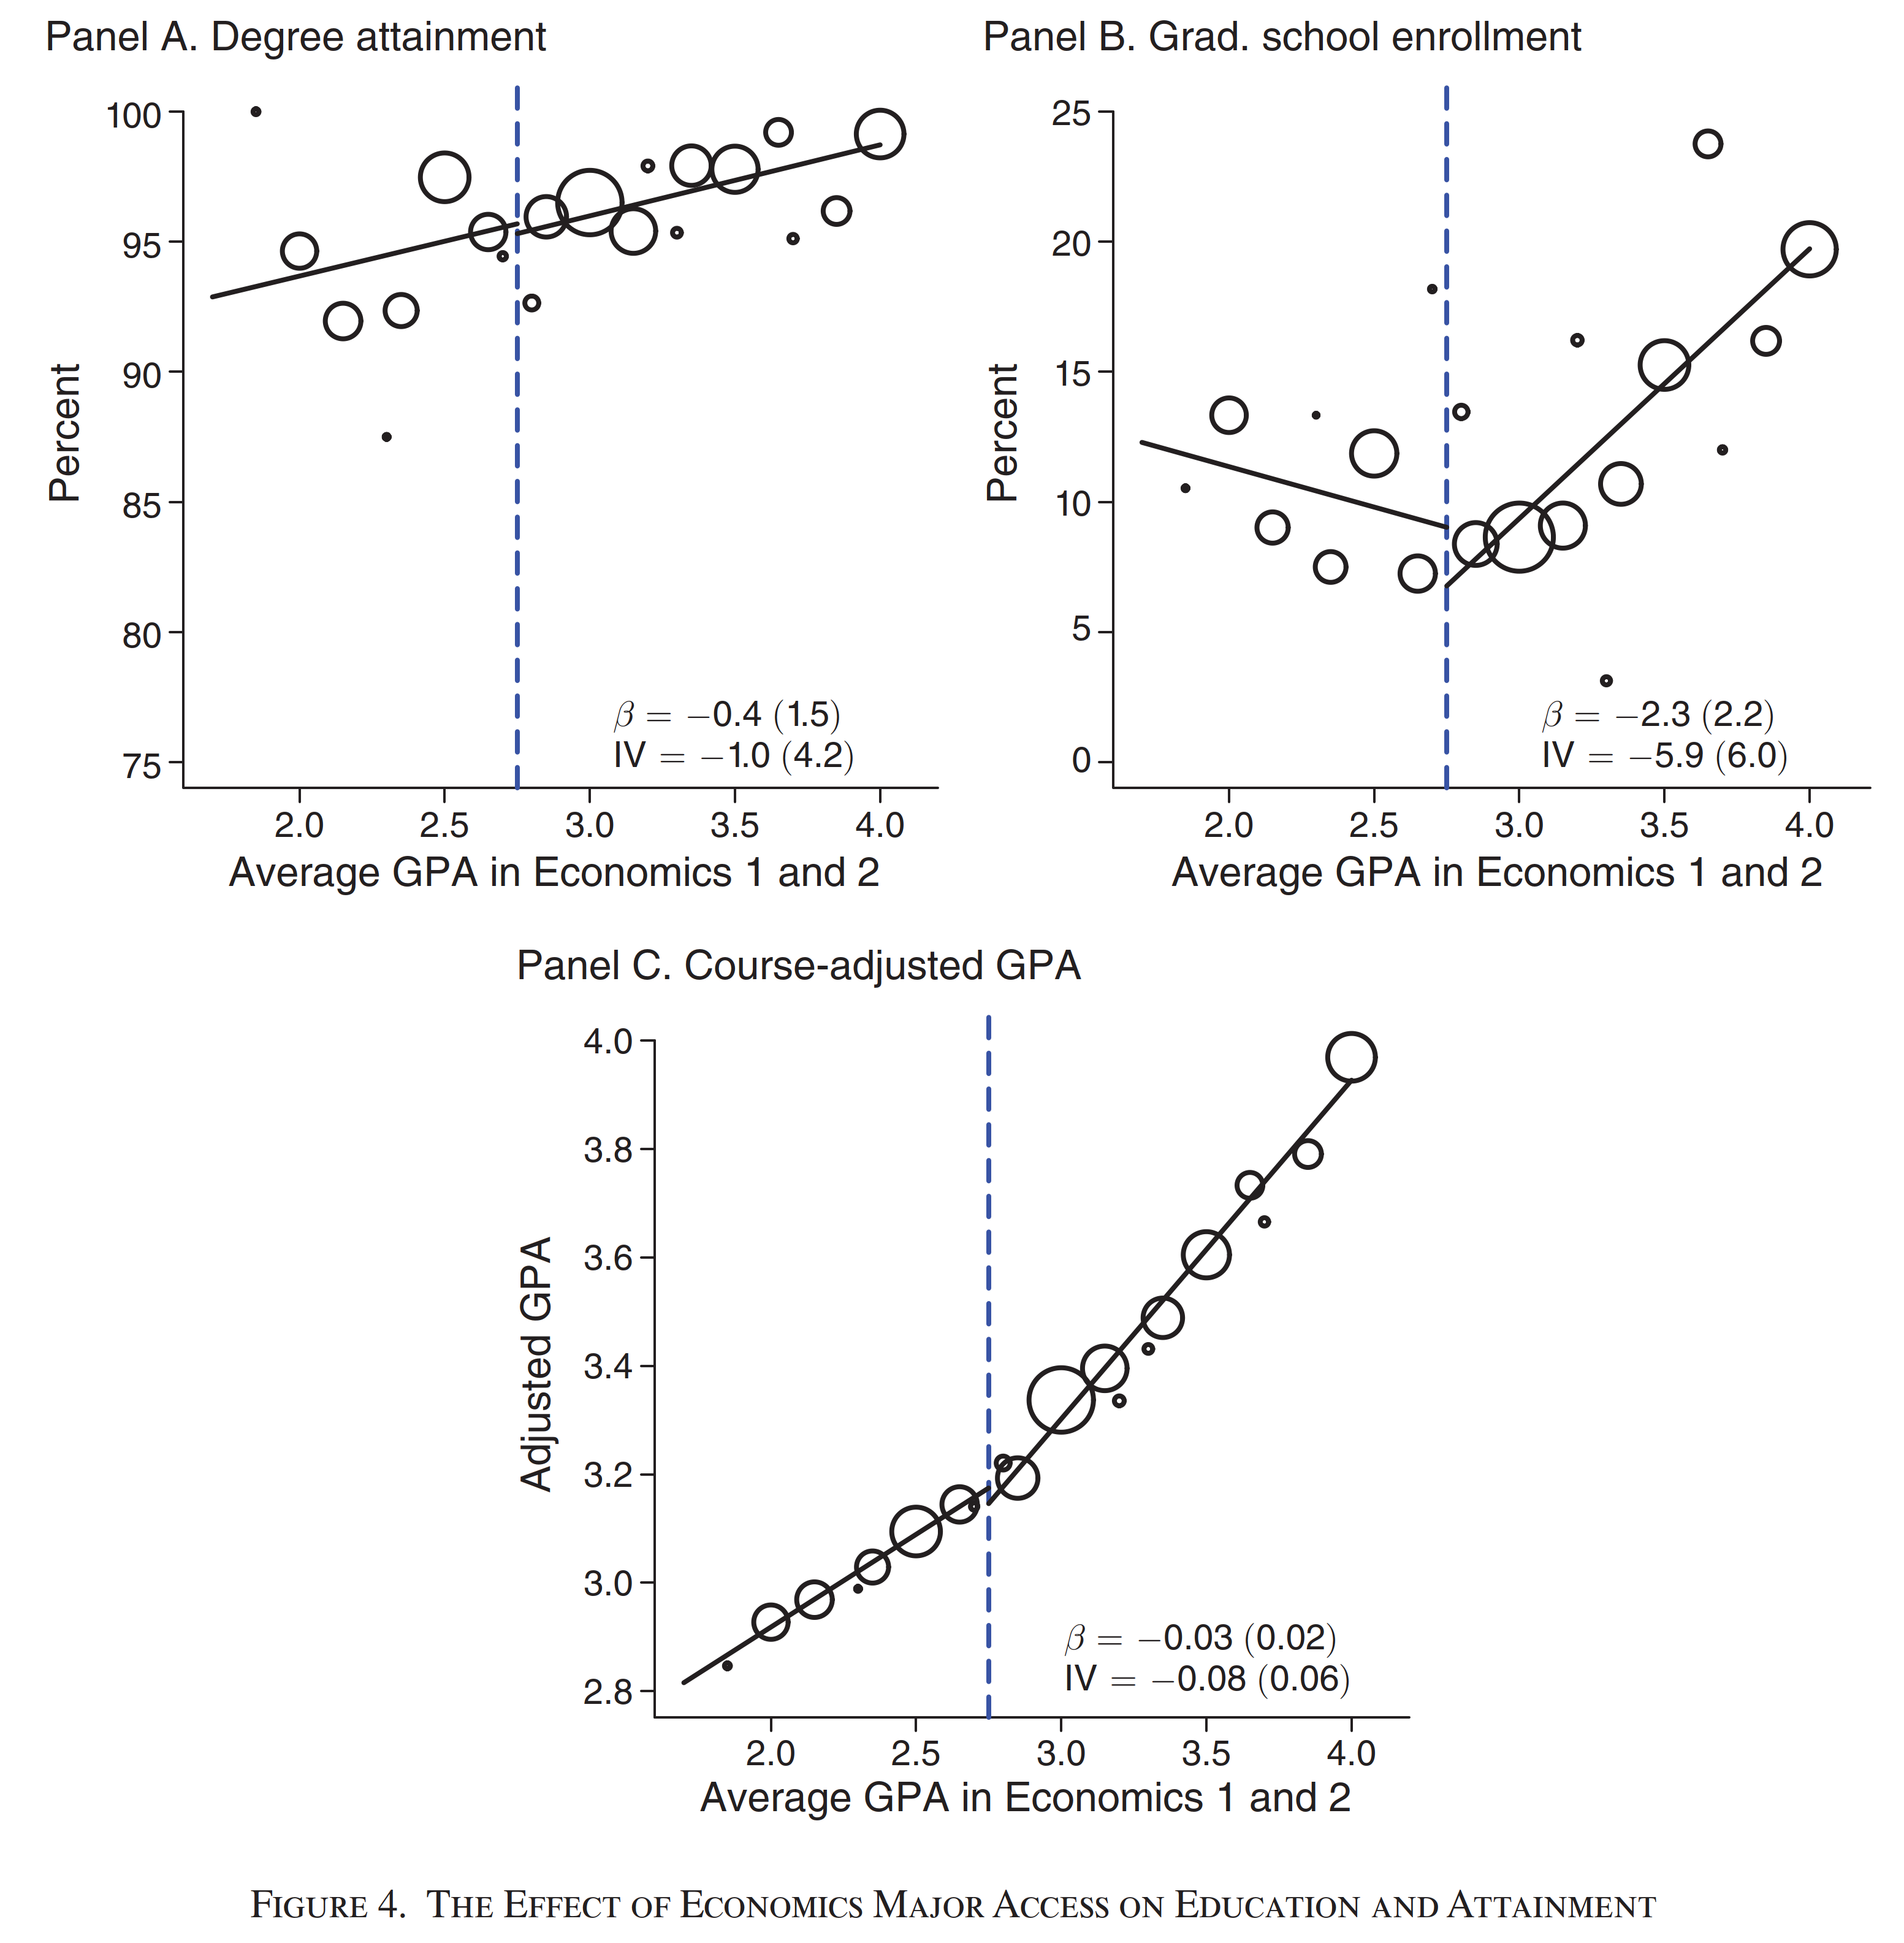
\includegraphics[width=0.7\textwidth]{figure/RD_econ_major_f3.png}
	
	
\end{frame}



\begin{frame}{Empirical Example: Bleemer \& Mehta (2022)}{Mechanisms: Industry Effects}
	
	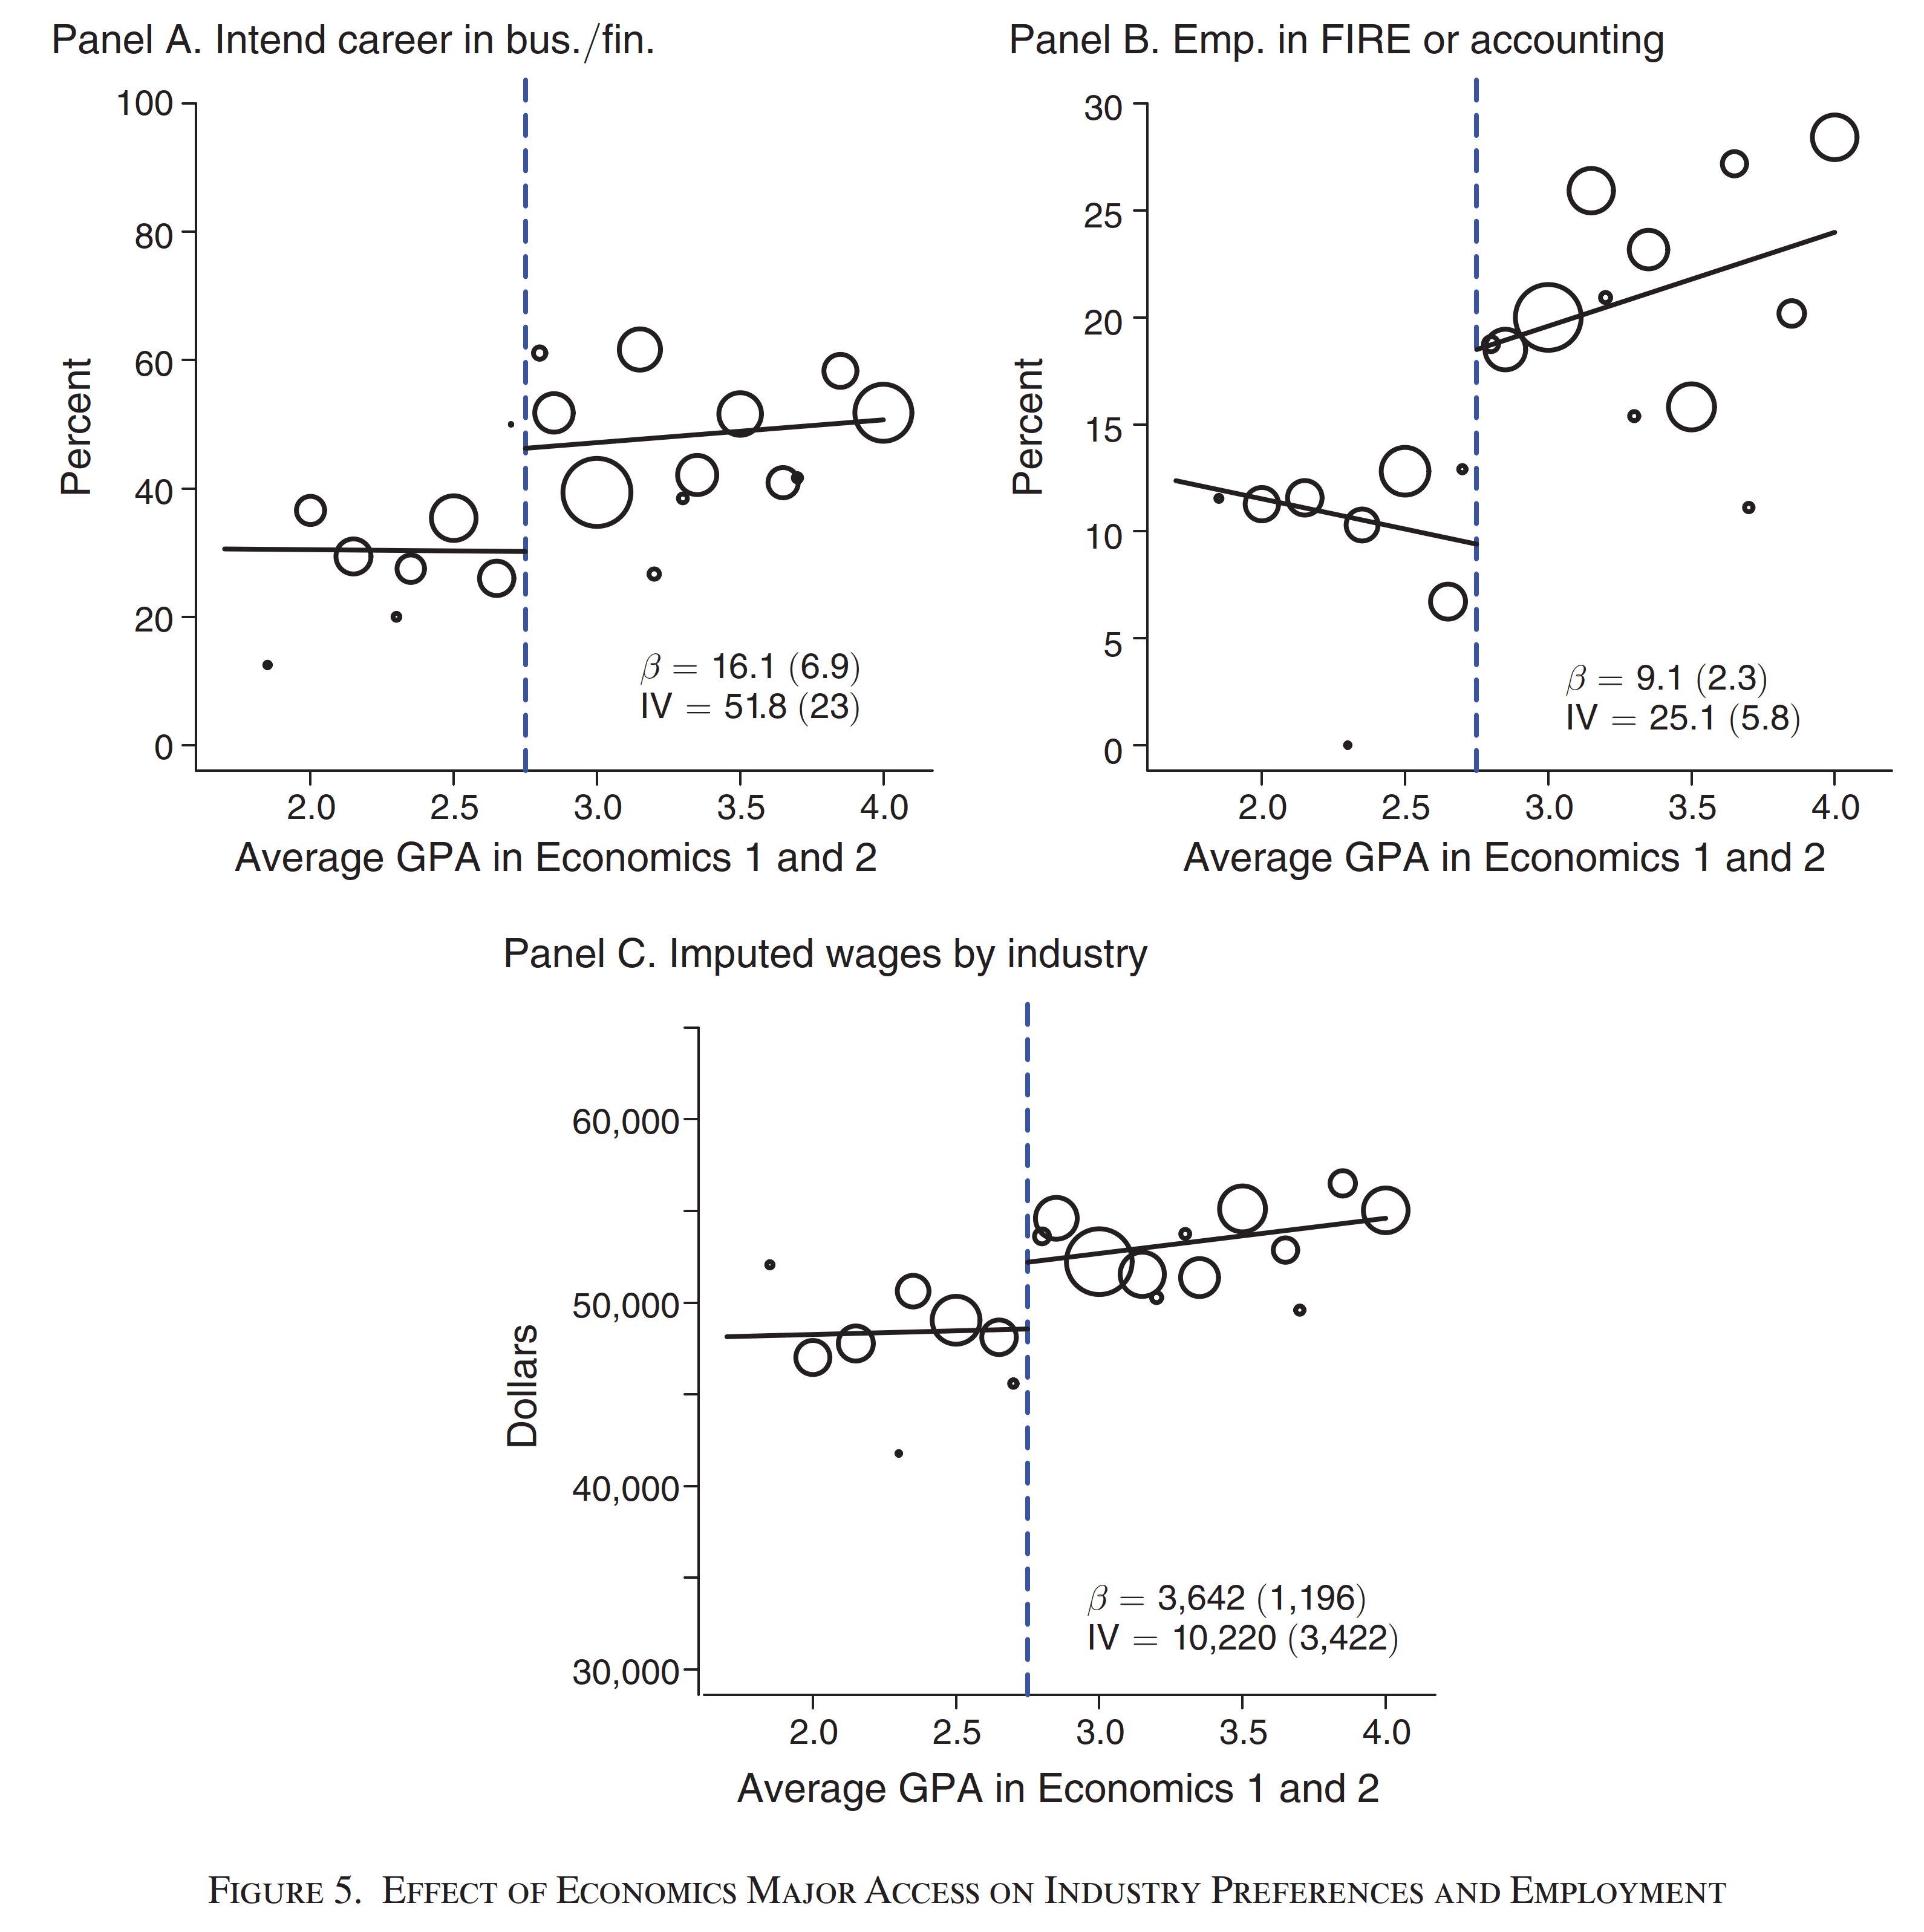
\includegraphics[width=0.7\textwidth]{figure/RD_econ_major_f4.png}
	
	
\end{frame}




\begin{frame}{Empirical Example: Bleemer \& Mehta (2022)}{Mechanisms}
	\begin{itemize}
		\item \textbf{Educational Investment}:
										\vspace{0.2cm}
		\begin{itemize}
			\item No effect on graduation rates or graduate school enrollment
											\vspace{0.2cm}
			\item No change in study time or course-adjusted grades
											\vspace{0.2cm}
			\item 13 more economics courses, 9 fewer other social science courses
											\vspace{0.2cm}
		\end{itemize}
		
		\vspace{0.2cm}
		\item \textbf{Industry Effects}:
										\vspace{0.2cm}
		\begin{itemize}
			\item 52 pp more likely to prefer business/finance careers
											\vspace{0.2cm}
			\item 25 pp more likely to work in FIRE or accounting
											\vspace{0.2cm}
			\item About half (\$10,220) of wage effect explained by industry sorting
		\end{itemize}
		
		\vspace{0.2cm}
%		\item \textbf{Observational vs. Causal Effects}:
%		\begin{itemize}
%			\item OLS estimates slightly underestimate true returns
%			\item Suggests selection bias is small in this context
%		\end{itemize}
	\end{itemize}
\end{frame}






\begin{frame}{Empirical Example: Bleemer \& Mehta (2022)}{Alternative Specifications}
	\begin{itemize}
	
		\item \textbf{Robustness Checks}:
		\begin{enumerate}
			\item Quadratic running variable terms
			\item Adding controls:
			\begin{itemize}
				\item Demographic variables
				\item High school fixed effects
			\end{itemize}
			\item Narrower bandwidth (±0.5 GPA points)
			%\item Honest RD with optimal bandwidth (Kolesár \& Rothe, 2018)
		\end{enumerate}
		
		\vspace{0.2cm}
		\item Results robust across all specifications
	\end{itemize}
\end{frame}


\begin{frame}{Suggested Readings} % Changed title to reflect RDD
	\begin{itemize} 
		\item Chapter 4, \textit{Mastering 'Metrics: The Path from Cause to Effect}
		\vspace{0.2cm}
		\item Chapter 6, \textit{Mostly Harmless Econometrics: An Empiricist's Companion} % Added "An Empiricist's Companion" for completeness
		\vspace{0.2cm}
		\item Chapter 6, \textit{Causal Inference: The Mixtape}
	\end{itemize}
\end{frame}





% ================================================================
% Stata Example: Bleemer & Mehta (2022) -- Fuzzy RDD
% Mirrors the Lee-Moretti-Butler election example style
% ================================================================

\title[]
{Stata Example: Fuzzy RDD}

\author
{}

\institute{}

\date
{}

\begin{frame}{}
	\titlepage
\end{frame}


\begin{frame}{Bleemer \& Mehta (2022)}{Overview}

	Zachary Bleemer and Aashish Mehta (2022) ``\textbf{Will Studying Economics Make You Rich? A Regression Discontinuity Analysis of the Returns to College Major}'' \textit{American Economic Journal: Applied Economics}

	\vspace{0.2cm}
	\begin{itemize}
		\item Estimate the \textbf{causal effect} of majoring in economics on early-career wages
		\vspace{0.2cm}
		\item UC Santa Cruz restricted access to the economics major:
		\begin{itemize}
			\vspace{0.2cm}
			\item Students needed GPA $\geq 2.8$ in Economics 1 \& 2 to declare the major
			\vspace{0.2cm}
		\end{itemize}
		\item OLS overstates the economics premium because high-ability students
		\textbf{both} self-select into economics \textbf{and} earn higher wages
		\vspace{0.2cm}
		\item We use \textbf{simulated data} (N = 4,000) calibrated to the paper:
		\begin{itemize}
			\vspace{0.2cm}
			\item First stage $\approx$ 36 pp; LATE $\approx$ 46\% wage premium (\$22,000/year)
		\end{itemize}
	\end{itemize}
\end{frame}


\begin{frame}{Bleemer \& Mehta (2022)}{Identification Strategy}
	\begin{itemize}
		\item \textbf{Fuzzy RDD}: GPA cutoff at 2.8 is the instrument $Z_i$ for economics major $D_i$
		\vspace{0.2cm}
		\item Crossing the cutoff \emph{shifts} but does not \emph{determine} major choice
		\begin{itemize}
			\vspace{0.2cm}
			\item Students above cutoff may still choose other majors (never-takers)
			\item Students below cutoff sometimes declare economics anyway (always-takers)
		\end{itemize}
		\vspace{0.2cm}
		\item \textbf{Key idea}: near the cutoff, being above vs.\ below is as good as random
		\begin{itemize}
			\vspace{0.2cm}
			\item Students just above/below GPA 2.8 are otherwise comparable
		\end{itemize}
	\end{itemize}
\end{frame}


\begin{frame}{Bleemer \& Mehta (2022)}{Identification Strategy}

	\begin{equation*}
	\begin{aligned}
	D_i &= \alpha_1 + \rho_1 Z_i + \mathrm{f}_1(A_i) + \upsilon_i \qquad \text{(First Stage)}\\
	Y_i &= \alpha_2 + \rho_2 D_i + \mathrm{f}_2(A_i) + \eta_i \qquad\;\, \text{(Second Stage)}
	\end{aligned}
	\end{equation*}

	\begin{itemize}
		\item $Y_i$ (outcome): log average wages 2017--2018
		\vspace{0.2cm}
		\item $A_i$ (running variable): GPA in Economics 1 \& 2
		\vspace{0.2cm}
		\item $Z_i = \mathbf{1}[A_i \geq 2.8]$ (eligibility / instrument)
		\vspace{0.2cm}
		\item $D_i$ (treatment): 1 if student majored in economics
		\vspace{0.2cm}
		\item LATE $= \rho_2 = \rho_2^{\text{RF}} / \rho_1^{\text{FS}}$
		(causal effect for \textbf{compliers} at the cutoff)
	\end{itemize}
\end{frame}


\begin{frame}{Bleemer \& Mehta (2022)}{STATA Implementation}
	\begin{itemize}
		\item See \texttt{exercise\_stata\_econ\_rdd.do}
		\vspace{0.2cm}
		\item Use \texttt{simulated\_econ\_rdd.dta}
		\vspace{0.2cm}
		\item Install the following ado files:
		\begin{itemize}
			\vspace{0.2cm}
			\item \texttt{binscatter.ado}
			\item \texttt{rdrobust.ado}
			\item \texttt{rddensity.ado}
			\item \texttt{DCdensity.ado}
		\end{itemize}
	\end{itemize}
\end{frame}


%------------------------------------------------------------
% STEP 1: Graphical Analysis
%------------------------------------------------------------

\begin{frame}{Step 1: Graphical Analysis}{First Stage}
	\begin{itemize}
		\item In fuzzy RDD we always plot \textbf{two} graphs -- first stage and reduced form
		\vspace{0.2cm}
		\item \textbf{First stage}: plot the \textbf{treatment} ($D_i$ = economics major)
		by the \textbf{running variable} ($A_i$ = GPA)
		\vspace{0.2cm}
		\begin{itemize}
			\item Construct bins and average the treatment within bins on both sides of the cutoff
			\vspace{0.2cm}
			\item Inspect whether the probability of economics major \textbf{jumps} at GPA = 2.8
			\vspace{0.2cm}
			\item The size of the jump is the \textbf{first-stage estimate}
		\end{itemize}
	\end{itemize}
\end{frame}


\begin{frame}[fragile]{STATA Command: binscatter}{First Stage}
	\begin{itemize}
		\item Example (first stage graph):
\begin{lstlisting}
use "simulated_econ_rdd.dta", clear
binscatter econ_major gpa_econ, n(50) rd(2.8) linetype(lfit)
graph export figure/econ_fs.png, replace
\end{lstlisting}
		\vspace{0.2cm}
		\item \textbf{econ\_major}: treatment variable $D_i$ on the y-axis
		\vspace{0.2cm}
		\item \textbf{gpa\_econ}: running variable $A_i$ on the x-axis
		\vspace{0.2cm}
		\item \textbf{rd(2.8)}: split the sample at the GPA cutoff
		\vspace{0.2cm}
		\item \textbf{linetype(lfit)}: fit a linear regression line on each side
	\end{itemize}
\end{frame}


\begin{frame}{First Stage}{P(Economics Major) by GPA in Introductory Economics}

	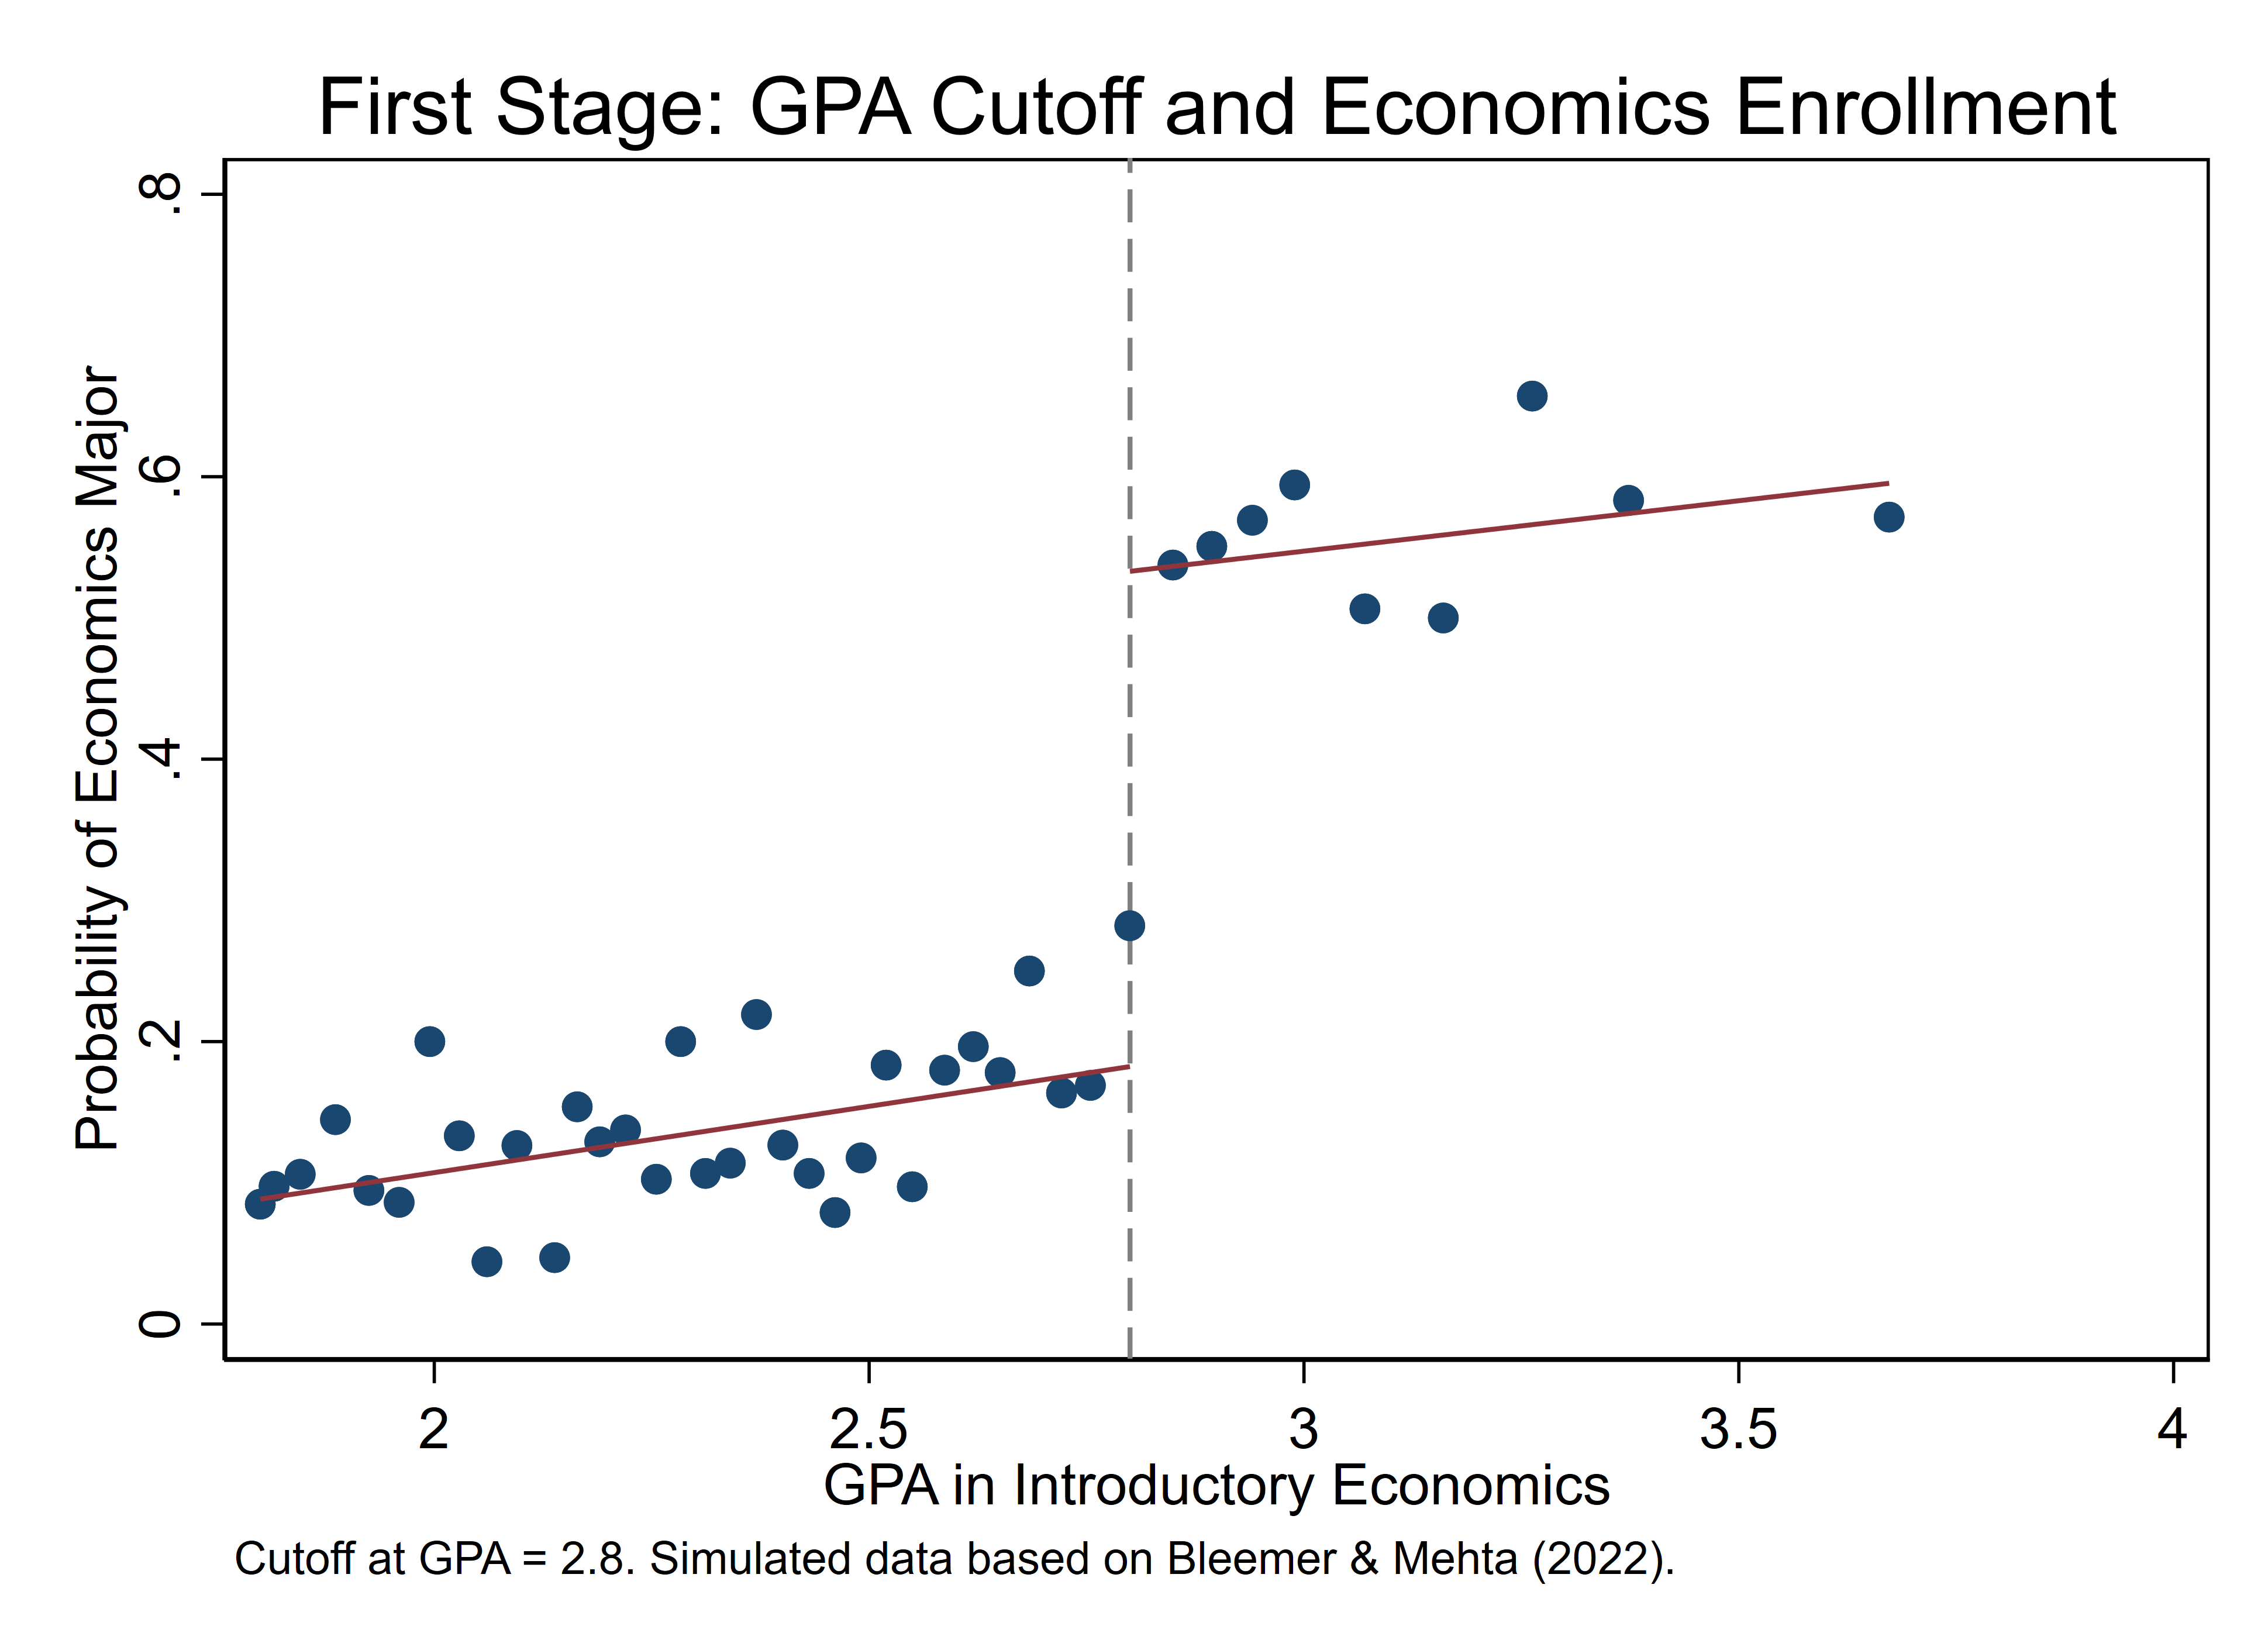
\includegraphics[width=0.9\textwidth]{figure/econ_fs.png}

\end{frame}


\begin{frame}{Step 1: Graphical Analysis}{Reduced Form}
	\begin{itemize}
		\item \textbf{Reduced form}: plot the \textbf{outcome} ($Y_i$ = log wages)
		by the \textbf{running variable} ($A_i$ = GPA)
		\vspace{0.2cm}
		\begin{itemize}
			\item This shows the \textbf{intent-to-treat (ITT)} effect:
			the total effect of \emph{eligibility} on wages
			\vspace{0.2cm}
			\item The jump at GPA = 2.8 is the \textbf{reduced-form estimate}
			\vspace{0.2cm}
			\item LATE = Reduced Form / First Stage
		\end{itemize}
	\end{itemize}
\end{frame}


\begin{frame}[fragile]{STATA Command: binscatter}{Reduced Form}
	\begin{itemize}
		\item Example (reduced form graph):
\begin{lstlisting}
binscatter logwage_1718 gpa_econ if employed_1718,
    n(50) rd(2.8) linetype(lfit)
graph export figure/econ_rf.png, replace
\end{lstlisting}
		\vspace{0.2cm}
		\item \textbf{logwage\_1718}: outcome variable $Y_i$ on the y-axis
		\vspace{0.2cm}
		\item \textbf{if employed\_1718}: restrict to employed workers
		(wages only observed for employed)
		\vspace{0.2cm}
		\item A visible jump at GPA = 2.8 indicates that the GPA cutoff
		affects wages through the economics major pathway
	\end{itemize}
\end{frame}


\begin{frame}{Reduced Form}{Log Wages by GPA in Introductory Economics}

	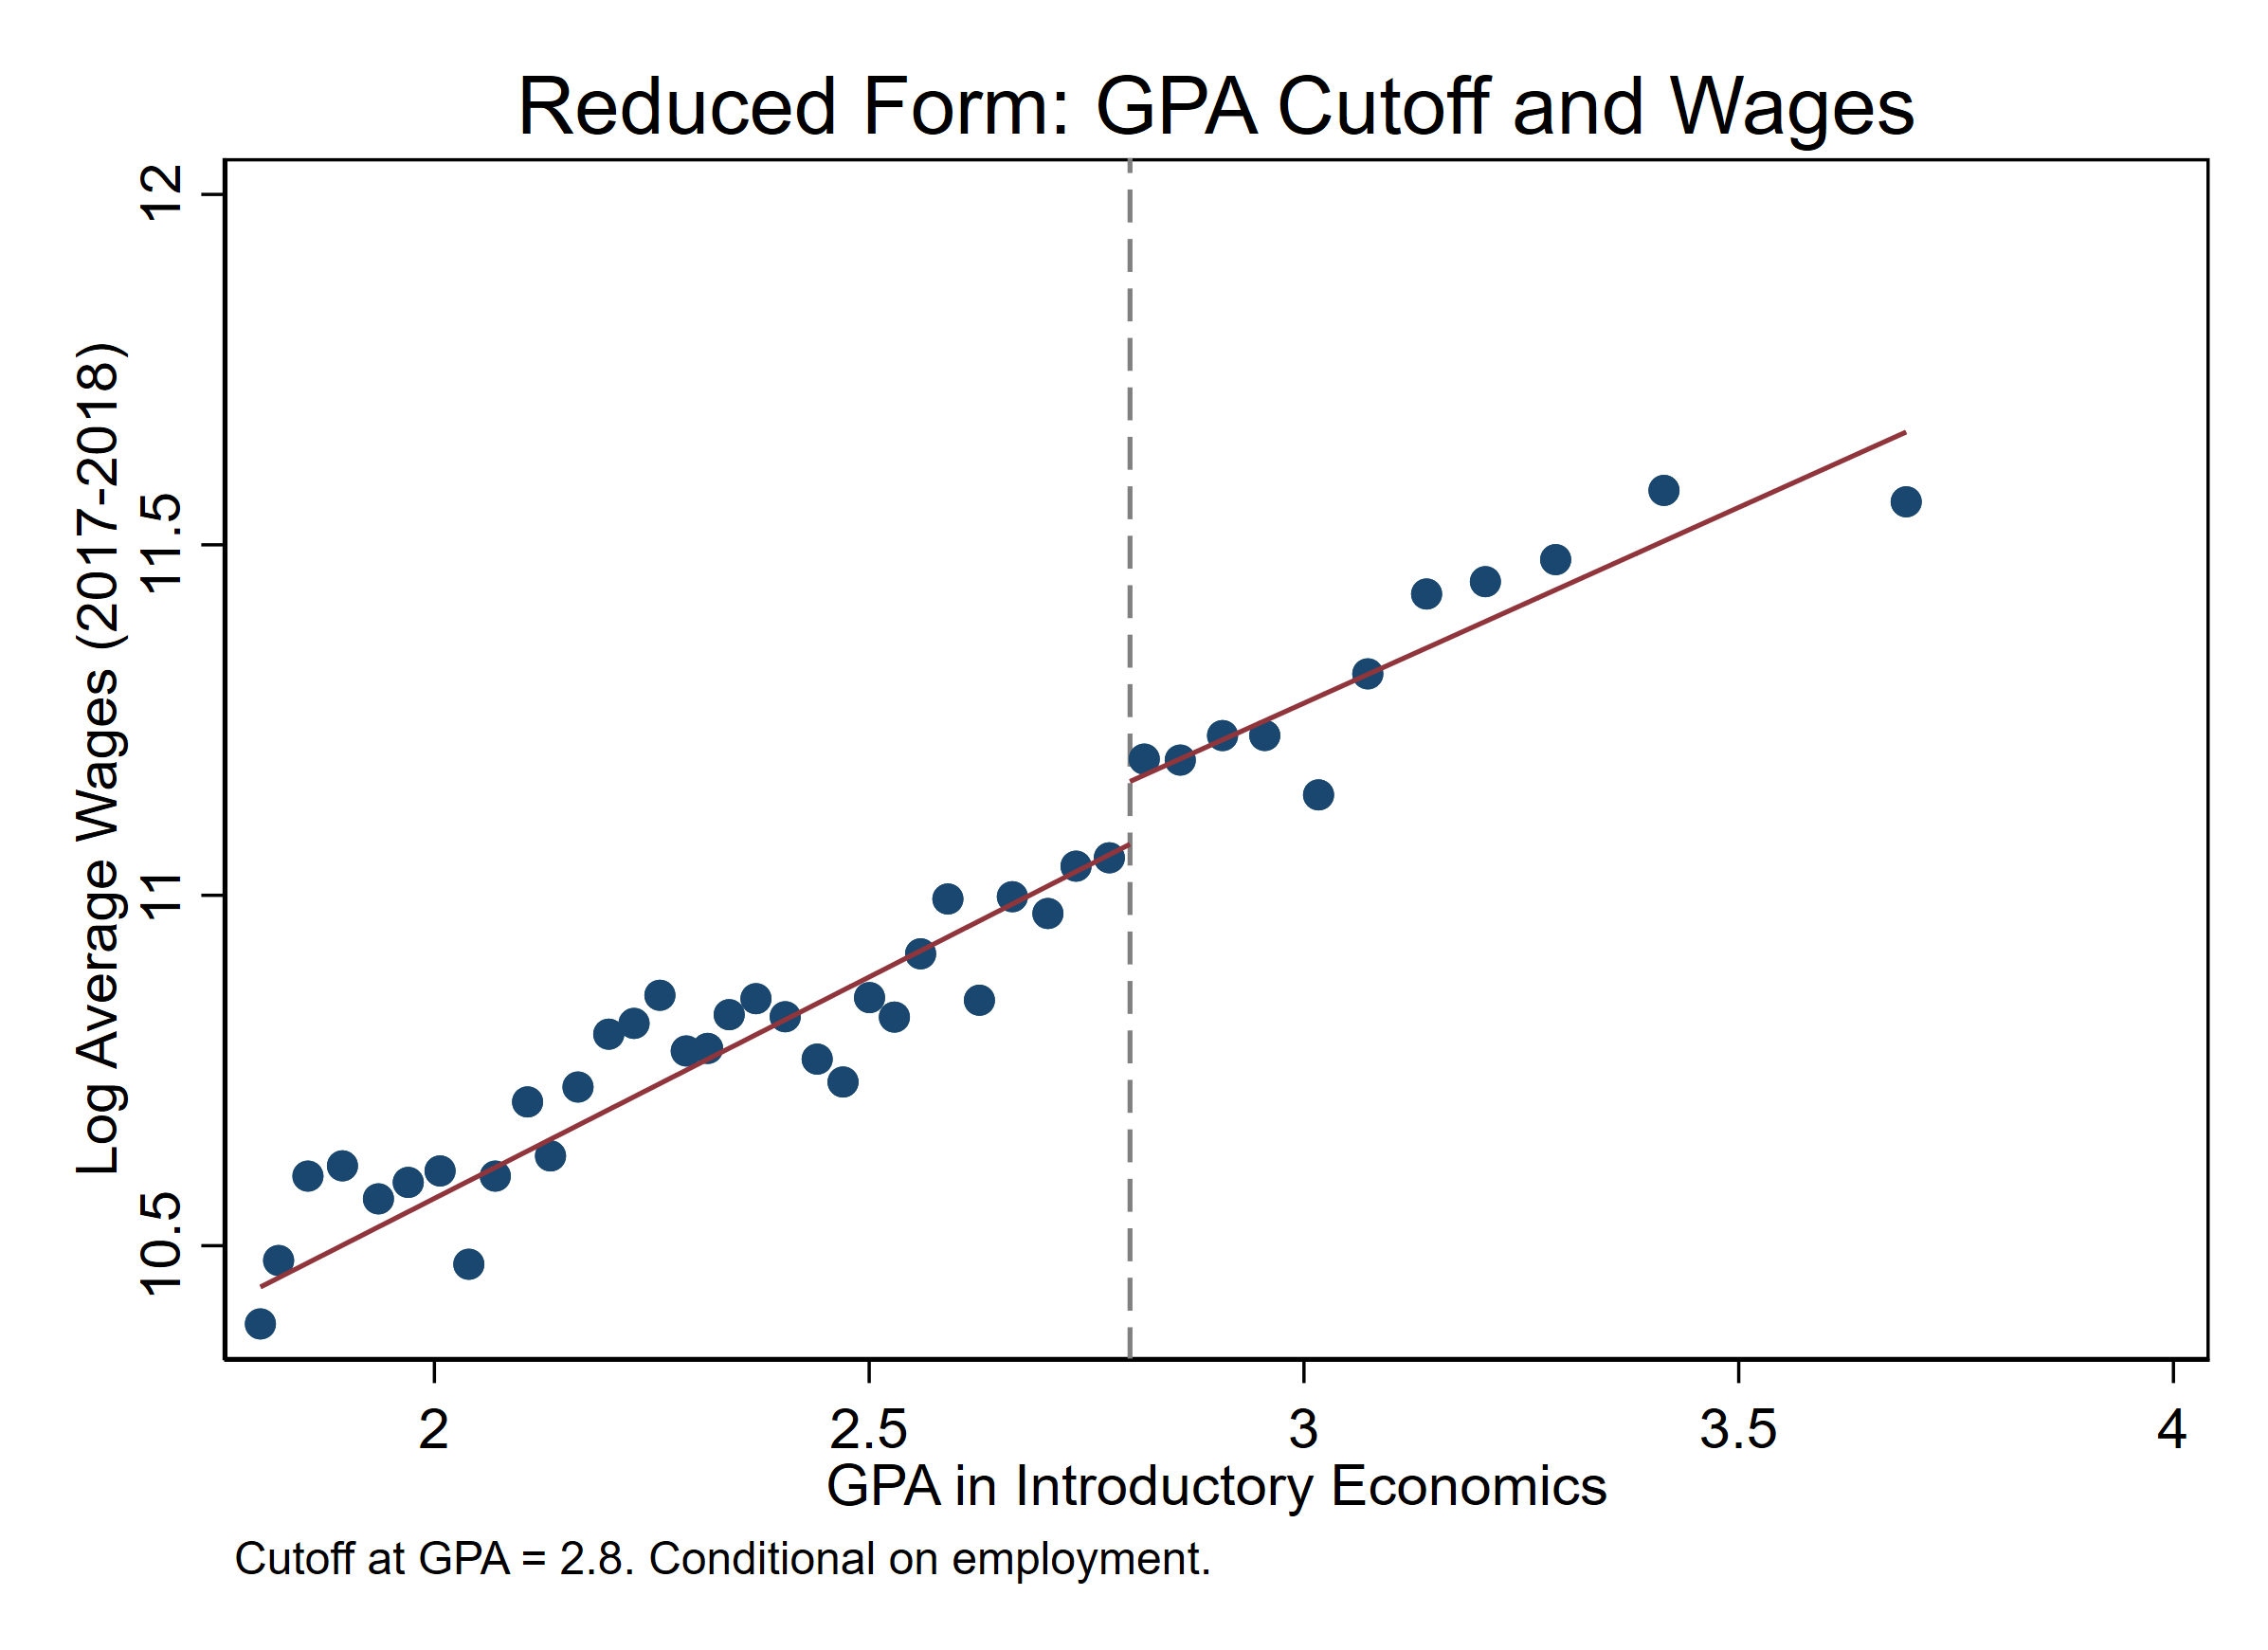
\includegraphics[width=0.9\textwidth]{figure/econ_rf.png}

\end{frame}


\begin{frame}{Step 1: Graphical Analysis}{Covariate Balance}
	\begin{itemize}
		\item Construct a similar graph but using \textbf{pre-determined covariates}
		as the ``outcome''
		\vspace{0.2cm}
		\item Pre-determined variables should show \textbf{no discontinuity} at the cutoff
		\vspace{0.2cm}
		\begin{itemize}
			\item These variables are fixed before students know their intro econ GPA
			\vspace{0.2cm}
			\item If a covariate jumps at GPA 2.8, students above/below are
			systematically different $\Rightarrow$ threat to the continuity assumption
		\end{itemize}
		\vspace{0.2cm}
		\item Check: \texttt{sat\_score}, \texttt{female}, \texttt{urm}, \texttt{zip\_income}
	\end{itemize}
\end{frame}


\begin{frame}[fragile]{STATA Command: binscatter}{Covariate Balance}
	\begin{itemize}
		\item Example (SAT score balance):
\begin{lstlisting}
binscatter sat_score gpa_econ, n(50) rd(2.8) linetype(lfit)
graph export figure/econ_sat.png, replace

binscatter female gpa_econ, n(50) rd(2.8) linetype(lfit)
graph export figure/econ_female.png, replace

binscatter urm gpa_econ, n(50) rd(2.8) linetype(lfit)
graph export figure/econ_urm.png, replace
\end{lstlisting}
	\end{itemize}
\end{frame}


\begin{frame}{Covariate Balance}{SAT Score by GPA in Introductory Economics}

	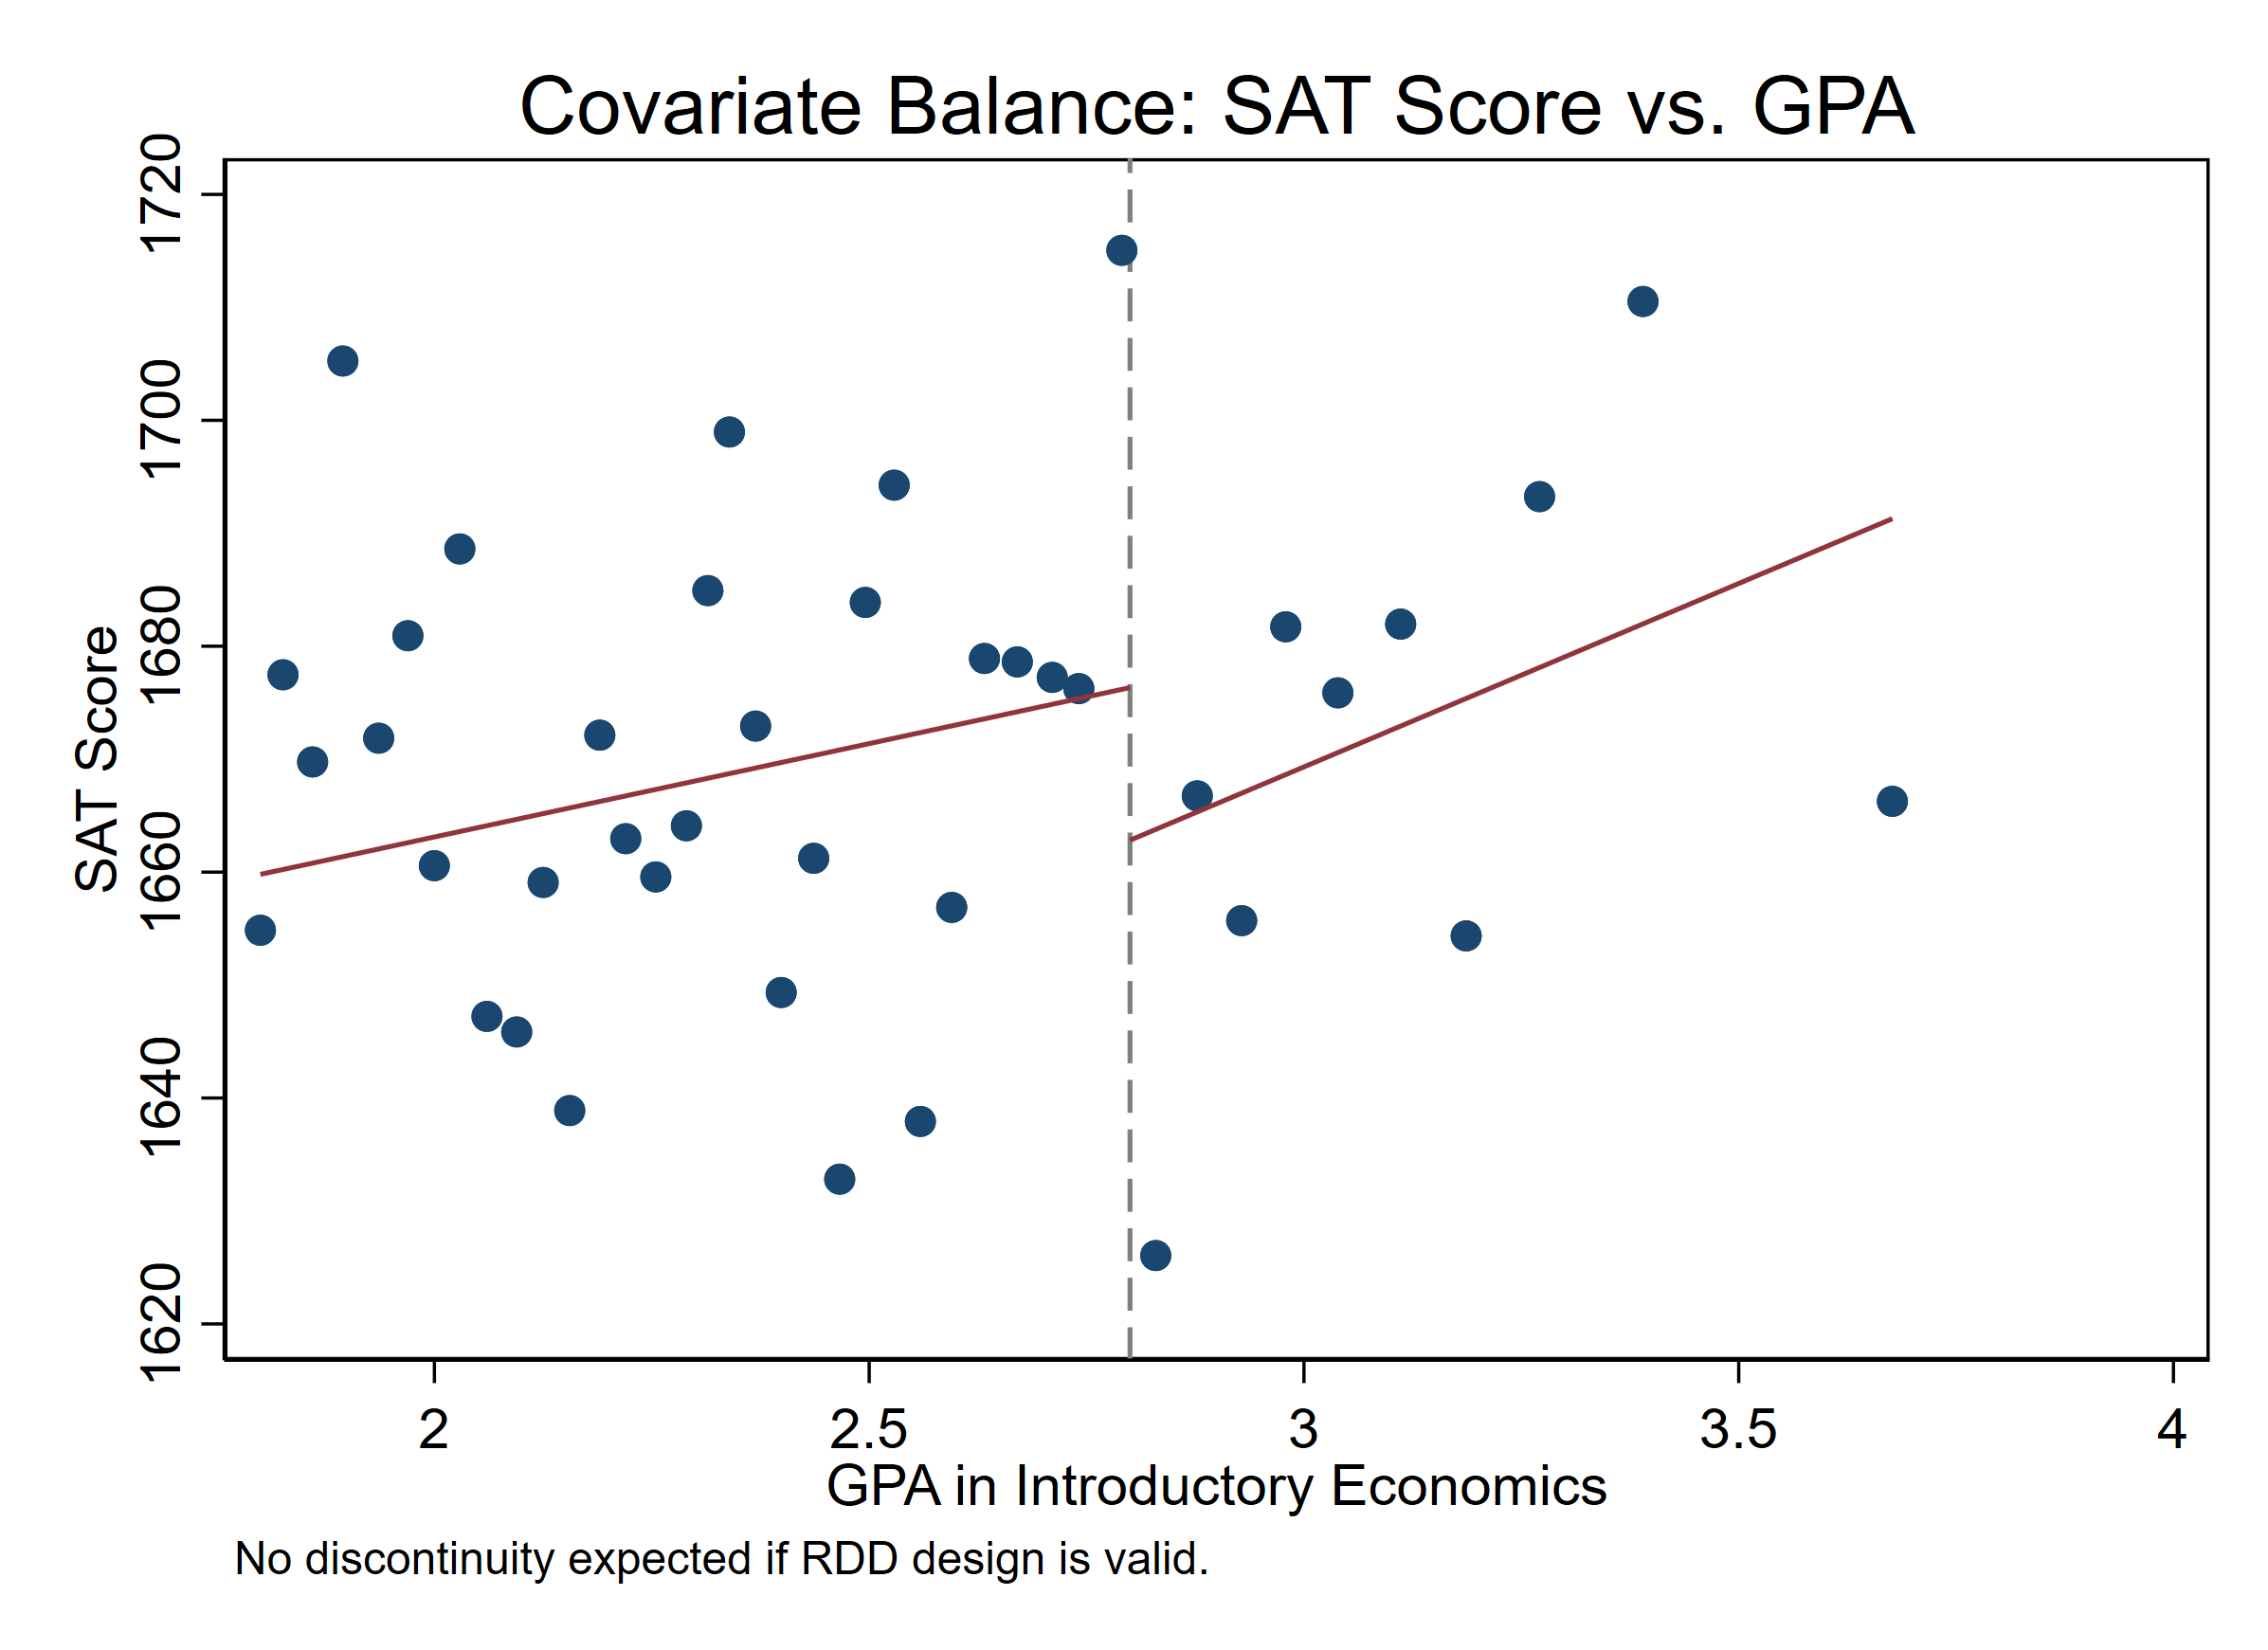
\includegraphics[width=0.9\textwidth]{figure/econ_sat.png}

\end{frame}


\begin{frame}{Covariate Balance}{Female by GPA in Introductory Economics}

	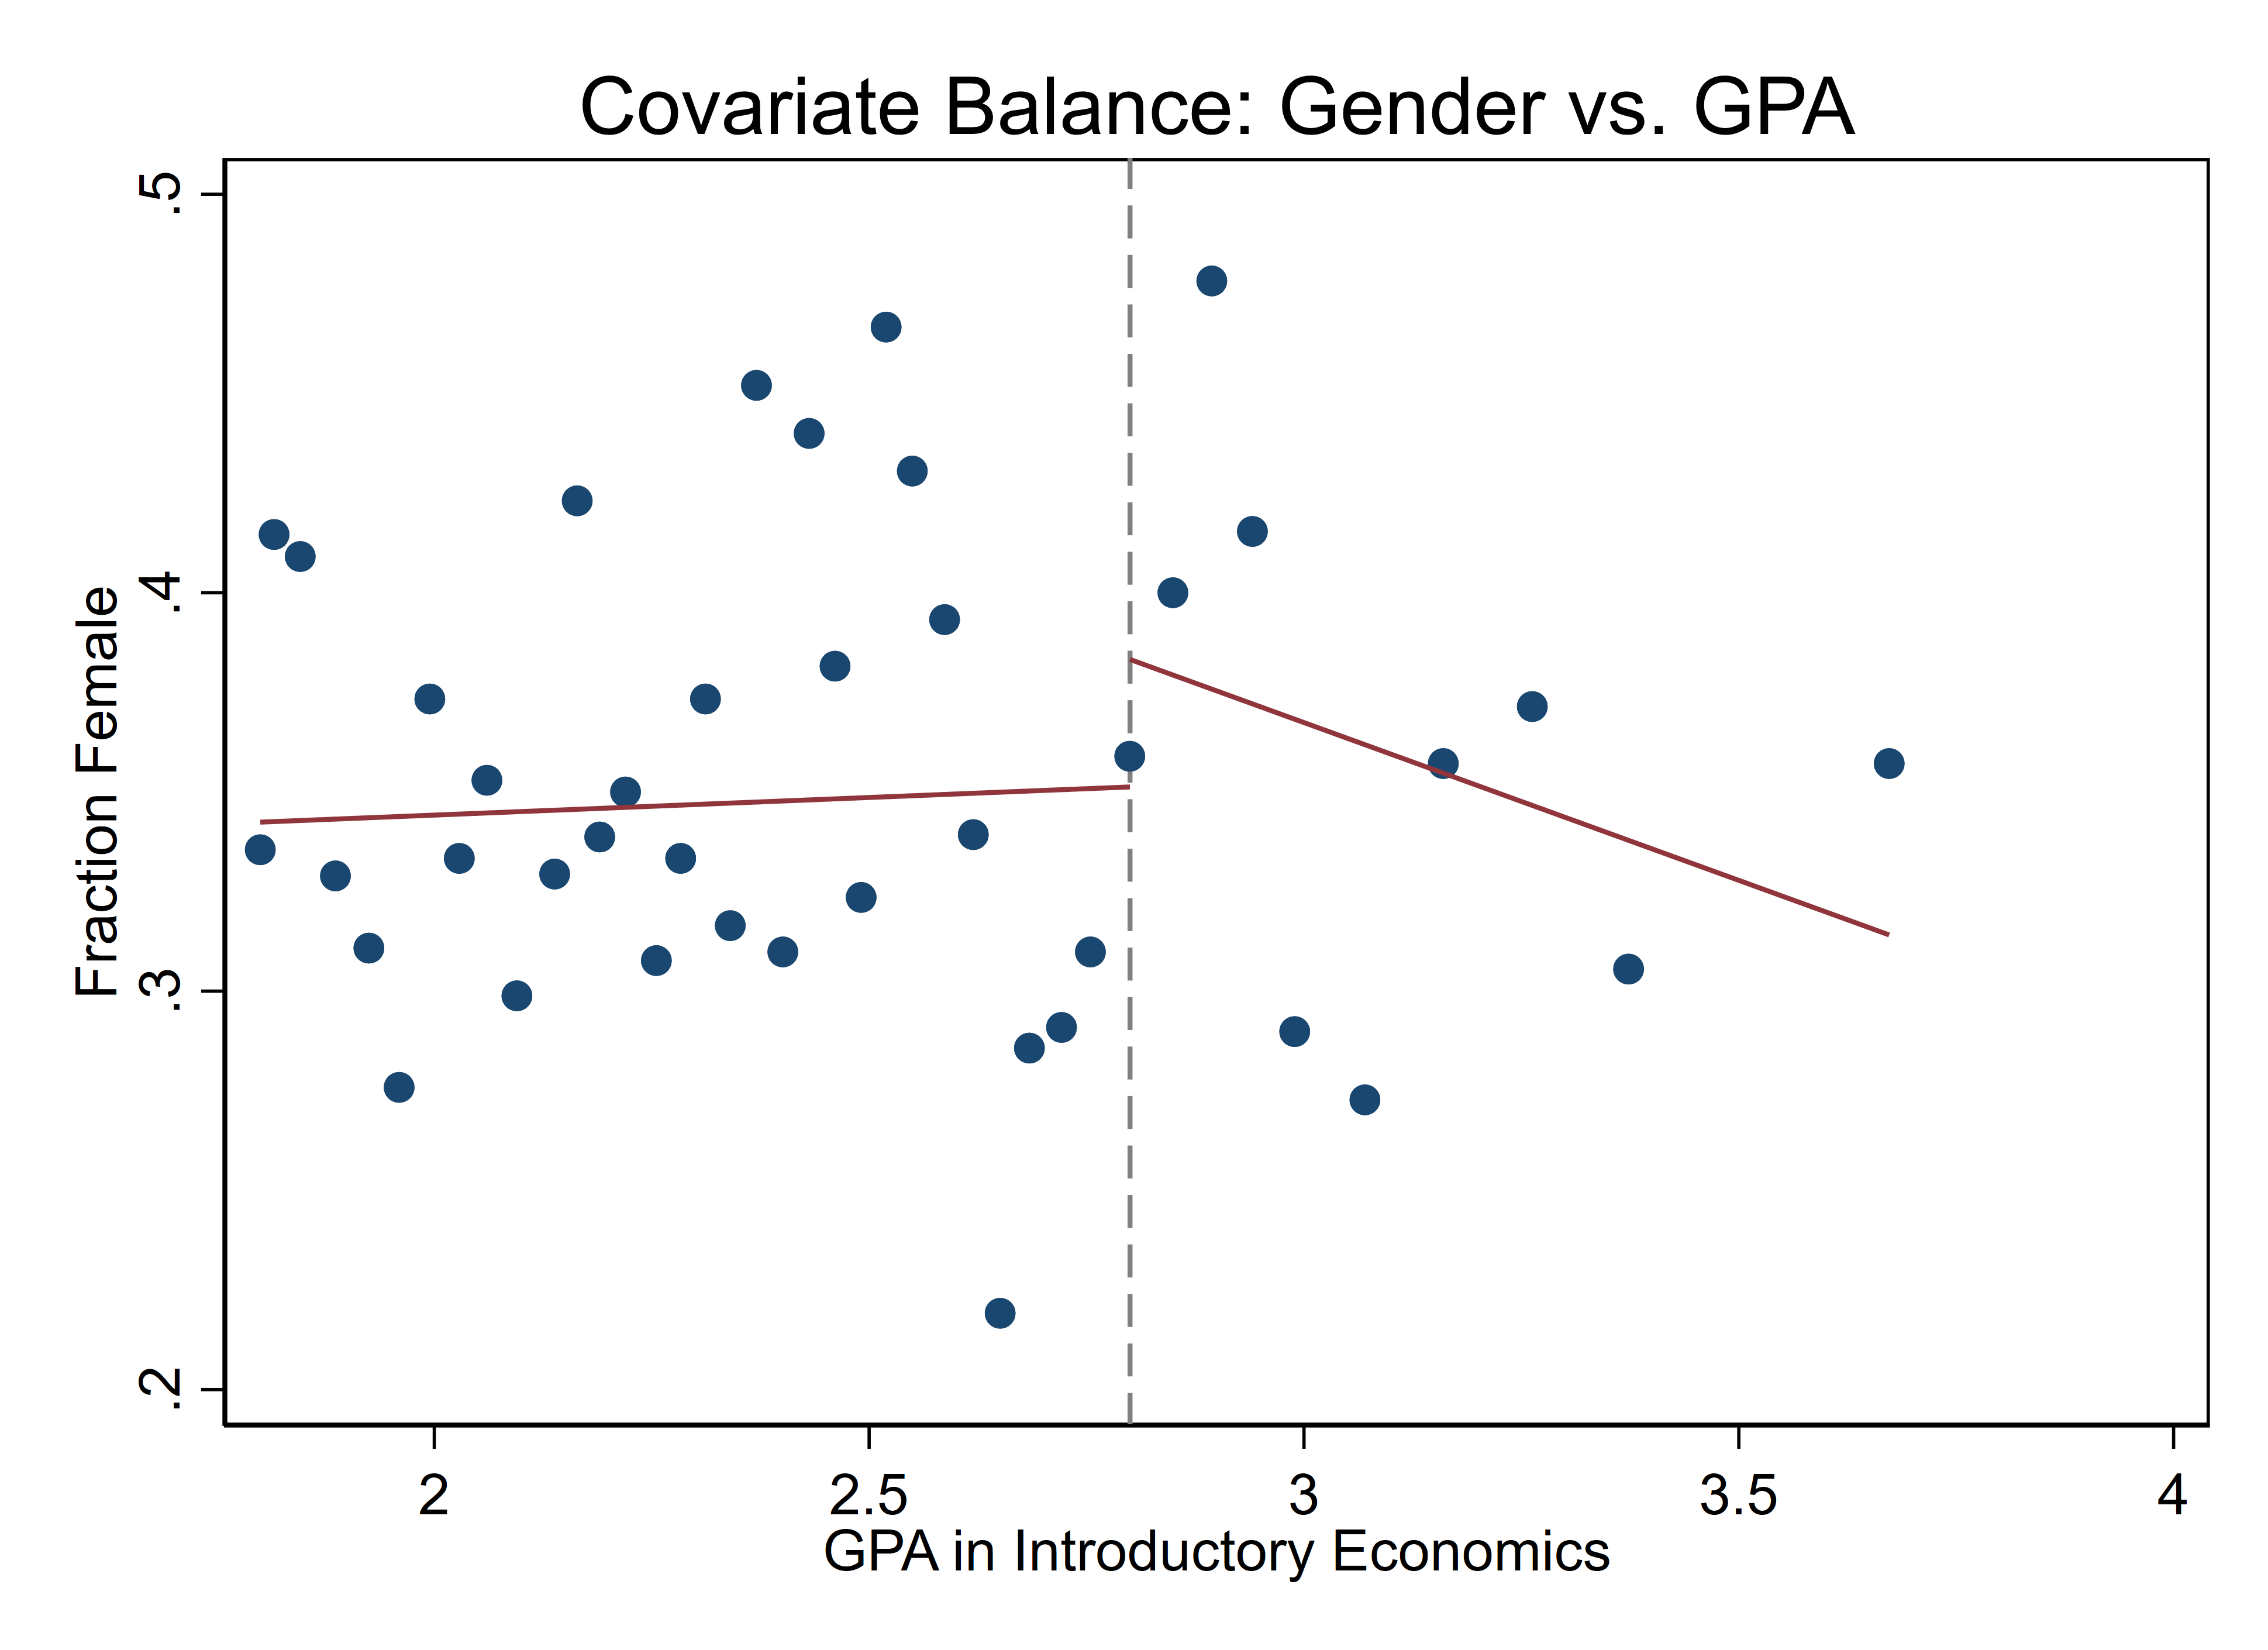
\includegraphics[width=0.9\textwidth]{figure/econ_female.png}

\end{frame}


%------------------------------------------------------------
% STEP 2: Sorting Test
%------------------------------------------------------------

\begin{frame}{Step 2: Test Sorting Behavior}
	\begin{itemize}
		\item Plot the \textbf{distribution (density) of the running variable} (GPA)
		around the cutoff
		\vspace{0.2cm}
		\item If students can \textbf{manipulate} their GPA to just exceed 2.8
		(e.g.\ by disputing grades or retaking the course), we would see:
		\begin{itemize}
			\vspace{0.2cm}
			\item A spike in the density \emph{just above} GPA = 2.8
			\vspace{0.2cm}
			\item A dip in the density \emph{just below} GPA = 2.8
		\end{itemize}
		\vspace{0.2cm}
		\item $H_0$: no density discontinuity at the cutoff
		\vspace{0.2cm}
		\item Non-rejection (p-value $> 0.05$) supports the validity of the RDD
	\end{itemize}
\end{frame}


\begin{frame}[fragile]{STATA Command: rddensity}{Sorting Test}
	\begin{itemize}
		\item Syntax:
\begin{lstlisting}
rddensity runvar [if] [in] [, options]
\end{lstlisting}

		\item Example:
\begin{lstlisting}
rddensity gpa_econ, c(2.8) all plot
graph export figure/econ_density.png, replace
\end{lstlisting}

		\vspace{0.2cm}
		\item \textbf{gpa\_econ}: the running variable whose density we test
		\vspace{0.2cm}
		\item \textbf{c(2.8)}: the cutoff value
		\vspace{0.2cm}
		\item \textbf{plot}: display the estimated density on both sides
	\end{itemize}
\end{frame}


\begin{frame}{Test Sorting Behavior}{}

	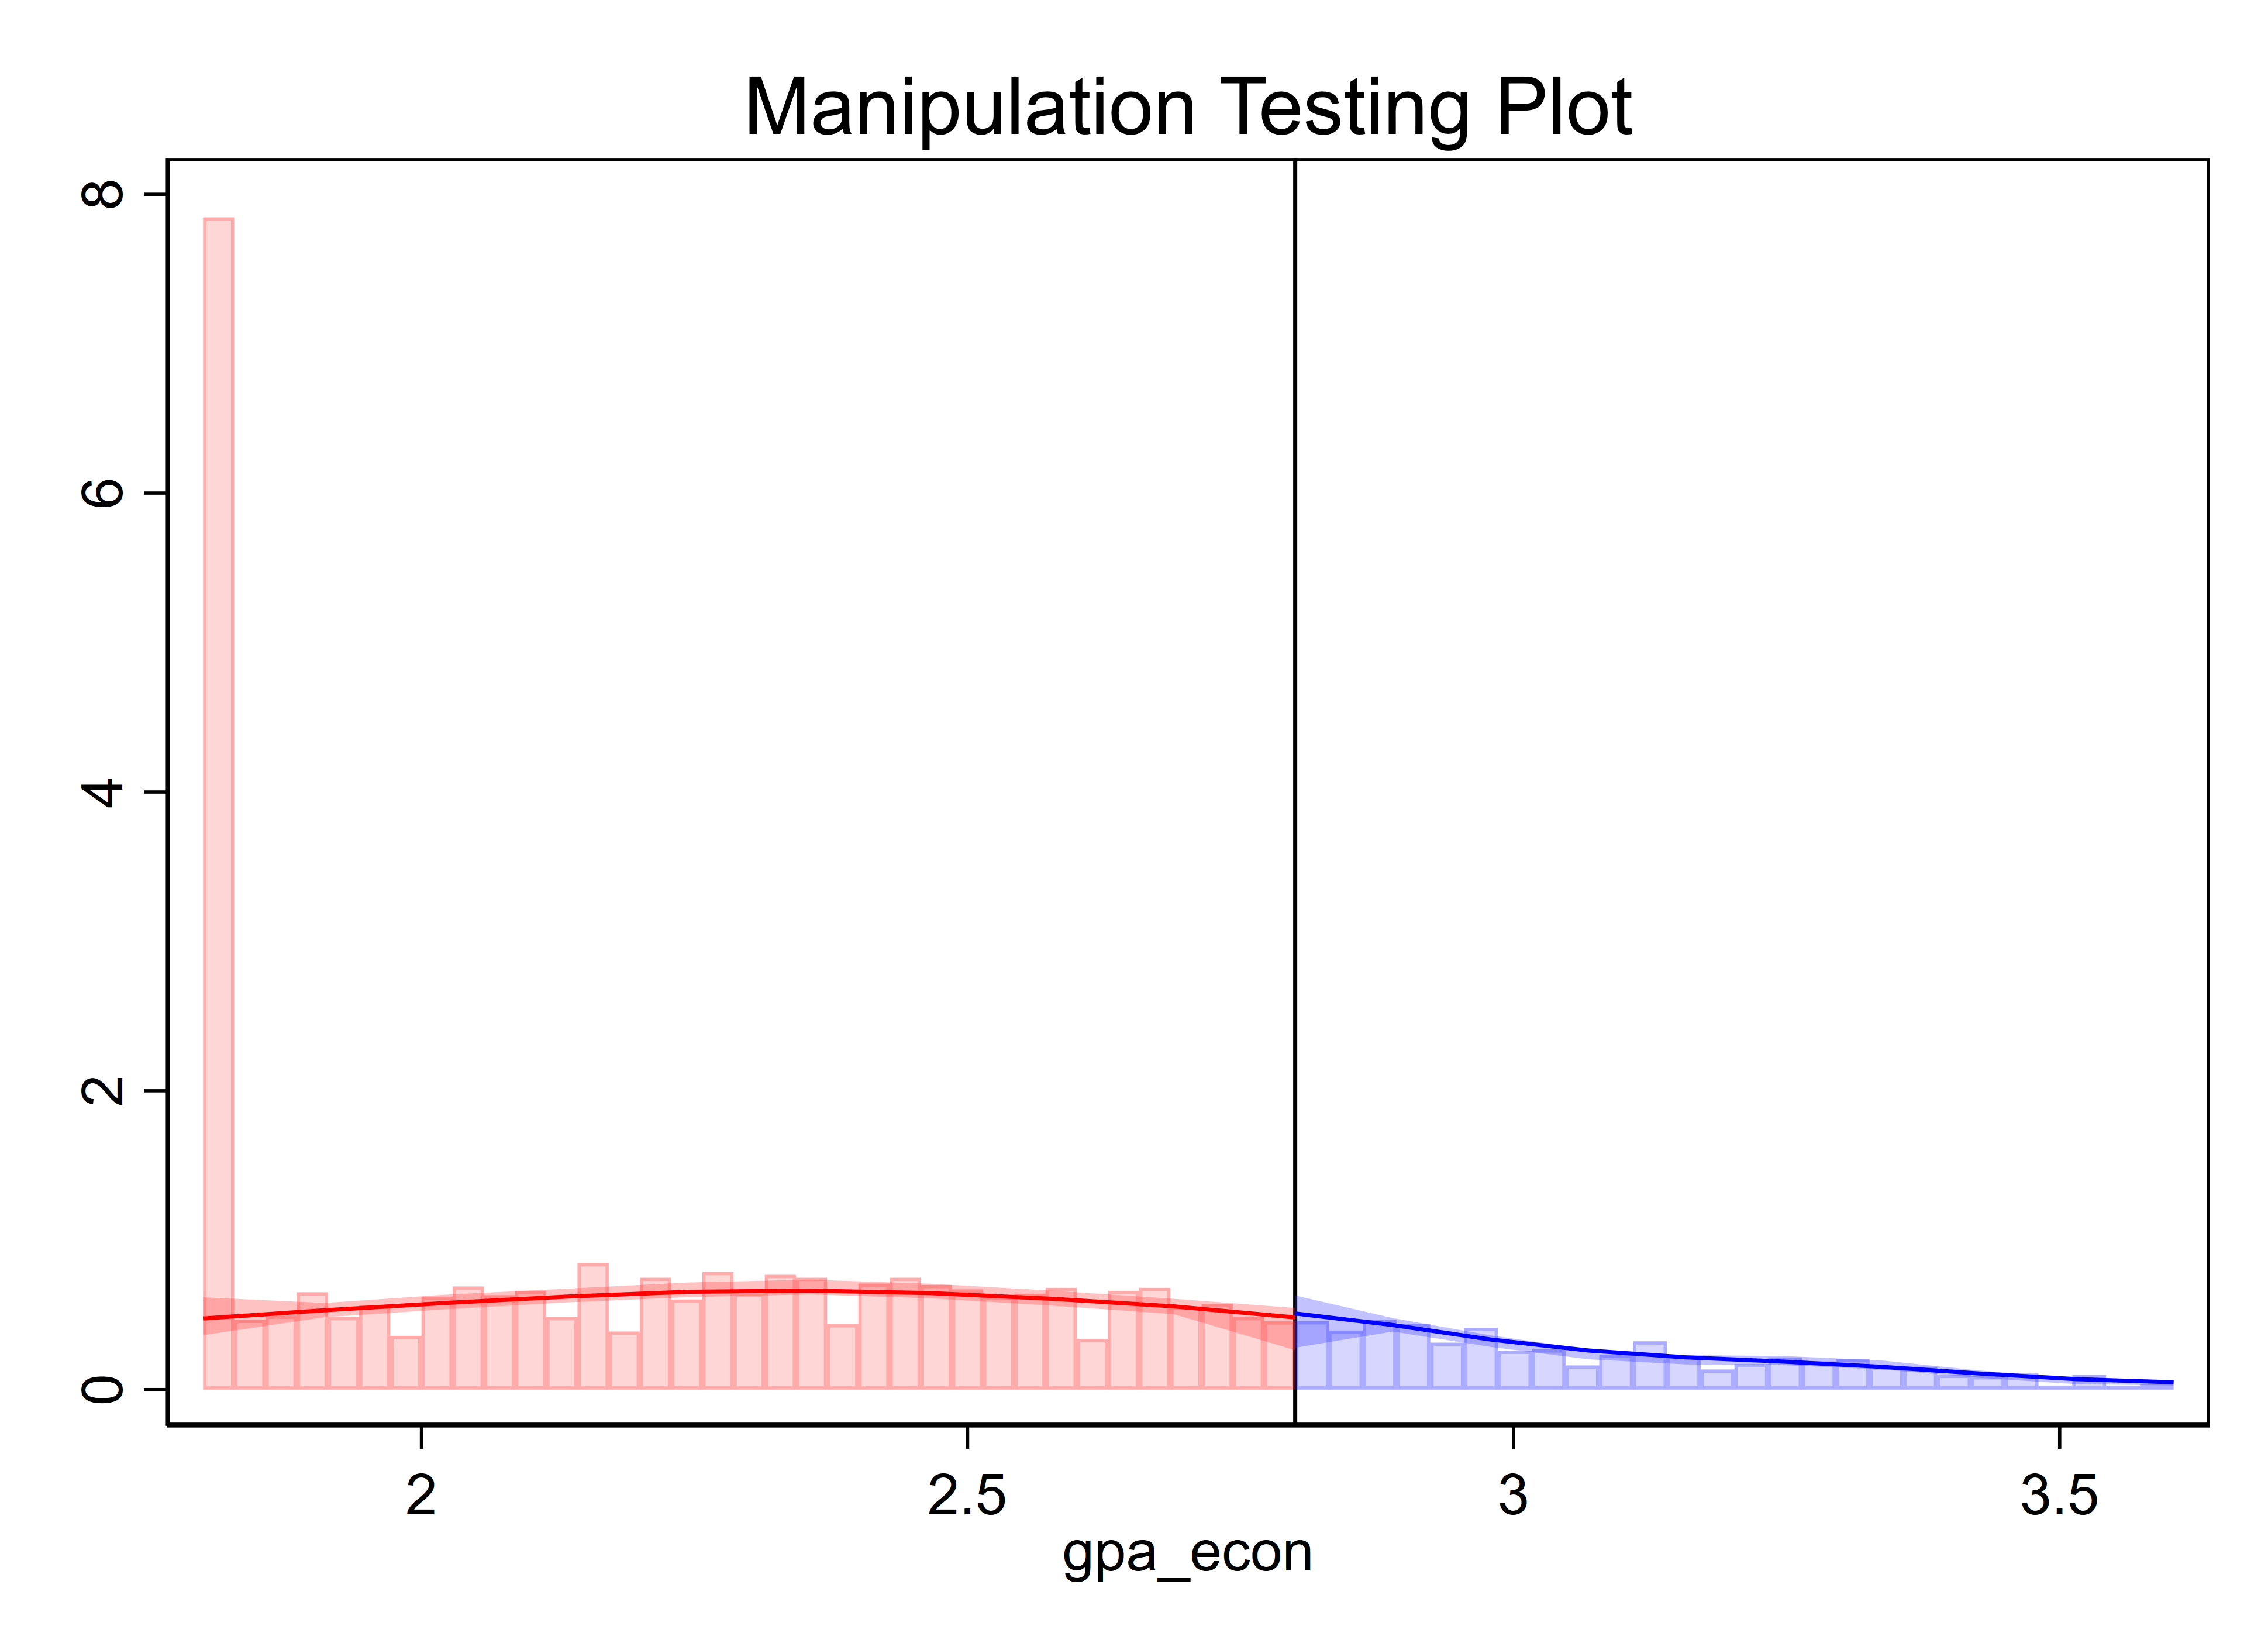
\includegraphics[width=0.9\textwidth]{figure/econ_density.png}

\end{frame}


%------------------------------------------------------------
% STEP 3: Preparation for Estimation
%------------------------------------------------------------

\begin{frame}[fragile]{Step 3: Preparation for Estimation}
	\begin{itemize}
		\item Generate centered running variable $A_i - c$ and polynomial terms
		\item Generate interaction terms between $Z_i$ and $(A_i - c)$
\begin{lstlisting}
* Center running variable at cutoff
gen gpa_c  = gpa_econ - 2.8
gen gpa_c2 = gpa_c^2

* Interaction terms (allow different slopes on each side)
gen above_gpa_c  = above * gpa_c
gen above_gpa_c2 = above * gpa_c2
\end{lstlisting}
		\vspace{0.2cm}
		\item \textbf{above}: $Z_i = \mathbf{1}[A_i \geq 2.8]$ (already in dataset)
		\vspace{0.2cm}
		\item \textbf{gpa\_c}: centered running variable (= 0 at the cutoff)
		\vspace{0.2cm}
		\item \textbf{above\_gpa\_c}: allows the slope to differ on each side
	\end{itemize}
\end{frame}


%------------------------------------------------------------
% STEP 4: Estimation
%------------------------------------------------------------

\begin{frame}[fragile]{Step 4: Estimation}{First Stage and Reduced Form}
	\begin{itemize}
		\item \textbf{First stage}: effect of crossing GPA 2.8 on economics enrollment
		\item \textbf{Reduced form}: effect of crossing GPA 2.8 on log wages (ITT)
\begin{lstlisting}
* First stage: Z_i -> D_i
reg econ_major above gpa_c above_gpa_c, cl(gpa_c)

* Reduced form: Z_i -> Y_i  (Intent-to-Treat)
reg logwage_1718 above gpa_c above_gpa_c if employed_1718, cl(gpa_c)

* Manual Wald/LATE = reduced form coeff / first stage coeff
\end{lstlisting}
		\vspace{0.2cm}
		\item \textbf{cl(gpa\_c)}: cluster standard errors at the GPA level
		\vspace{0.2cm}
		\item \textbf{above coefficient}: the RDD estimate on each regression
	\end{itemize}
\end{frame}


\begin{frame}[fragile]{Step 4: Estimation}{Fuzzy RDD -- 2SLS (LATE)}
	\begin{itemize}
		\item \textbf{Fuzzy IV (2SLS)}: instrument $D_i$ (\texttt{econ\_major}) with $Z_i$ (\texttt{above})
		\item The IV estimate $= $ LATE: causal effect for compliers
\begin{lstlisting}
* Fuzzy RDD: 2SLS
ivregress 2sls logwage_1718 gpa_c above_gpa_c
    (econ_major = above) if employed_1718, vce(cl gpa_c)

* OLS (biased upward due to ability selection -- shown for comparison)
reg logwage_1718 econ_major gpa_c above_gpa_c
    if employed_1718, cl(gpa_c)
\end{lstlisting}
		\vspace{0.2cm}
		\item Syntax \texttt{(econ\_major = above)}: instrument \texttt{econ\_major} with \texttt{above}
		\vspace{0.2cm}
		\item OLS $> $ LATE: unobserved ability biases OLS upward
	\end{itemize}
\end{frame}


\begin{frame}[fragile]{Step 4: Estimation}{Nonparametric -- rdrobust}
	\begin{itemize}
		\item Use \texttt{rdrobust} with \texttt{fuzzy()} for data-driven bandwidth selection
\begin{lstlisting}
* First stage (sharp RDD on treatment)
rdrobust econ_major gpa_econ, c(2.8) kernel(tri) all

* Reduced form
rdrobust logwage_1718 gpa_econ if employed_1718,
    c(2.8) kernel(tri) all

* Fuzzy RDD: LATE
* fuzzy() specifies the actual treatment D_i
rdrobust logwage_1718 gpa_econ if employed_1718,
    c(2.8) fuzzy(econ_major) kernel(tri) all

* Covariate balance tests
foreach var in sat_score female urm zip_income {
    rdrobust `var' gpa_econ, c(2.8) kernel(tri)
}
\end{lstlisting}
	\end{itemize}
\end{frame}


%------------------------------------------------------------
% STEP 5: Robustness Checks
%------------------------------------------------------------

\begin{frame}[fragile]{Step 5: Robustness Checks}
	\begin{itemize}
		\item Try different \textbf{bandwidth values}
\begin{lstlisting}
foreach h in 0.3 0.4 0.5 0.6 0.8 1.0 {
    rdrobust logwage_1718 gpa_econ if employed_1718,
        c(2.8) h(`h') fuzzy(econ_major) kernel(tri)
    display "h=`h': LATE=" e(tau_cl)
}
\end{lstlisting}
		\vspace{0.1cm}
		\item Try \textbf{quadratic polynomial} in the running variable
\begin{lstlisting}
ivregress 2sls logwage_1718 gpa_c gpa_c2 above_gpa_c above_gpa_c2
    (econ_major = above) if employed_1718, vce(cl gpa_c)
\end{lstlisting}
		\vspace{0.1cm}
		\item Check \textbf{additional outcomes}
\begin{lstlisting}
rdrobust employed_1718 gpa_econ, c(2.8) fuzzy(econ_major) kernel(tri)
rdrobust grad_school   gpa_econ, c(2.8) fuzzy(econ_major) kernel(tri)
\end{lstlisting}
	\end{itemize}
\end{frame}


% ================================================================
% R Example: Bleemer & Mehta (2022) -- Fuzzy RDD
% ================================================================

\title[]
{R Example: Fuzzy RDD}

\author
{}

\institute{}

\date
{}

\begin{frame}{}
	\titlepage
\end{frame}


\begin{frame}{Bleemer \& Mehta (2022)}{R Implementation}
	\begin{itemize}
		\item Install and load required R packages:
		\begin{itemize}
			\vspace{0.2cm}
			\item \texttt{haven} (read Stata .dta files)
			\vspace{0.2cm}
			\item \texttt{rdrobust} (rdrobust, rdplot, rdbwselect)
			\vspace{0.2cm}
			\item \texttt{rddensity} (density test and plot)
			\vspace{0.2cm}
			\item \texttt{AER} (ivreg -- 2SLS estimation)
		\end{itemize}
		\vspace{0.2cm}
		\item Use \texttt{simulated\_econ\_rdd.dta}
		\vspace{0.2cm}
		\item See \texttt{exercise\_r\_econ\_rdd.R}
	\end{itemize}
\end{frame}


\begin{frame}[fragile]{Package Installation and Data Loading}
\begin{lstlisting}[language=R]
# Install once
install.packages(c("haven", "rdrobust", "rddensity", "AER", "dplyr"))

library(haven);    library(rdrobust)
library(rddensity); library(AER);  library(dplyr)

# Load simulated data
data   <- read_dta("simulated_econ_rdd.dta")
cutoff <- 2.8
summary(data)

# Subsample: employed workers (for wage regressions)
data_emp <- data |> filter(employed_1718 == 1, !is.na(logwage_1718))
\end{lstlisting}
\end{frame}


\begin{frame}[fragile]{Step 1: Graphical Analysis}{First Stage and Reduced Form}
\begin{lstlisting}[language=R]
# First stage: P(Economics Major) by GPA
rdplot(y = data$econ_major, x = data$gpa_econ, c = cutoff,
       title   = "First Stage: GPA Cutoff and Economics Enrollment",
       x.label = "GPA in Introductory Economics",
       y.label = "P(Economics Major)")

# Reduced form: Log wages by GPA
rdplot(y = data_emp$logwage_1718, x = data_emp$gpa_econ, c = cutoff,
       title   = "Reduced Form: GPA Cutoff and Log Wages",
       x.label = "GPA in Introductory Economics",
       y.label = "Log Wages (2017-2018)")

# Covariate balance: SAT score (should show no jump)
rdplot(y = data$sat_score, x = data$gpa_econ, c = cutoff,
       title   = "Covariate Balance: SAT Score",
       x.label = "GPA in Introductory Economics",
       y.label = "SAT Score")
\end{lstlisting}
\end{frame}


\begin{frame}[fragile]{Step 2: Testing for Sorting Behavior}
\begin{lstlisting}[language=R]
# rddensity: Cattaneo, Jansson, Ma (2020)
# H0: no density discontinuity at GPA = 2.8
dens_test <- rddensity(X = data$gpa_econ, c = cutoff)
summary(dens_test)
# p-value > 0.05: no evidence of manipulation -> RDD valid

# Visual: density plot around cutoff
rdplotdensity(dens_test, data$gpa_econ,
              title = "McCrary Test: GPA Density at Cutoff")
\end{lstlisting}
\end{frame}


\begin{frame}[fragile]{Step 3: Data Preparation for Estimation}
\begin{lstlisting}[language=R]
# Center running variable and create interaction terms
data <- data |>
  mutate(gpa_c        = gpa_econ - cutoff,
         gpa_c2       = gpa_c^2,
         above_gpa_c  = above * gpa_c,
         above_gpa_c2 = above * gpa_c^2)

data_emp <- data |> filter(employed_1718 == 1, !is.na(logwage_1718))
\end{lstlisting}
\end{frame}


\begin{frame}[fragile]{Step 4: Estimation}{First Stage and Reduced Form}
\begin{lstlisting}[language=R]
# First stage: Z_i -> D_i
fs <- lm(econ_major ~ above + gpa_c + above_gpa_c, data = data)
cat("First stage jump:", round(coef(fs)["above"], 4), "\n")

# Reduced form: Z_i -> Y_i  (Intent-to-Treat)
rf <- lm(logwage_1718 ~ above + gpa_c + above_gpa_c, data = data_emp)
cat("Reduced form:", round(coef(rf)["above"], 4), "\n")

# Manual LATE = Reduced Form / First Stage
cat("LATE (manual):", round(coef(rf)["above"]/coef(fs)["above"], 4), "\n")
\end{lstlisting}
\end{frame}


\begin{frame}[fragile]{Step 4: Estimation}{Fuzzy RDD -- 2SLS (LATE)}
\begin{lstlisting}[language=R]
# Fuzzy RDD (2SLS): instrument econ_major with above
fuzzy_iv <- ivreg(
  logwage_1718 ~ econ_major + gpa_c + above_gpa_c |
                 above      + gpa_c + above_gpa_c,
  data = data_emp)
cat("LATE (2SLS):", round(coef(fuzzy_iv)["econ_major"], 4), "\n")

# OLS (biased upward -- for comparison)
ols <- lm(logwage_1718 ~ econ_major + gpa_c + above_gpa_c,
          data = data_emp)
cat("OLS (biased):", round(coef(ols)["econ_major"], 4), "\n")
# OLS > LATE: unobserved ability biases OLS upward
\end{lstlisting}
\end{frame}


\begin{frame}[fragile]{Step 4: Estimation}{Nonparametric -- rdrobust}
\begin{lstlisting}[language=R]
# First stage
summary(rdrobust(data$econ_major, data$gpa_econ,
                 c = cutoff, kernel = "tri", all = TRUE))

# Reduced form
summary(rdrobust(data_emp$logwage_1718, data_emp$gpa_econ,
                 c = cutoff, kernel = "tri", all = TRUE))

# Fuzzy RDD: LATE (fuzzy= specifies D_i; rdrobust uses Z_i as instrument)
rdd_fuzzy <- rdrobust(y     = data_emp$logwage_1718,
                      x     = data_emp$gpa_econ,
                      fuzzy = data_emp$econ_major,
                      c = cutoff, kernel = "tri", all = TRUE)
summary(rdd_fuzzy)

# Covariate balance
for (v in c("sat_score", "female", "urm", "zip_income")) {
  b <- rdrobust(data[[v]], data$gpa_econ, c = cutoff, kernel = "tri")
  cat(v, ": p =", round(b$pv[1], 4), "\n")
}
\end{lstlisting}
\end{frame}


\begin{frame}[fragile]{Step 5: Robustness Checks}
\begin{lstlisting}[language=R]
# Bandwidth sensitivity
for (h in c(0.3, 0.4, 0.5, 0.6, 0.8, 1.0)) {
  rdd_h <- rdrobust(y = data_emp$logwage_1718, x = data_emp$gpa_econ,
                    fuzzy = data_emp$econ_major,
                    c = cutoff, h = h, kernel = "tri")
  cat(sprintf("h=%.1f: LATE = %.4f (SE = %.4f)\n",
              h, rdd_h$coef[1], rdd_h$se[3]))
}

# Quadratic polynomial
fuzzy_quad <- ivreg(
  logwage_1718 ~ econ_major + gpa_c + gpa_c2 + above_gpa_c + above_gpa_c2 |
                 above      + gpa_c + gpa_c2 + above_gpa_c + above_gpa_c2,
  data = data_emp)
cat("Quadratic LATE:", round(coef(fuzzy_quad)["econ_major"], 4), "\n")
\end{lstlisting}
\end{frame}



\end{document} 
